\documentclass[12pt, 
openright, 
oneside, 
%twoside, %TCC: Se seu texto tem mais de 100 páginas, descomente esta linha e comente a anterior
a4paper,    
%english,   
brazil]{facom-ufu-abntex2}



\autor{Igor Batista Fernandes} 
\data{2018}
\orientador{Profa. Maria Adriana Vidigal de Lima} 
\titulo{Desenvolvimento de uma game engine 2D multiplataforma utilizando
OpenGL e Java } 

\begin{document}
\pagenumbering{arabic}

\pagestyle{plain}


% ----------------------------------------------------------
% ELEMENTOS PRÉ-TEXTUAIS

\imprimircapa

\begin{folhadeaprovacao}

  \begin{center}
    {\ABNTEXchapterfont\large\imprimirautor}

    \vspace*{\fill}\vspace*{\fill}
    {\ABNTEXchapterfont\bfseries\Large\imprimirtitulo}
    \vspace*{\fill}
    
    \hspace{.45\textwidth}
    \begin{minipage}{.5\textwidth}
    \imprimirpreambulo
    \end{minipage}%
    \vspace*{\fill}
   \end{center}
    
   %Trabalho aprovado. 
   \imprimirlocal, XX de XX de 2018: %TCC:

   \assinatura{\textbf{\imprimirorientador} \\ Orientador}  
   \assinatura{\textbf{Professor}}% \\ Convidado 1} %TCC:
   \assinatura{\textbf{Professor}}% \\ Convidado 2} %TCC:
   %\assinatura{\textbf{Professor} \\ Convidado 3}
   %\assinatura{\textbf{Professor} \\ Convidado 4}
      
   \begin{center}
    \vspace*{0.5cm}
    {\large\imprimirlocal}
    \par
    {\large\imprimirdata}
    \vspace*{1cm}
  \end{center}
  
\end{folhadeaprovacao}
%-------------------------------------------
% RESUMO

//TODO : tirar game design document do resumo e do 
abstract
//TODO : capítulo de trabalhos correlatos pode ser colocado como seção no capítulo da arquitetura NARVAL ao final (como arquiteturas correlatas)


\begin{resumo} 

Este trabalho propõe a criação de uma Game Engine multiplataforma para desktop intitulada Narval e a subsequente elaboração de um protótipo de jogo.
A implementação de código será realizada na linguagem Java e através da API gráfica OpenGL usando GLFW (OpenGL Frame Work). 
A elicitação dos requisitos do jogo será documentada em um artefato denominado \textit{Game Design Document} que permite estruturar, sistematizar e organizar 
o processo de construção.
O jogo será elaborado utilizando técnicas de algoritmos procedurais para geração de artes e ambientes, inteligência artificial para o comportamento de Non Playable Characters (NPC) e padrões de projeto aplicados em jogos.
 
 \vspace{\onelineskip}
 \noindent
 \textbf{Palavras-chave}: Indie Game, Game Design Document, Jogos, Java, OpenGL, Game Engine, Artificial Intelligence
\end{resumo}

\begin{abstract} 
This work proposes to develop a multiplataform game engine for desktop entitled Narval and a subsequent game prototype elaboration. 
The code implementation will be done in Java through the API OpenGL using GLFW (OpenGL Frame Work).
The elicitation of requisites for the game will be documented in an artifact called Game Design Document which allows to structure, systematize and organize the process of building a game.
The game will be elaboreted using techniques of procedural algorithms to generate art and environment, artificial intelligence for Non Playable Characters (NPC) behaviours and design patterns applied to games.

 \vspace{\onelineskip}
    
 \noindent
 \textbf{Keywords}: Indie Game, Game Design Document, Jogos, Java, OpenGL, Game Engine, Artificial Intelligence %TCC:
\end{abstract}
\cleardoublepage

\begin{figure}[H]
	\centering
	
\includegraphics[width=\textwidth]{imagens/logo.png}
\end{figure}
\clearpage


% ------------------------------------------
% LISTA DE FIGURAS

\pdfbookmark[0]{\listfigurename}{lof}
\listoffigures*
\cleardoublepage

% ------------------------------------------
% LISTA DE TABELAS

\pdfbookmark[0]{\listtablename}{lot}
\listoftables*
\cleardoublepage

% ------------------------------------------
% LISTA DE CÓDIGOS
\pdfbookmark[0]{\listtablename}{lol}
\lstlistoflistings
\cleardoublepage

% ------------------------------------------
% LISTA DE ABREVIATURAS OU SIGLAS



\begin{siglas} 
  \item[GDD] Game Design Document 
  \item[API] Application Programming Interface
  \item[MVC] Model-view-controller
  \item[OpenGL] Open Graphics Library
  \item[GPU] Graphics Processing Unit
  \item[GLFW] Graphics Library Framework
  \item[GLSL] OpenGL Shading Language
  \item[NPC] Non Playable Character
  \item[HUD] Heads-Up Display
  \item[FPS] Frames per second
  \item[px] Pixel (Unidade de medida)
  \item[VBO] Vertex Buffer Object
  \item[VAO] Vertex Array Object
  \item[AABB] Axis Aligned Bouding Box
  \item[NDC] Normalized Device Coordinates
  \item[GLM] OpenGL Mathematics Library
  \item[IA] Inteligência Artificial
  \item[PCM] Pulse-code modulation 
  \item[FOV] Field Of View
\end{siglas}


% SUMÁRIO
% ---
\pdfbookmark[0]{\contentsname}{toc}
\tableofcontents*
\cleardoublepage


% ------------------------------------------
% COMEÇAR O TEXTO

%\textual

% ------------------------------------------% INTRODUÇÃO

% colocar como subitem 
%\chapter*[Introdução]{Introdução}
%\addcontentsline{toc}{chapter}{Introdução}

\chapter{Introdução}

\section{Visão Geral da Proposta}
Estima-se que o mercado internacional de jogos movimentará aproximadamente 108.9
bilhões de dólares distribuídos entre 2.2 bilhões de jogadores em 2017. Destes, 58\%
representam os segmentos de PC e consoles \cite{GameMarketArticle}. Além de ser uma área
comercial lucrativa é também interdisciplinar e aproxima
diversos conceitos de Computação, Design gráfico, Música, Artes e outras esferas do
conhecimento.
Para a elaboração de um projeto bem construído e com alto potencial de
sucesso é necessário respeitar as etapas de pré-produção, produção, testes
e pós-produção. Ao longo de todas as etapas serão definidas estratégias de
implementação em linguagens orientadas a objetos, engenharia de software, padrões de projeto
voltados para jogos e metodologias ágeis.

%Objetivo
\section{Objetivo}
Este projeto propõe portanto a construção de uma game engine, também traduzida como motor de jogo. Para isso será utilizado a linguagem Java e a biblioteca LWJGL, que incorpora a biblioteca OpenGL, GLFW e outras necessárias ao projeto.
Desenvolvida pela Khronos Group a API OpenGL fornece uma ampla gama de soluções para aplicações gráficas, sendo acelerada diretamente em
hardware, multiplataforma e robusta. Esses fatores culminaram na sua escolha como o componente responsável pela renderização da engine. Para a parte de áudio será utilizada a biblioteca OpenAL e para o modulo de física a biblioteca jBox2D. 
Ao fim de seu desenvolvimento será ainda construído um protótipo de jogo para demonstrar as funcionalidades da mesma. %Esse protótipo será construído utilizando o Game Design Document (GDD), definido em seu próprio capítulo.

\section{Justificativa e Motivação}
O consumo cada vez maior deste tipo de produto pelo público de todas as idades traz cada vez mais oportunidades de trabalho e aprendizagem.
A insuficiência de materiais em língua portuguesa sobre os processos de desenvolvimento e planejamento de jogos é um grande instigador desse trabalho. Neste contexto, esse trabalho aborda todas as etapas pelas quais uma engine passa para torna-se um software que será distribuído e utilizado por pessoas do mundo todo.
Embora haja diversas opções de Engines no mercado como Unity, Unreal, CryEngine e afins, a grande maioria é de código fechado, o que torna extremamente dificil senão impossível de modificá-la para as necessidades especias de um projeto. Além deste fato, para comercializar os produtos produzidos nelas é necessário pagar uma porcentagem da revenda obtida com o produto lançado. Portanto, para este projeto será desenvolvida uma Engine própria, para ter-se uma maior flexibilidade de implementação e para ter uma licença de software próprio.

\section{Organização do Trabalho}
//TODO: editar seção
No Capítulo \ref{cap:Metodologia} está descrita a Metodologia utilizada neste trabalho. As bases teóricas: Manutenção de Sistema, Banco de Dados, Falta de Informações, Projeto de Banco de Dados e Refatoração em Banco de Dados são encontradas no Capítulo \ref{cap:ReferencialTeorico}. No Capítulo \ref{cap:BancoSIAF} é apresentado o Banco de Dados do SIAF. O Desenvolvimento do trabalho de remodelagem de dados compõe o Capítulo \ref{cap:Desenvolvimento}. Finalmente, o Capítulo \ref{cap:Conclusao} expõe as Conclusões obtidas do trabalho desenvolvido e apresenta perspectivas para Trabalhos Futuros.


\iffalse
\section{Metodologia}


Este trabalho se classifica como uma pesquisa aplicada, sendo o método de desenvolvimento baseado nas etapas a seguir:

Etapa 1 – Revisão sistemática em desenvolvimento de jogos
\begin{itemize}
\item Desenvolvimento de Jogos estilo RPG - levantamento bibliográfico, identificação e organização dos trabalhos relacionados e do estado da arte;
\item Pesquisa documental sobre engenharia de software e padrões de projeto aplicada a jogos;
\item Pesquisa documental sobre o uso de metodologias ágeis no desenvolvimento de jogos.
\end{itemize}

Etapa 2 – Projeto do jogo identificando os conceitos a serem aplicados 
\begin{enumerate}
\item Pré-Projeto: análise de mercado, tendências e viabilidade;
definição da ideia do seu jogo; atividades a serem realizadas;
equipe.
\item Pré-Produção: elaboração do Game Design Document, elaboração do Roteiro, elaboração do Documento de Arte e Design Gráfico; criação de protótipos para testar ideias, mecânicas e conceitos;
\item Plano de Produção: criação de um cronograma e planejamento dos ciclos de trabalho da produção, considerando o desenvolvimento do jogo utilizando uma  metodologia ágil (SCRUM). Desenvolvimento de uma game engine/framework para a construção do jogo. Análise de requisitos do jogo. Os requisitos serão documentados usando diagramas de casos de uso em paralelo ao uso do GDD.
\end{enumerate}

Etapa 3 – Implementação do jogo em formato digital. O desenvolvimento será dividido nos seguintes ciclos:
\begin{enumerate}
\item Desenvolvimento e testes de unidade do módulo gráfico
(cenários, animações, mecânica).
\item Desenvolvimento e testes de unidade do módulo de físicas
(colisões em geral).
\item Desenvolvimento e teste de unidade do módulo de áudio.
\item Desenvolvimento de interfaces e ferramentas.
\item Desenvolvimento das artes e teste de fluxo.
\item Teste de sistema e ajustes.
\end{enumerate}
Etapa 4 – Testes e avaliação do jogo.
\begin{enumerate}
\item Etapa alfa. Consiste de um período de testes com um grupo seleto de pessoas.
\item Etapa Beta. Etapa de testes aberta e já próxima do lançamento final.
\item Lançamento.
\end{enumerate}
\fi


% ------------------------------------------
% REFERENCIAL TEÓRICO

\chapter{Revisão Bibliográfica}


\label{sec:refteo}
\section{Computação gráfica}
Computação gráfica refere-se a tudo que envolve criação ou manipulação de imagens no computador, incluindo animações \cite{ComputerGraphicsIntro}. Este ramo possui aplicações em diversas áreas, tais como: Jogos, Arquitetura, Cinema, Medicina, Artes e várias outras. Toda a computação gráfica atual é baseada em cálculos matemáticos para sintetizar pixels em uma tela 2D. Esse processo se dá através de um pipeline por onde primitivas gráficas são manipuladas para obter o resultado final mostrado na tela do usuário.
\section{OpenGL}
A API (Application Programming Interface) OpenGL fornece um conjunto de funções para manipulações gráficas \cite{LearnOpenGL}, sendo acelerada diretamente em hardware, multiplataforma e robusta. Embora comumente referida como uma API, o OpenGL é, por si só, um conjunto de especificações que determinam o resultado/saída de cada função e como devem ser executadas. Fica a cargo dos manufaturadores de placas gráficas implementarem a operação da função, respeitando as especificações do documento desenvolvido e mantido pela Khronos Group \cite{KhronosOpenGLSpecification}.

 O OpenGL foi lançado em 1992 como uma resposta direta a necessidade de se padronizar o conjunto de instruções usado em hardwares com interface gráfica. Até setembro de 2006 o padrão foi mantido pela ARB (Architecture Review Board), um conselho formado por empresas de grande renome no ramo como HP, IBM, Intel, NVIDIA, Dell e a própria fundadora, a Silicon Graphics. Em setembro de 2006 o conselho ARB tornou-se o OpenGL Working Group gerido e mantido pelo consórcio Khronos Group para Open Standard APIs\cite{OpenGLAbout}.
 
\section{Game Engine}
Define-se como game engine um sistema composto de outros sub sistemas cujo trabalho em coesão provêm todas as funcionalidades necessárias para o desenvolvimento de um jogo. Uma arquitetura direcionada a dados é o que diferencia uma game engine de um pedaço de software que é o jogo, mas não uma engine \cite{GameEngineArchitecture}. 

Portanto, game engine é um software extensível e pode ser usado como fundação para diferentes tipos e gêneros de jogos sem mudanças maiores no seu núcleo. Embora uma game engine ideal deva ser capaz de servir como base para qualquer jogo imaginável, é fato que quanto mais de propósito geral ela se torna, menos ótima ela é para rodar um jogo em determinada plataforma. 
 
Um sistema dessa magnitude precisa de uma organização estrutural flexível e modular para trazer uma fundação sólida ao projeto que será desenvolvido. Os principais sub sistemas que a game engine são: renderização, colisão e física, inteligência artificial, áudio e gerência de recursos.
\section{Inteligência artificial}
Inteligência Artificial (IA) é um ramo da Ciência da Computação que teoriza e desenvolve sistemas capazes de realizar tarefas onde normalmente requeriam inteligência humana, como processamento de imagens, recognição de fala, tomada de decisões e traduções linguísticas \cite{AIDefinition}.

 Existe uma distinção importante na IA estudada academicamente e na utilizada em jogos. A pesquisa acadêmica em IA é dividida em dois campos: \textit{strong AI} e \textit{weak AI}. O campo de \textit{strong AI} preocupa-se em tentar criar sistemas que imitam o processo de pensamento humano, enquanto o campo de \textit{weak AI} se preocupa em aplicar tecnologias baseadas em IA para solucionar problemas do mundo real. Entretanto, ambos os campos procuram resolver os problemas de maneira ótima, sem preocupar-se com limitações de tempo e hardware \cite{ProgrammingGameAIByExample}.

Em contrapartida, a IA aplicada em jogos preocupa-se não com a solução ótima de um problema, mas com uma solução que seja capaz de dar ao usuário uma experiência agradável respeitando as capacidades do hardware para execução em tempo real.
\section{Procedural Content Generation}
\textit{Procedural Content Generation} (PCG) é a criação algorítmica de conteúdo para jogos com pouca ou nenhuma interferência do usuário \cite{ProceduralContentGenerationInGames}. Por conteúdo define-se cenários, mapas, regras de jogo, texturas, itens, música, personagens e qualquer outro elemento que componha o jogo.

Esse processo frequentemente se da pela utilização de métodos aleatórios ou pseudo-aleatórios para gerar dados que serão manipulados através de regras e transformados em uma infinidade de elementos do jogo \cite{PCGWiki}.

\iffalse
\subsection{Engenharia de software}
A engenharia de software em um jogo, para ser bem sucedida, precisa respeitar as etapas de pré-produção, produção, testes (ou Quality Assurance) e pós-produção [Manual de produção de jogos digitais – Pg. 3]. A metodologia de desenvolvimento a ser utilizada neste trabalho será o SCRUM.

\subsection{Pré-Produção}
A etapa de pré-produção é crítica e determina como será o jogo, quanto tempo levará o desenvolvimento, quantas pessoas serão necessárias e quanto irá custar tudo. Geralmente consome de 10 a 25\% do tempo total do desenvolvimento \cite{Manualdejogosdigitais}. É nessa etapa que se elabora o Game Design Document (GDD) contendo todo o conceito do jogo e requisitos do projeto.

\subsection{Produção}
Durante a produção será elaborado os assets e código do jogo. É nela que ocorrem a criação do conteúdo propriamente dito e o rastreamento do progresso e conclusão de tarefas\cite{Manualdejogosdigitais}. Para equipes pequenas é interessante metodologias ágeis que focam na produção invés de documentação.

\subsection{Testes}
Em jogos há duas grandes fases para verificar se tudo está funcionando como o esperado: Alfa e Beta. Durante todo o processo é necessário uma equipe do Departamento de Qualidade verificando bugs e reportando-os. Entretanto, as fases Alfa e Beta são as mais importantes. A fase alfa é quando uma seleta quantidade de usuários é escolhida para testar o jogo e dar feedback à desenvolvedora. Ela é fundamental para garantir que o jogo funciona como esperado e quais aspectos precisam ser melhorados antes de ser distribuída para o público geral. A etapa seguinte, Beta, é geralmente aberta ao público e já possui boa parte dos bugs corrigidos. Ela é essencial para testar a recepção do público e fazer as correções finais antes do lançamento oficial.

\subsection{Game Design Document}
Como em todo software o jogo também possui um documento de requisitos. Entretanto, um documento de requisitos não é suficiente para detalhar todos os elementos que compõe um jogo.  Essa carência de especificações como história, personagens, roteiro, câmera entre outras coisas são supridas pelo GDD.  Portanto, no caso especial de um jogo é necessário ambos documentos para detalhar e especificar adequadamente o projeto. Entretanto, não há regra universal ou normas que ditem como exatamente um GDD deve ser construído ou quais conteúdos deve abranger. A estrutura de um GDD é, possivelmente, composta dos seguintes itens \cite{LevelUp}:

\textbf{Objetivos de jogo} – Detalha o conceito geral do jogo.\\
\textbf{Visão geral da história} – Constitui um breve resumo da história. Deve entrelaçar os diversos elementos narrativos como ambientes e personagens e conter o início, meio e fim da narrativa. \\
\textbf{Controles do jogo} – Lista de movimentos que o jogador poderá realizar como ataques, rolamento e corrida. Deve mapear cada botão do controle com a ação a ser realizada. \\
\textbf{Exigências de tecnologia} – Ferramentas que serão utilizadas ou implementadas para design de níveis, câmeras, engine, física etc. \\
\textbf{Front end do jogo} – Indica quais telas de crédito serão mostradas quando o jogo é ligado pela primeira vez incluindo: 
	\begin{itemize}
	\item Distribuidor
	\item Logo do estúdio
	\item Licenciadores
	\item Produtores de software terceirizados
	\item Tela com legislação
	\end{itemize}
\textbf{Tela de título/início} - Deve conter em detalhes o que é apresentado ao jogador nas telas iniciais, de preferência com imagens, como por exemplo: Título e como ele aparece na tela, tela de configurações (vídeo, áudio, música, subtítulos etc.), lista de detalhes dos arquivos salvos etc.\\
\textbf{Outras telas} - Todas as outras telas que não as de início. Por exemplo: Créditos, Conteúdos desbloqueáveis, easter eggs, roupas e armas alternativas etc.\\
\textbf{Fluxo de jogo} - Demonstra através de um fluxograma como todas as telas interagem entre si.\\
\textbf{Câmeras(s) de jogo} - Deve conter todos os tipos de câmeras utilizadas, sejam primeira pessoa, terceira pessoal, de rolagem etc.\\
\textbf{Sistema de HUD} - Informações apresentadas em tela para o jogador. Deve conter imagens demonstrados aspectos como: Saúde, Vidas, Dinheiro, Mini Mapa, Sistema de mira, Sistema de navegação, habilidades etc.\\
\textbf{Personagem do jogador} - Alguns conceitos visuais e textuais de quem é o personagem que o jogador irá controlar.\\
\textbf{Métricas do jogador} - Relações de tamanho do personagem do jogador com outros/elementos no mundo:
	\begin{itemize}
	\item Movimento (caminhada, corrida, movimento furtivo, mergulho,rolagem, rastejada)
	\item Navegação (nado, pulo, voo)
	\item Pendurar/Balançar
	\item Movimentos sensíveis ao contexto (empurrar/puxar, iterações com objetos etc.)
	\item Reações/danos/morte	
	\end{itemize}
\textbf{Habilidades do jogador} - Descrição de cada uma das habilidades e seus upgrades, modificadores e métricas.
\textbf{Mecânicas Universais de jogo} - Descrição breve de como cada uma das mecânicas que compõe o jogo funciona.
\textbf{Pontuação} - Métricas de como o jogador é recompensado. Placares de liderança e  Achievements.
\textbf{Economia} - Sistema monetário e o que é possível obter com a moeda. Lista custos.
\textbf{Veículos} - Como funcionam os veículos. Como interagir, suas métricas e controles.
\textbf{Personagens relevantes na história} - Um breve resumo de cada personagem importante para a história e o seu papel. Mostrar imagens.
\textbf{Esboço da progressão do jogo} - Mostrar em um esboço textual ou visual como seria jogar o jogo do começo ao fim. Deixe explicito como o jogador é recompensado conforme progride na história.   
\textbf{Regras gerais dos inimigos} - Listar:
	\begin{itemize}
	\item Tipos de comportamento (patrulheiro, caçador etc.)
	\item Regras de IA e métricas de detecção
	\item Parâmetros de nascimento
	\item Parâmetros de derrota etc.
	\end{itemize}
\textbf{Personagens não jogáveis (NPCs)} - Descrição breve dos tipos de NPC e listar possíveis características como nomes, onde encontrá-los, história etc. Determinar também as interações possíveis.\\
\textbf{MiniGames} - Lista quais minigames estão presentes bem como seus controles e onde aparecem.\\
\textbf{Cenas de corte} - Listar as cenas de corte.\\
\textbf{Músicas e efeitos especiais} - Listar as músicas e efeitos juntamente com seu tom/clima e onde aparecem.\\
\textbf{Apêndices} - Lista de animações do jogador, Lista de animações dos NPCs e inimigos, Lista dos efeitos sonoros, Lista de músicas, Roteiros etc.

\fi
% ------------------------------------------
% Trabalhos Correlatos

\chapter{Trabalhos Correlatos}
\label{sec:trabcorr}

Unity: Lançada em 8 de junho de 2005 a Unity é desenvolvida e mantida pela Unity Technologies. Possui maior foco em jogos 3D com várias plataformas e código fonte fechado.\\

Unreal: Lançada em maio de 1998 a Unreal é desenvolvida e mantida pela Epic Games. Possui maior foco em jogos 3D com várias plataformas e código fonte fechado.\\

GoDot: Lançada em fevereiro de 2014 a GoDot é desenvolvida e mantida pela comunidade através do GitHub. Possui engines dedicadas tanto para 3D quanto 2D. Ganhou muito destaque ao longo dos anos pela sua robustez e licenciamento MIT.\\

Cocos2D-x: Lançada em 29 de fevereiro de 2008 é desenvolvida e mantida pela comunidade através do GitHub. Possui foco exclusivo em renderização 2D.\\


\iffalse
No Place for bravery: Jogo estilo Roguelike em pixel art. Atualmente em desenvolvimento pelo estúdio Glitch Factory situado no Distrito Federal.\\

Eitr: Jogo estilo Action RPG inspirado em Dark souls com uma temática sombria e em pixel art. Atualmente em desenvolvimento pelo estúdio Devolver Digital.\\

Kingdom: Jogo de plataforma feito em pixel art. \\

Moon Hunters: Action RPG em pixel art com mundo extenso e procedural, muito similar à proposta deste trabalho em alguns aspectos centrais. \\

Children of morta: Action RPG em pixel art. \\
\fi

% ------------------------------------------
% DESENVOLVIMENTO DO TRABALHO

\chapter{Arquitetura de uma \textit{Game Engine}}
\label{cap:gameEngine}
Game engine (em português literal, motor de jogo) é o termo designado ao motor que está por trás de todo jogo. É neste conjunto de sistemas de simulação em tempo real que todo o ambiente do jogo é construído. As principais funcionalidades providas em uma engine são: um sistema de renderização 2D e/ou 3D, detecção e resolução de colisões, áudio, inteligência artificial e muitos outros. A partir desses elementos há várias ramificações em subsistemas com funcionalidades específicas para satisfazer as necessidades individuais de cada projeto. Uma engine se assemelha em muitas características a um sistema operacional. Ela lida com aspectos de baixo nível da máquina como a \textit{Graphic Processing Unit} (GPU) e é comumente construída utilizando-se o padrão de projeto em camadas. A Figura~\ref{fig:arquitetura}  ilustra um típico diagrama da arquitetura deste sistema e seus componentes.

Alguns exemplos muito populares de engines disponíveis no mercado são a Unity, Unreal Engine, Godot, Construct 2 entre muitas outras. Cada uma apresenta sua própria estrutura e especificidade. Algumas são voltadas para projetos 3D e 2D, outras são otimizadas especificamente para um ambiente 2D e outras 3D. Cabe ao projetista decidir qual desses produtos irá melhor atendê-lo conforme suas necessidades. Para este projeto, a engine utilizada será de desenvolvimento próprio e seguirá o diagrama apresentado adiante. Cada pacote desse diagrama será melhor detalhado no capítulo \ref{cap:panoramaGeral}.




\begin{figure}[H]
	\centering
	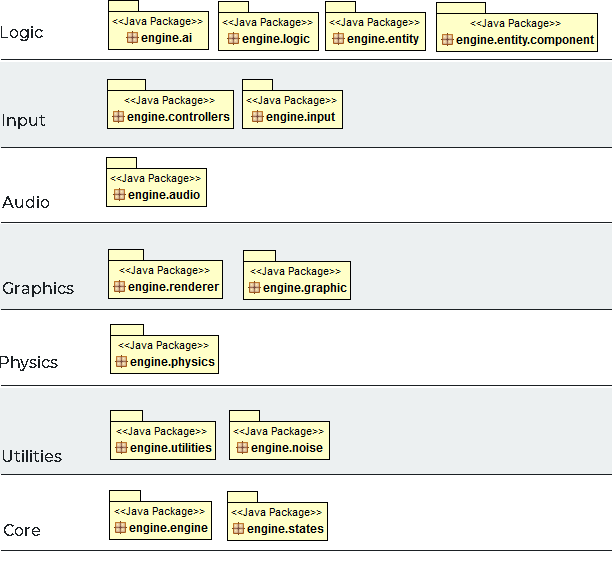
\includegraphics[width=\textwidth]{imagens/engineLayers.png}
	\caption{Pacotes da engine Narval divididos em camadas
    \label{fig:arquitetura}}
\end{figure}

\section{\textit{Game Loop}}
Game loop é o núcleo da arquitetura de uma engine. É neste loop que todos os subsistemas da engine são chamados e  executados, como a renderização, detecção e resolução de colisões, áudio e muitos outros \cite{GameEngineArchitecture}. Por se tratar de uma simulação em tempo real, onde a tela inteira deve ser atualizada em uma quantidade muito alta de vezes, é fundamental que tudo seja executado o mais rápido possível e em tempo constante para que o usuário tenha uma experiência fluída e dinâmica.

Portanto, o tempo demanda um papel chave neste sistema e deve ser cuidadosamente levado em consideração para que não haja quaisquer gargalos que deturpem a fluidez e experiência final do usuário. A estrutura mais simples de um game loop é composta como se segue:

\begin{lstlisting}[caption={Estrutura básica do Game Loop}, label={alg:gameloopbasico}]
while(true) {
	update();
	render();
}
\end{lstlisting}


O algoritmo \ref{alg:gameloopbasico} sendo executado ao longo do tempo é representado pela Figura~\ref{fig:gameloopbasico}.
Cada execução do método \texttt{render} significa o desenho de uma imagem na tela e a quantidade total de imagens desenhadas ao longo de um segundo é representada pela unidade de medida FPS (\textit{Frames per second}). Cada execução do método \texttt{update} significa um passo no tempo do jogo (\textit{timestep}). Da mesma forma que o relógio move-se em tiques de um segundo em um segundo, o tempo do jogo avança em tiques de \texttt{update} em \texttt{update}.

\begin{figure}[H]
	\centering
	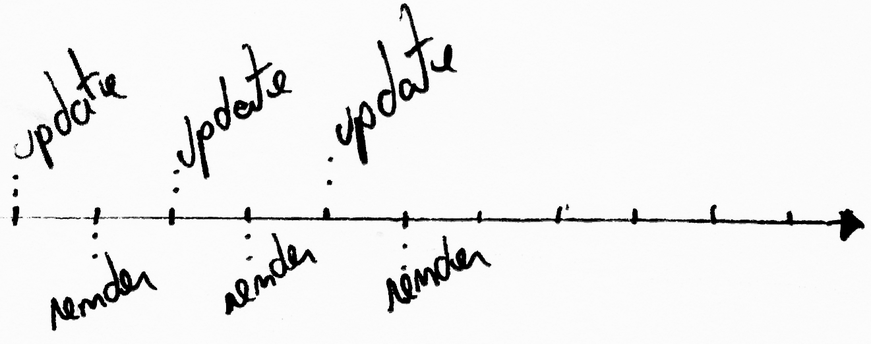
\includegraphics[width=28em]{imagens/ilu1_small.png}
	\caption{Execução do game loop básico ao longo do tempo\label{fig:gameloopbasico}}
\end{figure}




\section{Sistema de atualização}
O sistema de atualização é responsável por controlar o aspecto lógico da engine. Nele ocorrem todos os cálculos relativos a movimentação dos objetos, colisões, inteligência artificial e outros. Sendo assim, é um sistema composto de outros sistemas, cada um rodando com uma taxa de atualização específica e não obrigatoriamente atrelados ao FPS.

\subsection{Timestep fixo}
Sistemas de atualização com timestep fixo são aqueles que estavam diretamente atrelados ao FPS e eram utilizados em jogos antigos \cite{GameEngineArchitecture}. As unidades de medida de tempo eram diretamente atreladas ao FPS tal que, se uma máquina fosse capaz de rodar o jogo a 30 FPS e outra a 60 FPS, na segunda máquina o jogo daria impressão de estar duas vezes mais rápido ou duas vezes mais lento dependendo do valor fixado para o timestep. Isso acontecia por que os jogos eram desenvolvidos para plataformas específicas e, sabendo em qual taxa de FPS o jogo iria rodar, era fácil delimitar um timestep fixo.

Entretanto, conforme as máquinas se tornaram mais potentes e o mercado passou a oferecer mais opções de hardware, logo a indústria estava produzindo jogos para um SO com múltiplas possibilidades de hardware. Essa gama de computadores com capacidades de processamento distintas gerou o problema descrito acima. Por exemplo, seja uma máquina \texttt{MA} capaz de rodar o jogo a 30 FPS e uma máquina \texttt{MB} capaz de rodar a 60 FPS, sendo a máquina \texttt{MA} o alvo do projeto. Se um personagem deveria mover-se a  300 pixels por segundo, logo 10 pixels por frame ($300 px/ 30 FPS$), na máquina \texttt{MB} ele estaria se movendo a 600 pixels por segundo pois ao dobrar o \textit{FPS} dobra-se a quantidade de vezes que o método \texttt{update} é chamado, e portanto, o personagem passa a mover-se a 600 pixels por segundo ($60 FPS * 10 px p/ frame$). Isso acontece por que antigamente o jogo era projetado para rodar numa máquina cuja capacidade de FPS seria $x$ e a variável $\Delta t$, que representa o tempo transcorrido entre um frame e outro, seria o inverso de $x$, ou simplesmente o inverso da frequência, o período $1/x$. A partir disso a posição do objeto era calculada efetuando-se $pos(i) = pos(i-1) + velPerFrame$ e como $\Delta t$ é um valor fixo dado por $1/x$ (baseado num FPS de $x$), tem-se que em um computador mais potente, o tempo transcorrido entre um frame e outro é menor e portanto o período aumenta. Como o valor foi pré-calculado para uma máquina alvo, ele não diminui na máquina mais potente e acaba sendo somado mais vezes, resultando em uma velocidade maior que a originalmente desejada. Esse problema pode ser facilmente representado por uma série.

\noindent
Em um PC capaz de rodar a 30FPS: $$\sum_{n=1}^{30} 10px = 300 px/s$$

\noindent
Em um PC capaz de rodar a 60FPS: $$\sum_{n=1}^{60} 10px = 600 px/s$$

\noindent
Sendo assim, a estrutura do game loop com timestep fixo seria:
\begin{lstlisting}[caption=Game Loop com timestep fixo]
public static final float dt = 1f/30f;

while(true) {
	update(dt);
	render();
}
\end{lstlisting}
E pode ser representado pela figura:
\begin{figure}[H]
	\centering
	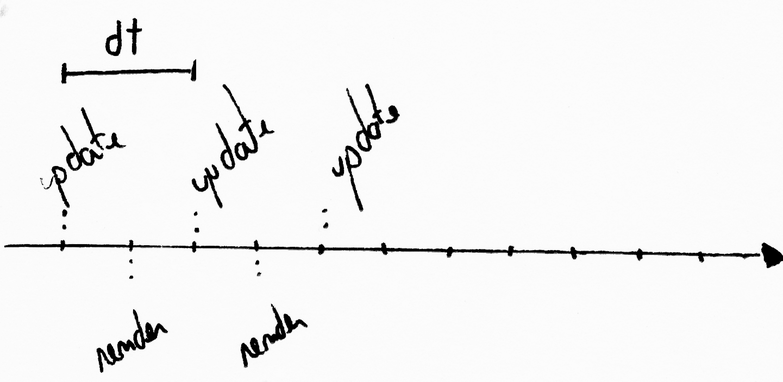
\includegraphics[width=28em]{imagens/ilu2_small.png}
	\caption{Execução do game loop com timestep fixo ao longo do tempo}
\end{figure}

\subsection{Timestep variável}
Para que a taxa de atualização $\Delta t$ seja dinâmica ao invés de fixa, ela precisa ser independente do FPS. Isso é possível medindo-se quanto tempo transcorre entre um frame e outro. Dessa forma o game loop fica definido como se segue:

\begin{lstlisting}[caption=Game loop com timestep variável]
private long lastFrame;
private long dt;
		
while(true) {
	long currentFrame = System.nanoTime(); 
	dt = currentFrame - lastFrame;
	lastFrame = currentFrame;
	
	update(dt);
	render();
}
\end{lstlisting}
Esse código é representado pela figura:
\begin{figure}[H]
	\centering
	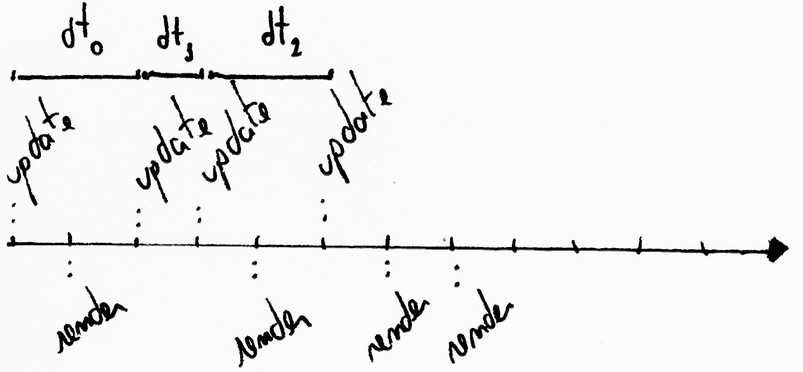
\includegraphics[width=28em]{imagens/ilu3_small.png}
	\caption{Execução do game loop com timestep variável ao longo do tempo}
\end{figure}

Embora tenha-se resolvido o problema anterior de dois computadores com capacidades diferentes de processamento, o sistema ainda não é ideal. A falha está no fato de utilizar o $\Delta t$ anterior ao frame atual. Se o tempo passado entre um frame e outro for muito grande, ou seja, se houver um pico de performance, será avançado um tempo muito grande e um passo do personagem que era para ser $10 pixels$, passa a ser $10px + atraso$. Isso gera um efeito chamado de \textit{stuttering} e é percetível ao jogador, pois atrapalha a fluidez da movimentação. Isso também traz consequências na lógica do programa. Um objeto que deveria percorrer 10 pixels por timestep, ao percorrer mais em um único timestep poderia, por exemplo, estar ignorando uma colisão que iria ocorrer entre o ponto atual e o próximo.
\begin{figure}[H]
	\centering
	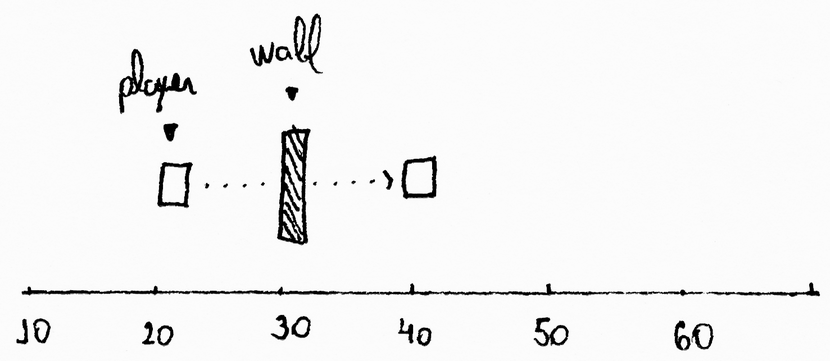
\includegraphics[width=28em]{imagens/ilu4_small.png}
	\caption{Objeto ignorando colisão devido um timestep muito grande}
\end{figure}
 Não só isso, mas um timestep variável traz toda uma complicação com a depuração. Ao introduzir um fator não determinístico no processo, pode ser que seja impossível reproduzir um cenário de bug para efetuar seu diagnóstico e correção. 

\subsection{Timestep semi-fixo}
Um game loop com timestep semi-fixo tenta trazer o melhor dos dois mundos. Isso é possível usando um $\Delta t$ fixo para cada chamada do método update e, quando o sistema demorar mais que o $\Delta t$ fixado, faz-se a recuperação do mesmo chamando o método \texttt{update} quantas vezes necessário.
Isso é fácil visualizar quando demonstrado em código:

\begin{lstlisting}[caption={Game Loop com timestep semi-fixo}]
private long lastFrame;
private long accumulator = 0;
private long dt;
public static final long ONE_SECOND_IN_NANOSECONDS = 10^9;
public static final long STEPS_PER_SECOND = 30;
public static final long FIXED_DT = ONE_SECOND_IN_NANO/STEPS_PER_SECOND;
			
while(true) {
	long currentFrame = System.nanoTime(); 
	dt = currentFrame - lastFrame;
	lastFrame = currentFrame;
	accumulator += dt;
	
	while (accumulator >= FIXED_DT){
    	update(dt);
    	accumulator -= FIXED_DT;
 	 }
 			 
	render();
}
\end{lstlisting}

É importante ter cuidado com o valor escolhido para o \texttt{FIXED_DT} (timestep). Se o timestep for menor que o tempo que se leva para processar o método \texttt{update} o sistema nunca irá recuperar seu atraso, tendo um acumulador que sempre cresce e nunca fica próximo de zerar \cite{GameProgrammingPatterns}.
O sistema de timestep semi-fixo é demonstrado pela ilustração:
\begin{figure}[H]
	\centering
	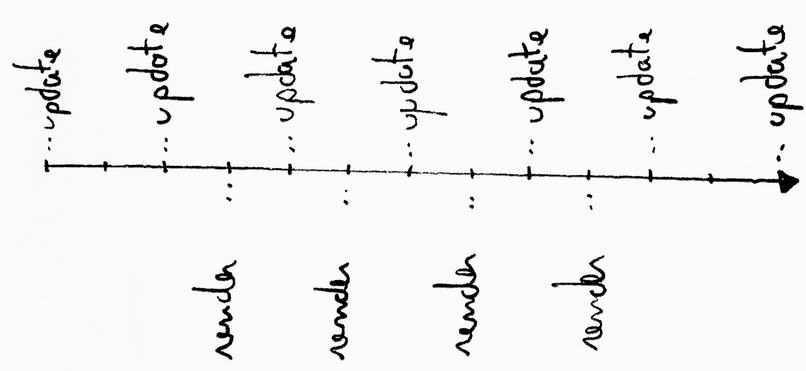
\includegraphics[width=28em]{imagens/ilu6_small.png}
	\caption{Execução do game loop com timestep semi-fixo ao longo do tempo}
\end{figure}
O problema em que o processamento do método update é maior que o $\Delta t$ é mostrado na figura seguinte. Note que o valor de $dt_0$ é maior que o $\Delta t$ fixado e o sistema só tende a piorar ao longo do tempo, acumulando cada vez mais atraso nos valores de $dt$ e nunca se recuperando.
\begin{figure}[H]
	\centering
	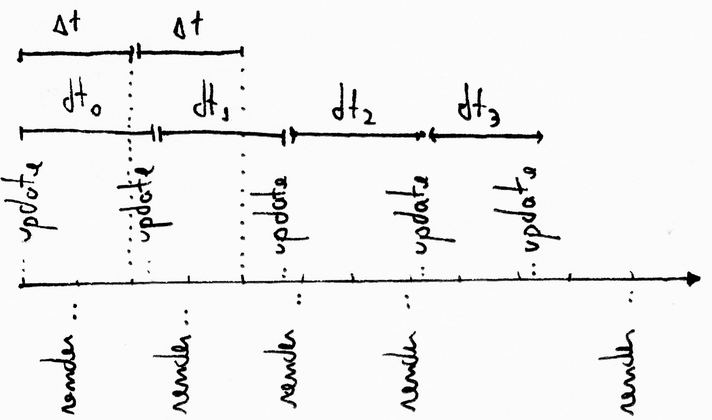
\includegraphics[width=28em]{imagens/ilu8_small.png}
	\caption{Método \texttt{update} com tempo de processamento maior que o $\Delta t$}
\end{figure}
 
\section{Sistema de renderização}
É neste sistema que todos os objetos visíveis na tela são desenhados. Esse sistema é executado diversas vezes e em rápida sucessão durante um segundo através do método \texttt{render}, criando uma ilusão de movimento. Esse processo se inicia no processador e termina na placa gráfica acontecendo quantas vezes a máquina conseguir ou quantas vezes o usuário desejar configurar. Os valores mais comuns para fixar o FPS são atrelados à frequência do monitor que, atualmente, variam de 30 Hz até 144 Hz e para todos os efeitos Hertz é uma medida equivalente ao FPS \cite{GameEngineArchitecture}.

\subsection{Interpolação Linear} 
\label{subsec:interpoLinear}
Com o timestep definido ainda é necessário mais um procedimento para que o sistema renderize objetos em movimento de forma suave. O efeito de \textit{stuttering} pode ser causado tanto pelo aspecto lógico, através dos picos de performance, quanto pelo simples fato de que não se possui total controle sobre como o SO gerencia a aplicação. Não é possível garantir uma taxa de atualização e renderização intercalada e perfeita. Haverá momentos que depois de um único \texttt{update} o método \texttt{render} será chamado várias vezes se processado em um tempo menor que o $\Delta t$ e, sem nenhum tratamento, este efeito também causa \textit{stuttering}. Ao chamar o método \texttt{render} consecutivamente e não atualizar a posição do objeto em cada chamada, o usuário tem a impressão de um sistema engasgado com movimento não fluído.
Para resolver este último problema é necessário realizar uma interpolação linear entre a posição anterior e atual do objeto, tornando seu movimento suave. Esse efeito pode ser visualizado nas figuras \ref{fig:renderSemInterpolacao} e \ref{fig:renderComInterpolacao} onde um objeto move-se 10 pixels por segundo. Na primeira figura a função \texttt{render} é chamada sem nenhum tratamento e portanto renderiza o objeto no mesmo lugar até que sua posição seja atualizada no próximo \texttt{update}. Já na segunda figura, é renderizada a interpolação da posição desse objeto, tornando seu movimento muito mais suave para o usuário.
\begin{figure}[H]
	\centering
	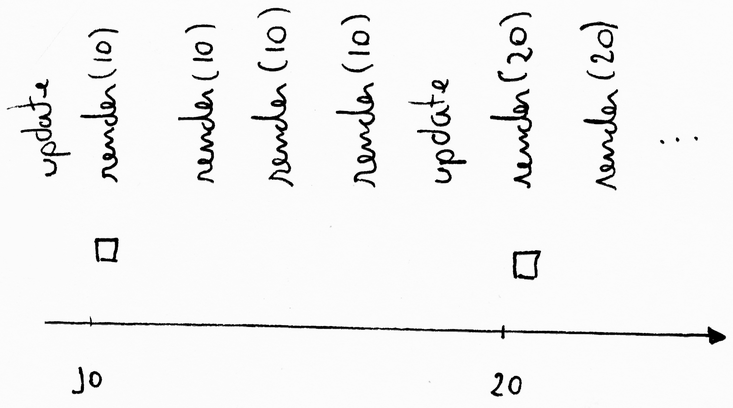
\includegraphics[width=28em]{imagens/ilu7_small.png}
	\caption{Renderização sem interpolação
	\label{fig:renderSemInterpolacao}}
\end{figure}
\begin{figure}[H]
	\centering
	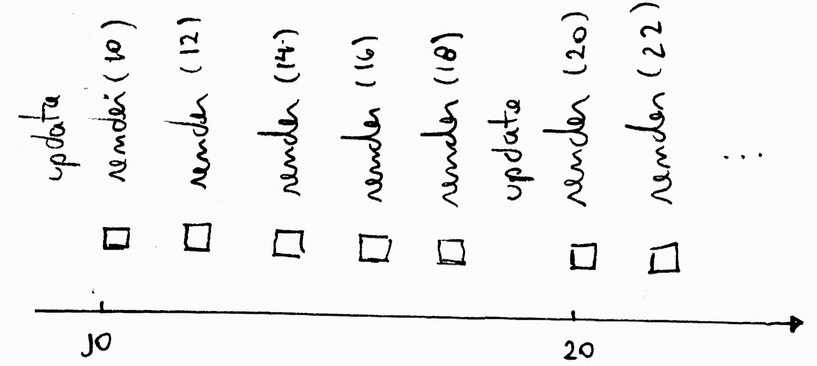
\includegraphics[width=28em]{imagens/ilu5_small.png}
	\caption{Renderização sem interpolação
	\label{fig:renderComInterpolacao}}
\end{figure}

\noindent
O código final do game loop, para um sistema com timestep semi-fixo e com interpolação linear fica como se segue:
\begin{lstlisting}[caption=Game Loop com timestep semi-fixo e interpolação linear]
		long lastFrame;
		long accumulator = 0;
		long dt;
		public static final long ONE_SECOND_IN_NANOSECONDS = 10^9;
		public static final long STEPS_PER_SECOND = 30;
		public static final long FIXED_DT = ONE_SECOND_IN_NANO/STEPS_PER_SECOND;
		
		
		while(true) {
			long currentFrame = System.nanoTime(); 
			dt = currentFrame - lastFrame;
			lastFrame = currentFrame;
			accumulator += dt;
	
			while (accumulator >= FIXED_DT){
    			update(dt);
    			accumulator -= FIXED_DT;
 			 }
 			 
			long interpolationFactor = accumulator / FIXED_DT; 			 
 			 
			render(interpolationFactor);
		}
\end{lstlisting}
Dentro da função \texttt{render} o fator de interpolação é utilizado na seguinte fórmula para obter a posição onde o objeto deve ser renderizado:

\begin{quote}
$renderPosition$ = $currentPosition * interpolationFactor$ + $previousPosition * (1 - interpolationFactor)$
\end{quote}

\section{API gráfica OpenGL}
OpenGL é a API encarregada da comunicação com a GPU. Através dela são realizadas todas as chamadas de função responsáveis por desenhar objetos na tela. Cada Engine deve utilizar uma API dependendo da plataforma na qual o produto final será disponibilizado. Por exemplo, para um sistema mobile existe a API OpenGL ES, para Windows tem-se a OpenGL, DirectX etc. De certa forma, as APIs gráficas compõem essencialmente o sistema de renderização.  

\subsection{Core-profile e Immediate mode}
Immediate mode (legado) é o modo antigo de se operar com OpenGL e foi depreciado em 2008 com o lançamento da versão 3.0 \cite{OpenGLHistory}. Hoje ele é substituído pelo modo \textit{Core-profile}. No modo antigo as funções eram mais fáceis de usar, com muitas funcionalidades já abstraídas pela API. Entretanto, por serem funções abstraídas elas forneciam uma menor flexibilidade de controle sobre como o OpenGL  operava e eram também ineficientes~\cite{LearnOpenGL}. Com o passar do tempo e uma demanda dos desenvolvedores por maior flexibilidade a API foi depreciada e substituída pelo modo \textit{Core-profile}, em que tem-se muito mais controle sobre como o OpenGL opera. Entretanto, isso vem ao custo de uma maior curva de aprendizagem e complexidade de implementação.

\subsection{State Machine}
O OpenGL funciona como uma grande máquina de estados, possuindo uma enorme coleção de variáveis que definem como  operar no estado vigente. Chamam-se as funções para configurar o estado atual, passar dados (coordenadas geográficas, cores e outras informações) ou alterar modos de operação. Um desses estados é o \textit{rendering state} cujo divisão é feita em várias categorias como: \textit{color}, \textit{texturing}, \textit{lighting} e assim por diante. O \textit{rendering state} é manipulado pelas funções \texttt{glEnable(feature)} e \texttt{glDisable(feature)} que recebem como argumento um \texttt{enum} indicando qual o atributo que se deseja habilitar.

\subsection{Hello window}
A primeira etapa necessária para usar o OpenGL é criar um contexto e uma janela onde renderizar. O processo de criação da janela é específico de cada SO e faz-se necessário o uso de outra API para abstrair esse passo. A biblioteca a ser utilizada será a \texttt{GLFW}. O código a seguir demonstra esse processo:
\begin{lstlisting}[caption=Inicialização da janela e contexto OpenGL]
public class Window {
	private int width;
	private int height;
	private Vec2 size;
	private String name;
	private long id;
	
	public Window(int width, int height, String name) {
		this.width = width;
		this.height = height;
		this.name = name;
		size = new Vec2(width,height);
	}
	
	public void init() {
		if (!glfwInit()) 
			System.err.println("Could not initialize GLFW.");

		glfwWindowHint(GLFW_CONTEXT_VERSION_MAJOR, 3);
		glfwWindowHint(GLFW_CONTEXT_VERSION_MINOR, 3);
		glfwWindowHint(GLFW_OPENGL_PROFILE, GLFW_OPENGL_CORE_PROFILE);
		glfwWindowHint(GLFW_RESIZABLE, GL_FALSE);

		id = glfwCreateWindow(width, height, name,  NULL,  NULL);
		glfwMakeContextCurrent(id);

		glfwSetWindowPos(id, 2000, 60);
		glfwShowWindow(id);
		GL.createCapabilities();
		glfwSwapInterval(1); //VSYNC

		glViewport(0,0, width, height);
		glEnable(GL_CULL_FACE);
		glEnable(GL_BLEND);
		glBlendFunc(GL_SRC_ALPHA, GL_ONE_MINUS_SRC_ALPHA);
	}
}
\end{lstlisting}
Primeiramente inicia-se o GLFW através da chamada \texttt{glfwInit()}. Em seguida usa-se a função \texttt{glfwWindowHint(hint, value)} para adicionar atributos a janela, sendo o primeiro argumento o nome do atributo (de tipo \texttt{enum}) e o segundo argumento o valor que se deseja atribuir. No exemplo definido para a função \texttt{init} acima, foram inseridos os atributos \texttt{GLFW_CONTEXT_VERSION_MAJOR} e  \texttt{GLFW_CONTEXT_VERSION_MINOR} indicando qual a versão mínima para rodar a aplicação. Essa versão é representada no formato [MAJOR].[MINOR] e, portanto, neste cenário a versão é 3.3. O atributo \texttt{GLFW_OPENGL_PROFILE} altera entre o modo core profile e immediate mode (legado). Cria-se então a janela com o método \texttt{glfwCreateWindow(width, height, title, monitor, share)} e usa-se o id retornado para torná-lo contexto vigente com
\linebreak \texttt{glfwMakeContextCurrent(id)}. A função \texttt{glfwShowWindow(id)} é chamada para tornar essa janela visível ao usuário. Para utilizar o OpenGL e criar seu contexto é necessário chamar \texttt{GL.createCapabilities}. A partir deste ponto o OpenGL pode ser utilizado normalmente. A função \texttt{glViewport(0,0, width, height)} define o tamanho do viewport ou, simplesmente, o tamanho da área de renderização e é geralmente usado como tendo o mesmo tamanho da janela.

\subsection{OpenGL Pipeline}
No intuito de desenhar objetos na janela, é necessário abordar dois elementos do OpenGL: \textit{buffer objects} e \textit{pipeline}. Os \textit{buffer objects} são estruturas responsáveis por transmitir e encapsular os dados a serem enviados para a GPU. Existem 9 tipos de objetos e estes são divididos em duas categorias~\cite{OpenGLObject}:

\begin{enumerate}
\item \textbf{Regular objects}: objetos dessa categoria contêm dados.
\begin{itemize}
\item Buffer object
\item RenderBuffer object
\item Texture object
\item Query object
\item Sampler object
\end{itemize}
\item \textbf{Container objects}:  objetos dessa categoria servem apenas de containers para transportar os elementos da lista anterior (\textit{regular objects}). 
\begin{itemize}
\item Framebuffer object
\item Vertex Array object
\item Transform Feedback object
\item Program pipeline object
\end{itemize}
\end{enumerate}

Neste primeiro momento será abordado o \textit{Vertex Buffer Object} (VBO) e \textit{Vertex Array Object} (VAO). A fim de desenhar um objeto na tela faz-se necessário enviar a GPU os vértices que o compõem. O \textit{pipeline} recebe como entrada uma série de vértices, os processa e transforma em pixels 2D na tela \cite{LearnOpenGL}. Cada etapa do \textit{pipeline} recebe como entrada a saída da etapa anterior.

As etapas customizáveis do \textit{pipeline} são processadas por pequenos programas chamados \textit{shaders}. Esses programas são escritos em GLSL pelo desenvolvedor da aplicação e ficam alojados na GPU, sendo altamente paralelizáveis e especializados. A seguir tem-se uma representação simplificada do processo que ocorre no pipeline para desenhar um pequeno triângulo.

\begin{figure}[H]
	\centering
	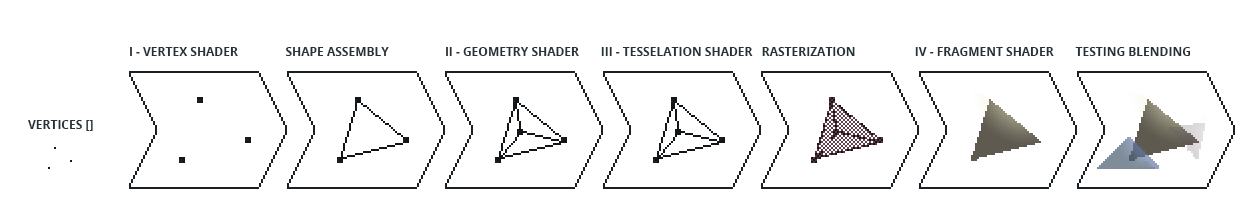
\includegraphics[width=\textwidth]{imagens/openglpipeline.png}
	\caption{Etapas do pipeline  \label{fig:pipeline}}
\end{figure}

Na etapa I o \textit{vertex shader} é responsável, principalmente, por receber um único vértice e transformar sua coordenada cartesiana de um sistema para outro. Por exemplo, as coordenadas finais desse objeto vão mudar conforme a câmera se movimenta no espaço. É também necessário converter a posição local do objeto para a sua posição global no ambiente. Esses e outros processos serão melhor abordados no capítulo sobre Sistemas de Coordenadas.

Na etapa do \textit{shape assembly} o OpenGL monta todos os vértices recebidos como entrada na primitiva selecionada para renderização. São algumas delas: \textit{GL_POINTS}, \textit{GL_LINES} e \textit{GL_TRIANGLES}.

A etapa do \textit{geometry shader} recebe como entrada a primitiva de saída do \textit{shape assembly}. A partir desses vértices o \textit{geometry shader} é capaz de gerar novos vértices e formar novas primitivas. No exemplo da Figura \ref{fig:pipeline} ele recebe um triângulo e cria um novo vértice no centro, resultando em 3 sub-triângulos.

O \textit{tesselation shader} é altamente especializado em subdividir uma primitiva em outras muito menores. Essa função é útil para, por exemplo, detalhar objetos mais próximos da tela e generalizar objetos mais distantes reduzindo sua quantidade de vértices.

A etapa de \textit{rasterization} processa a saída do \textit{tesselation shader} e converte todas essas informações em coordenadas 2D na tela ou, simplesmente, em pixels na tela. Esses pixels são então repassados como fragmentos para o \textit{fragment shader}.

Na penúltima etapa do pipeline, o \textit{fragment shader} processa todos os fragmentos para dar aos pixels sua cor final. É neste estágio que todos os efeitos visuais são aplicados como, por exemplo, a iluminação.

Por fim, no último estágio é aplicado o \textit{blending} e  outros testes. \textit{Blending} nada mais é do que calcular o quanto a transparência de um objeto afeta outro. No exemplo da Figura \ref{fig:pipeline} isso é representado pelos dois triângulos menores que afetam a cor final do triângulo maior aonde estes se sobrepõem. Neste estágio também são realizados os testes de \textit{depth} e \textit{stencil}.

\subsection{Vertex Array Object e Vertex Buffer Object}
Todo objeto no OpenGL é manipulado através de seu ID. Portanto, faz-se necessário gerar o ID do VAO e VBO chamando as funções \texttt{glGenVertexArrays()} e \linebreak \texttt{glGenBuffers()}. Após gerados os IDs vincula-se esse \textit{data object} como o vigente através da função \texttt{glBindBuffer}\texttt{(type, id)} e insere-se os dados nele através da função \texttt{glBufferData(type, data, draw_type)}. Para o \textit{object container} o processo é similar. Vincula-se o VAO com \texttt{glBindVertexArray(id)} e habilita-se a localização do atributo do vértice no \textit{vertex shader} através da função \texttt{glEnableVertexAttribArray(index)}. Por fim, configura-se como cada vértice deve ser interpretado, nesta situação como um bloco de 4 floats, sendo 2 deles as posições $x$ e $y$ do objeto e os dois últimos a posição $x$ e $y$ da textura que compõem esse objeto. Essa configuração é feita pela função \texttt{glVertexAttribPointer(index, size, type, normalized, stride, pointer)}.

\begin{lstlisting}[caption=Inicialização do VBO e VAO, label={alg:initVBOVAO}]
private void init() {
	float vertices [] = {
			//Pos	//Texture
			0,	1,	0,	1f,
			1,	0,	1f,	0,
			0,	0,	0,	0,
			
			0,	1,	0,	1f,
			1,	1,	1f,	1f,
			1,	0,	1f,	0
	};
	
	int quadVAO = glGenVertexArrays();
	int VBO = glGenBuffers();
	
	glBindBuffer(GL_ARRAY_BUFFER, VBO);
	glBufferData(GL_ARRAY_BUFFER, BufferUtilities.createFloatBuffer(getVertices(3)), GL_STATIC_DRAW); 
	
	glBindVertexArray(quadVAO);
	glEnableVertexAttribArray(0);
	glVertexAttribPointer(0, 4, GL_FLOAT, false, Float.BYTES * 4, 0);
	
	glBindBuffer(GL_ARRAY_BUFFER, 0);
	glBindVertexArray(0);
}
\end{lstlisting}

A variável \texttt{vertices} contém os vértices no espaço local do objeto. Essas coordenadas são então posteriormente processadas no vertex shader e transformadas em coordenadas globais.
\begin{figure}[H]
	\centering
	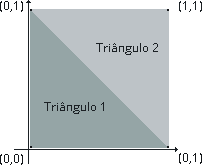
\includegraphics[width=24em]{imagens/tringulosCompondoQuad.png}
	\caption{Dois triângulos em coordenadas locais normalizadas que juntos formam um quadrado}
\end{figure}

\subsection{OpenGL Shading Language (GLSL)}
???

\subsection{Vertex e Fragment shader}
Após a geração do objeto, configuração e posterior transferência dos dados para a GPU, pode-se iniciar o processo de manipulação desses dados no \textit{shader}. Como ilustrado na Figura~\ref{fig:pipeline}, o primeiro shader do pipeline é o \textit{vertex shader}. Todo código escrito no shader é iniciado com a versão do OpenGL. Neste caso, a versão utilizada é a 3.3 e o modo, que deve ser explicitamente citado, é o modo \textit{core profile}.
O index layout, onde o dado é recebido no shader, para este exemplo é 0 e usa o formato de um vetor de 4 floats. Dessa forma a primeira parte do código fica:
\begin{lstlisting}[caption=Vertex shader header]
#version 330 core
layout (location = 0) in vec4 vertex; //xy Obj coord
									  //zw Texture coord
\end{lstlisting}

Definido o cabeçalho agora é necessário dizer quais serão as saídas do shader, ou simplesmente, seu retorno que servirá de entrada para a próxima etapa do pipeline. Isso é feito usando-se a palavra reservada \texttt{out} seguida do tipo e nome da variável. Ainda neste escopo são definidas as variáveis do tipo \texttt{uniform}, que funcionam como variáveis globais e podem ser acessadas em qualquer shader. Em seguida declara-se a função main, responsável pela manipulação destes dados.

 \begin{lstlisting}[caption=Vertex shader simples]
#version 330 core
layout (location = 0) in vec4 vertex; //xy position
									 //zw Tex coord

out vec2 TexCoords;

uniform mat4 model;
uniform mat4 projection;
uniform mat4 camera;

uniform vec2 flip;

void main(){
	TexCoords = vertex.zw;
	gl_Position = projection * camera * model *  vec4(vertex.xy, 0.0 , 1.0);
}
\end{lstlisting}

Esse shader recebe um vetor de 4 floats contendo as coordenadas $x$ e $y$ do objeto e as coordenadas $z$ e $w$ da textura. As coordenadas da textura são passadas adiante para o fragment shader através da variável \texttt{TexCoords} e as coordenadas do vértice são multiplicadas pelas matrizes de projeção, câmera e modelo para obter as coordenadas globais. O resultado dessa multiplicação é armazenado na variável global do openGL chamada \texttt{gl_Position}.

A próxima etapa a ser abordada é a do fragment shader. Para a construção desse primeiro exemplo a única manipulação que será feita nos fragmentos é a renderização da textura. Com a entrada da etapa anterior (vertex shader) extrai-se da textura contida na variável \texttt{image} a fatia desejada usando as coordenadas em TexCoords (linha 5). Esse resultado é então enviado para a última etapa usando-se a variável \texttt{out vec4 color}.

 \begin{lstlisting}[caption=Fragment shader simples]
#version 330 core
in vec2 TexCoords;
out vec4 color;

uniform sampler2D image;

void main(){
	vec4 imgTex =  texture(image, TexCoords).xyzw;
	color = imgTex;
}
\end{lstlisting}

\begin{figure}[H]
	\centering
	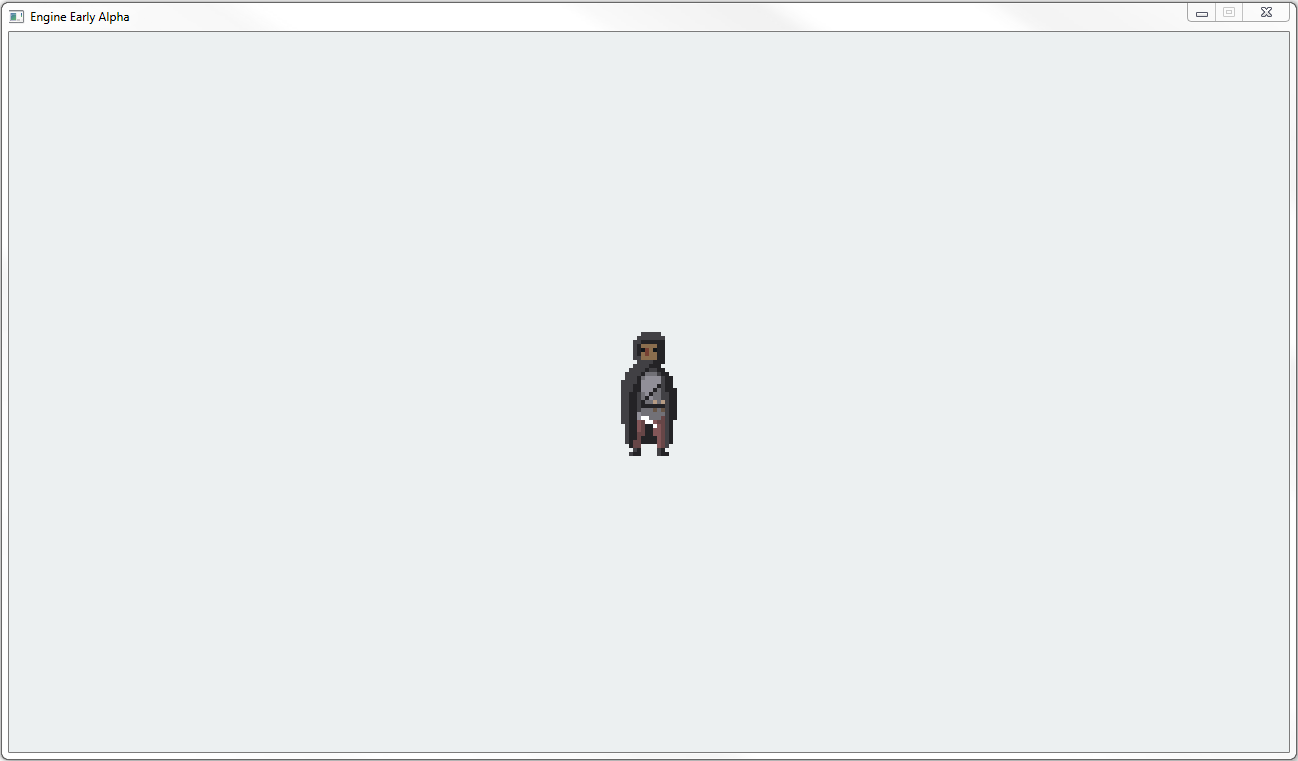
\includegraphics[width=\textwidth]{imagens/helloShader.png}
	\caption{Resultado obtido com dois shaders simples}
\end{figure}

\subsection{Compilando o shader em um programa}
Com o código dos shaders salvos em arquivo é necessário compilá-los e envia-los a GPU antes de poderem ser efetivamente usados. Assim como qualquer objeto no OpenGL o primeiro passo é gerar um ID para referenciá-lo. Esse processo é feito chamando \texttt{glCreateShader(type)}. Os tipos possíveis de shader são aqueles demonstrados e numerados de I a IV na figura \ref{fig:pipeline}. Portanto, os valores possíveis são: \texttt{GL_COMPUTE_SHADER},  \texttt{GL_VERTEX_SHADER},  \texttt{GL_TESS_CONTROL_SHADER},\linebreak  \texttt{GL_TESS_EVALUATION_SHADER},  \texttt{GL_GEOMETRY_SHADER}, e  \texttt{GL_FRAGMENT_SHADER}~\cite{openGLShaderCompilation}. Com o objeto criado atribui-se o código ao objeto e o mesmo é compilado a partir das funções \texttt{glShaderSource(id, code)} e \texttt{glCompileShader(id)}. Para checar se a compilação foi realizada com sucesso chama-se a função \texttt{glGetShaderi(id, GL_COMPILE_STATUS)}. Se o retorno for 0 (FALSE) não houve erros. Caso contrário, a função \texttt{glGetShaderInfoLog(id)} retorna a mensagem de erro, que pode ser posteriormente impressa na tela.

 \begin{lstlisting}[caption=Processo de compilação do shader]
	int vertexShader = glCreateShader(GL_VERTEX_SHADER);
	glShaderSource(vertexShader, vertexSource);
	glCompileShader(vertexShader);
	
	int success = glGetShaderi(vertexShader, GL_COMPILE_STATUS);
			
	if(success==0) {
		String log = glGetShaderInfoLog(vertexShader);
		System.err.println(log);
	}
\end{lstlisting}

Tendo os shaders necessários compilados agora é necessário criar um programa. Essa etapa segue um padrão baseado no processo de dois estágios para compile/link usada nos programas escritos em C e C++. O código fonte é primeiro servido ao compilador, produzindo um object file. Para obter o executável final é necessário encadear um ou mais object files juntos. Com o programa criado e os shaders encadeados a ele é possível utilizar todos esses shaders com apenas uma chamada do programa.

 \begin{lstlisting}[caption=Processo de criação e link de um programa]
	int id = glCreateProgram();
	glAttachShader(id, vertexShader);
	glAttachShader(id, fragmentShader);
	glLinkProgram(id);
	
	int success = glGetProgrami(id, GL_LINK_STATUS);
			
	if(success==0) {
		String log = glGetProgramInfoLog(id);
		System.err.println(log);
	}
\end{lstlisting}

Os shaders uma vez encadeados podem ser removidos para liberar espaço usado a função \texttt{glDeleteShader(id)}.

\subsection{Uniforms}

Existem duas formas de se enviar dados para um shader, através dos objects e através das variáveis globais definidas como \texttt{uniform}. Para alocar um valor nessas variáveis é necessário primeiro usar o programa que contém este shader com a função \texttt{glUseProgram(id)} e em seguida usar uma das funções da família \texttt{glUniform...()}. O formato dessas funções é glUniform+quantity+type. Por exemplo, para atribuir um valor a uma váriavel float utiliza-se \texttt{glUniform1f (glGetUniformLocation (programID, variableName), value)}, para um vetor de 3 floats usa-se \texttt{glUniform3f(glGetUniformLocation (programID,variableName), x, y, z)}, para uma matriz 4 por 4  \texttt{glUniformMatrix4fv(glGetUniformLocation (programID,variableName), false, BufferUtilities.createFloatBuffer(m))} e assim por diante.
Dessa forma a classe final do Shader fica:

 \begin{lstlisting}[caption=Shader class]
public class Shader {
	private int id;
	
	public Shader use() {
		glUseProgram(this.id);
		return this;
	}
	public int getId() {
		return id;
	}

	public void compile(String vertexSource, String fragmentSource, String geometrySource) {
		int vertexShader, geometryShader = 0, fragmentShader;
		
		vertexShader = glCreateShader(GL_VERTEX_SHADER);
		glShaderSource(vertexShader, vertexSource);
		glCompileShader(vertexShader);
		checkCompileErrors(vertexShader, "VERTEX");
		
		fragmentShader = glCreateShader(GL_FRAGMENT_SHADER);
		glShaderSource(fragmentShader, fragmentSource);
		glCompileShader(fragmentShader);
		checkCompileErrors(fragmentShader, "FRAGMENT");
		
		if(geometrySource!=null) {
			geometryShader = glCreateShader(GL_GEOMETRY_SHADER);
			glShaderSource(geometryShader, geometrySource);
			glCompileShader(geometryShader);
			checkCompileErrors(fragmentShader, "GEOMETRY");
		}
		
		id = glCreateProgram();
		glAttachShader(id, vertexShader);
		if(geometrySource!=null)
			glAttachShader(id, geometryShader);
		glAttachShader(id, fragmentShader);
		glLinkProgram(id);
		checkCompileErrors(id, "PROGRAM");
		
		glDeleteShader(vertexShader);
		glDeleteShader(fragmentShader);
		if(geometrySource!=null)
			glDeleteShader(geometryShader);
	}
	
	private void checkCompileErrors(int object, String type) {
		int success;
		String log;
		
		if(type!="PROGRAM") {
			success = glGetShaderi(object, GL_COMPILE_STATUS);
			
			if(success==0) {
				log = glGetShaderInfoLog(object);
				System.err.println(log);
			}
				
		}else {
			success = glGetProgrami(object, GL_LINK_STATUS);
			
			if(success==0) {
				log = glGetProgramInfoLog(object);
				System.err.println(log);
			}
				
		}
	}
	
	public void setFloat(String name, float value) {
		glUniform1f(glGetUniformLocation(id,name), value);
	}
	
	public void setInteger(String name, int value) {
		glUniform1i(glGetUniformLocation(id,name), value);
	}
	
	public void setVec2(String name, float x, float y) {
		glUniform2f(glGetUniformLocation(id,name), x,y);
	}
	
	public void setVec2(String name, Vec2 pos) {
		glUniform2f(glGetUniformLocation(id,name), pos.x, pos.y);
	}
	
	public void setVec3(String name, float x, float y, float z) {
		glUniform3f(glGetUniformLocation(id,name), x,y,z);
	}
	
	public void setVec3(String name, Vec3 pos) {
		glUniform3f(glGetUniformLocation(id,name), pos.x, pos.y, pos.z);
	}
	
	public void setVec4(String name, float x, float y, float z, float w) {
		glUniform4f(glGetUniformLocation(id,name), x, y, z, w);
	}
	
	public void setVec4(String name, Vec4 pos) {
		glUniform4f(glGetUniformLocation(id,name), pos.x, pos.y, pos.z, pos.w);
	}

	public void setMat4(String name, Mat4 m) {
		glUniformMatrix4fv(glGetUniformLocation(id,name), false, BufferUtilities.createFloatBuffer(m));
	}
}
\end{lstlisting}
\section{Renderer}
\subsection{Textura}
Com o shader compilado e encadeado em um programa e os VBO's e VAO's prontos tudo que falta para renderizar a primeira imagem é carregá-la do arquivo e transferí-la para o shader usando uma \textit{texture unit}. Esse processo tem início, como todo objeto no OpenGL, gerando um $id$ via função. Para texturas a função utilizada é \texttt{glGenTextures()}. Em Java utiliza-se a classe \texttt{BufferedImage} para ler a imagem do arquivo e depois passar os pixels em formato de Buffer para o OpenGL.

\begin{lstlisting}[caption=Inicializando uma textura no OpenGL a partir de um BufferedImage]
public class Texture {
	private int id;
	private BufferedImage textureImage;
	private static final int BYTES_PER_PIXEL = 4;
	private int width, height;
	
	public Texture(String path) {
		id = glGenTextures();
		
		try {
			textureImage = ImageIO.read(getClass().getResourceAsStream(path));
			width  = textureImage.getWidth();
			height = textureImage.getHeight();
		} catch (IOException e) {
			e.printStackTrace();
		}
		
		init();
	}
	
	private void init() {
		int[] pixels = new int[textureImage.getWidth() * textureImage.getHeight()];
		textureImage.getRGB(0, 0, textureImage.getWidth(), textureImage.getHeight(), pixels, 0, textureImage.getWidth());
        ByteBuffer buffer = BufferUtilities.createByteBuffer(
        							new byte[textureImage.getWidth() * textureImage.getHeight() * BYTES_PER_PIXEL]
        						); //4 for RGBA, 3 for RGB
        
        for(int y = 0; y < textureImage.getHeight(); y++){
            for(int x = 0; x < textureImage.getWidth(); x++){
                int pixel = pixels[y * textureImage.getWidth() + x];
            
                buffer.put((byte) ((pixel >> 16) & 0xFF));     		// Red component
                buffer.put((byte) ((pixel >> 8) & 0xFF));      		// Green component
                buffer.put((byte) (pixel & 0xFF));              	// Blue component
                buffer.put((byte) ((pixel >> 24) & 0xFF));    		// Alpha component. Only for RGBA
            }
        }

        buffer.flip();

        glBindTexture(GL_TEXTURE_2D, id); //Bind texture ID
        
        //Setup wrap mode
        glTexParameteri(GL_TEXTURE_2D, GL_TEXTURE_WRAP_S, GL12.GL_CLAMP_TO_EDGE);
        glTexParameteri(GL_TEXTURE_2D, GL_TEXTURE_WRAP_T, GL12.GL_CLAMP_TO_EDGE);

        //Setup texture scaling filtering
        glTexParameteri(GL_TEXTURE_2D, GL_TEXTURE_MIN_FILTER, GL_NEAREST); //GL_LINEAR for smooth
        glTexParameteri(GL_TEXTURE_2D, GL_TEXTURE_MAG_FILTER, GL_NEAREST);
        
        //Send texel data to OpenGL
        glTexImage2D(GL_TEXTURE_2D, 0, GL_RGBA8, textureImage.getWidth(), textureImage.getHeight(), 0, GL_RGBA, GL_UNSIGNED_BYTE, buffer);
        
        glBindTexture(GL_TEXTURE_2D, 0); //Unbind texture
        textureImage = null; //'free' BufferedImage
	}
}
\end{lstlisting}

Primeiro cria-se um vetor de inteiros com tamanho da área total da imagem (width*height). Logo em seguida esse vetor é preenchido com os pixels do BufferedImage usando \texttt{textureImage.getRGB(startX, startY, width, height, toArray, offset, scanSize)}. Com todos os pixels da imagem no array \texttt{pixels} basta criar um ByteBuffer usando a função auxiliar \texttt{BufferUtilities.createByteBuffer()}.

\begin{lstlisting}[caption=Função auxiliar createByteBuffer]
public class BufferUtilities {
	public static ByteBuffer createByteBuffer(byte[] array) {
		ByteBuffer result = ByteBuffer.allocateDirect(array.length).order(ByteOrder.nativeOrder());
		result.put(array).flip();
		return result;
	} 
}
\end{lstlisting}

Com o byte buffer alocado a próxima etapa é preenchê-lo com os dados contidos no array \texttt{pixels}. O formato escolhido para essa engine foi o RGBA com canais de 1 byte cada, em que cada canal pode assumir valores entre 0 e 255 ($2^8$). Entretanto, a função \texttt{getRGB()} retorna um espaço de cores no formato ARGB e precisa ser convertido para RGBA antes da inserção no buffer.

\begin{figure}[H]
	\centering
	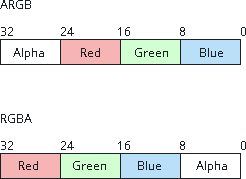
\includegraphics[width=20em]{imagens/sistema_rgba_argb.png}
	\caption{Sistema ARGB e RGBA, ambos com canais de 8 bits (1 byte)}
\end{figure}

Para realizar essa conversão basta aplicar um deslocamento de 24, 16 ou 8 bits conforme o canal e depois aplicar uma máscara de $0x0000FF_{16}$ bits (e.g $11111111_2$) para preservar somente o byte menos significativo. O tamanho do deslocamento depende da posição em que o canal se encontra. A extração do canal verde é exemplificada na figura a seguir.

\begin{figure}[H]
	\centering
	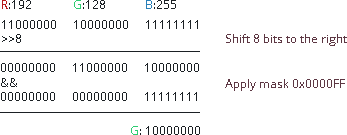
\includegraphics[width=22em]{imagens/extracting_rgb_channel.png}
	\caption{Extração do canal verde em um inteiro de 3 bytes}
\end{figure}

Uma vez que todos os dados foram inseridos no buffer, usa-se \texttt{buffer.flip()}. Antes de qualquer operação na textura vincula-se ela como atual usando \texttt{glBindTexture(type, id)}. Para este exemplo será utilizado o tipo \texttt{GL_TEXTURE_2D}, indicando uma imagem normal em 2D. Em seguida configura-se o modo de \textit{wrapping}. Por padrão, quando as coordenadas de uma textura excedem seu tamanho o openGL as repete com o modo \texttt{GL_REPEAT}. Entretanto, existem 4 modos possíveis: \texttt{GL_REPEAT}, \texttt{GL_MIRRORED_REPEAT}, \texttt{GL_CLAMP_TO_EDGE} e \texttt{GL_CLAMP_TO_BORDER}.
\begin{figure}[H]
	\centering
	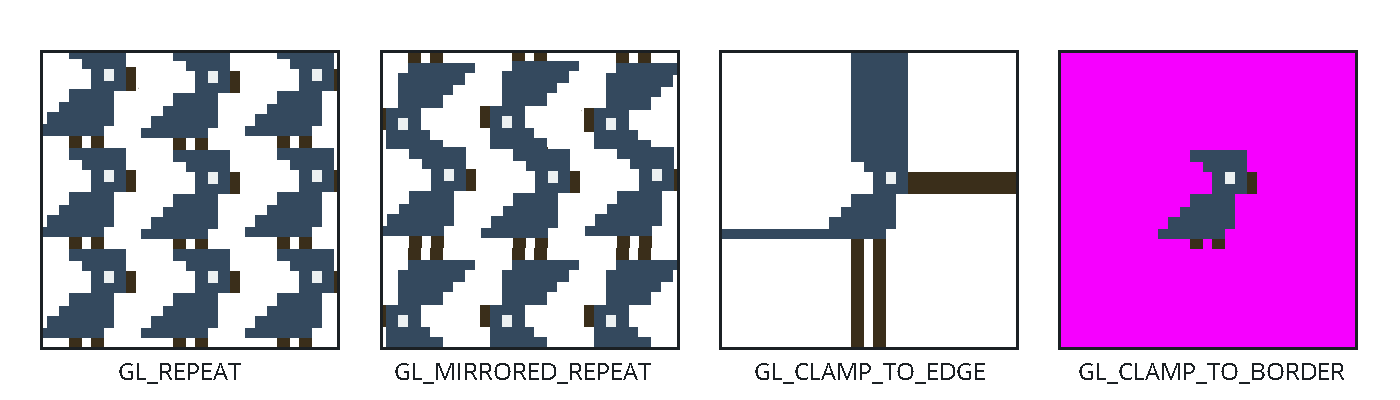
\includegraphics[width=\textwidth]{imagens/wrap_modes.png}
	\caption{Wrap modes}
\end{figure}
Esses modos são configurados através da função \texttt{glTexParameteri(GL_TEXTURE_2D, GL_TEXTURE_WRAP_S, GL_CLAMP_TO_EDGE)}. O segundo argumento indica o eixo para o qual se deseja aplicar a configuração, sendo eles S e T, equivalentes a x e y. Em seguida é escolhida a fórmula utilizada para escalonar a imagem. São dois modos possívei: \texttt{GL_NEAREST} e \texttt{GL_LINEAR}.

O modo \texttt{GL_NEAREST} é o modo \textit{default} do openGL e opera escolhendo o pixel cujo centro é o mais próximo da coordenada da textura. De uma maneira simples é o modo que ao ampliar a imagem não é aplicada nenhuma suavização, passando uma impressão de imagem serrilhada/pixelizada. A Figura~\ref{fig:ampli} demonstra esse processo.

O modo \texttt{GL_LINEAR} interpola um valor entre os pixels vizinhos. É o modo que ao ampliar ou diminuir a imagem causa uma impressão de bordas mais suaves.

\begin{figure}[H]
	\centering
	
\includegraphics[width=36em]{imagens/gl_filters.png}
	\caption{Ampliação de 32x usando cada tipo de filtro. \label{fig:ampli}}
\end{figure}

Esses modos podem ser aplicados distintamente para operações de aumentar ou diminuir a imagem. O atributo responsável por dizer em qual das duas situações o filtro deve ser aplicado é: \texttt{GL_TEXTURE_MAG_FILTER} e \texttt{GL_TEXTURE_MIN_FILTER}. Sendo o primeiro para operações de magnifying (aumento) e o segundo para operações de minifying (diminuir).

Por fim, com todos esses parâmetros configurados envia-se o bytebuffer contendo os dados da imagem propriamente dita para o OpenGL. Isso é feito na função \texttt{glTexImage2D(type, mipmap_level, internal_format, width, height, border, color_format, type, bytebuffer)}.

\subsection{Animações}
Uma vez que todo o sistema de shader program e texturas estão montados é possível usá-los para construir componentes mais avançados, como o de animação. Um objeto em animação não é nada mais que uma sequência de frames desenhados em um intervalo de milissegundos, criando ilusão de movimento. É comum a utilização de \textit{spritesheets} para armazenar todas as imagens em um único arquivo e então recortá-las em pedaços (frames) em tempo de execução.

\begin{figure}[H]
	\centering
	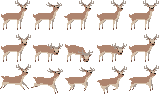
\includegraphics[width=16em]{imagens/spritesheet.png}
	\caption{Spritesheet com frames de 32x32 pixels}
\end{figure}
Para que esse recorte seja possível é necessário acrescentar alguns parâmetros ao shader para que este saiba qual pedaço deve ser recortado. Essa tarefa pode ser facilmente realizada alterando as coordenadas locais da textura enviadas através do atributo \texttt{glAttribXXXX} 0 definido anteriormente.


\begin{lstlisting}[caption=Vertex shader com animações]
#version 330 core
layout (location = 0) in vec4 vertex;
//Onde: xy coord. vertex e zw coord. textura
 
out vec2 TexCoords;
out vec3 FragPos;

uniform mat4 model;
uniform mat4 projection;
uniform mat4 camera;
uniform vec4 spriteFrame;
//Onde: xy coord. do frame na textura e zw largura e altura

void main(){
	vec2 tCoords = vertex.zw;

	tCoords *= spriteFrame.zw;
	tCoords += spriteFrame.xy;

	TexCoords = tCoords;
	gl_Position = projection * camera * model *  vec4(vertex.xy, 0.0 , 1.0);
	FragPos = vec3(model * vec4(vertex.xy , 0.0, 1.0));
}

\end{lstlisting}

Na variável \texttt{spriteFrame}  tem-se as coordenadas de qual pedaço da textura deverá ser extraído. Essa informação é então repassada  para o fragment shader onde por fim a função \texttt{texture()} irá colher esses pixels para manipulação.

Dessa forma o código da classe responsável pela manipulação lógica da animação fica como se segue. A classe pode ser ainda estendida para comportar frames com tempo de duração específico. Para isso basta substituir o parâmetro \texttt{long frameDuration} por um vetor com o tempo de duração correspondete a cada frame e alterar a lógica do método \texttt{update}.

\begin{lstlisting}[caption=Classe Animation]
public class Animation implements Serializable{
	private Vec4 frames[];
	private int currentFrame = 0;
	private String texture;
	private long frameDuration = -1;
	private long startTime = System.nanoTime();
	private boolean playedOnce = false;
	
	public Animation(String texture, long frameDuration) {
		this.texture = texture;
		this.frameDuration = frameDuration;
	}

	public void setFrames(int quantity, Vec2 offset, Vec2 size) {
	
		frames = new Vec4[quantity];
		float width = ResourceManager.getSelf().getTexture(texture).getWidth();
		float height = ResourceManager.getSelf().getTexture(texture).getHeight();
		
		for(int i= 0; i< quantity; i++){
			frames[i] = new Vec4(
						((float)i*size.x + offset.x)/width,
						(offset.y)/height,
						(size.x)/width,
						(size.y)/height
					);
		}
		
	}
	
	public Vec4 getCurrentFrame() {
		return frames[currentFrame];
	}
	
	public void update() {
		if(frameDuration>0) {
			long elapsed = (System.nanoTime() - startTime) / Engine.MILISECOND;
			
			if(elapsed > frameDuration) {
				currentFrame++;
				startTime = System.nanoTime();
			}
			if(currentFrame == frames.length) {
				currentFrame = 0;
				playedOnce = true;
			}
		}
	}
}
\end{lstlisting}
\subsection{Z-Ordering}
A técnica de z-ordering consiste na ordenação de objetos em sobreposição. É utilizada para organizar a ordem na qual os elementos devem ser renderizados tal que não haja elementos distantes sendo desenhados em cima de objetos mais próximos da câmera.
Para ambientes 2D, basta ordenar os elementos pela posição y do menor para o maior. 

\begin{figure}[H]
	\centering
	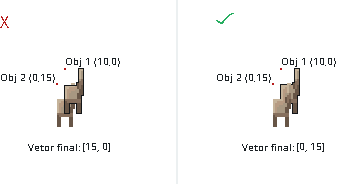
\includegraphics[width=28em]{imagens/z-order.png}
	\caption{Ordem correta de renderização: do menor y para o maior y}
\end{figure}

Deve atentar-se na implementação desta técnica para ordenar apenas os objetos que estão no espaço de visão da câmera, otimizando assim a performance do algoritmo de ordenação. É ainda necessário, para dar um melhor senso de profundidade, considerar a posição dos objetos a partir da sua base que toca o solo. Isto é, considerar que sua posição y no espaço seja relativa ao ponto no qual o objeto toca o chão invés de ser simplesmente o canto superior esquerdo da imagem. Esse mesmo principio de caixa base é utilizada para calcular a colisão dos objetos que caminham pelo ambiente.


\begin{figure}[H]
	\centering
	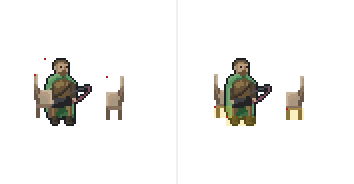
\includegraphics[width=28em]{imagens/zOrderWithBaseBox.png}
	\caption{Ordem correta de renderização: do menor y para o maior y considerando a caixa base}
\end{figure}



\section{Iluminação}
Existem muitos modelos de iluminação com equações sofisticadas que conseguem simular a luz de maneira muito próxima da realidade. Entretanto, estes modelos mais robustos não costumam servir para um sistema de tempo real pois são muito caros em perfomance, sendo geralmente utilizados em outras indústrias como, por exemplo, a cinematográfica.
O modelo de iluminação adotado e adaptado nesta engine foi o~\citeonline{phong1975} que usa três componentes de luz em sua construção: ambient, diffuse e specular~\cite{PhongShading}.

\begin{figure}[H]
	\centering
	
\includegraphics[width=28em]{imagens/lightning.png}
	\caption{Componentes do modelo de Phong}
\end{figure}




\subsection{Ambiente}
A luz ambiente representa as fontes de luz mais distantes que estão quase sempre presentes no mundo real como, por exemplo, o sol. São essas fontes que garantem a visibilidade quase constante dos objetos pois, afinal, sem luz o ser humano não é capaz de perceber o mundo visível.

Vale ressaltar duas propriedades importantes da luz: reflexão e refração. A iluminação que advém de qualquer fonte luminosa pode impactar objetos mesmo que estes não estejam sobre alcance direto. Esse efeito advém da propriedade da reflexão e é chamado de luz indireta. Algoritmos que levam esse fator em consideração são chamados de \textit{global illumination}, mas geralmente custam caro em performance ou são muito complexos.
Para esta engine será adotado um modelo simplificado que consiste em multiplicar a cor do objeto por uma variável \texttt{lightAmbientColor}, que define a cor e intensidade da luz que ilumina todo o mundo.

\begin{lstlisting}[caption=Fragment Shader com luz ambiente]
#version 330 core
in vec2 TexCoords;
out vec4 color;

uniform sampler2D image;

void main(){
	vec4 lightAmbientColor = vec4(1.1,0.7,0.25,1);
	
	vec4 imgTex =  texture(image, TexCoords).xyzw;
	
	color = imgTex*lightAmbientColor;
}
\end{lstlisting}

Dessa forma o resultado que se obtêm com a cor acima é um ambiente com uma tonalidade um pouco alaranjada:

\begin{figure}[H]
	\centering
	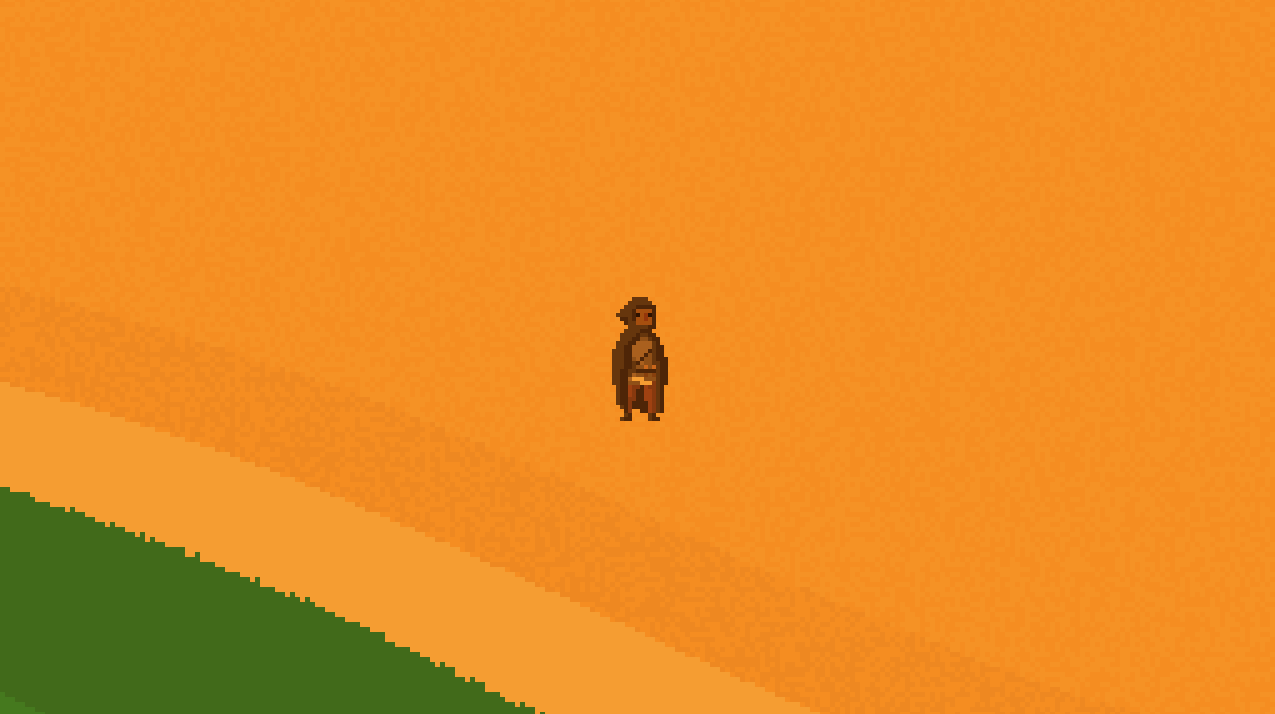
\includegraphics[width=28em]{imagens/sunset.png}
	\caption{Demonstração da luz ambiente com tonalidade alaranjada}
\end{figure}


\subsection{Luz Difusa}
A luz difusa simula o impacto direcional que uma fonte de luz tem sobre um objeto qualquer. Quanto mais perto o objeto está dessa fonte, mais iluminado ele será.

Para calcular a luz difusa é necessário antes ter em mãos o vetor normal do objeto que será atingido pelos raios de luz. Dessa forma, quando o raio de luz atinge o objeto calcula-se o ângulo de incidência $\theta$ entre os dois vetores usando o produto escalar. Note-se que o ângulo de reflexão é sempre igual ao ângulo de incidência.

\begin{figure}[H]
	\centering
	
\includegraphics[width=20em]{imagens/normal_reflection.png}
	\caption{Ângulo $\theta$ entre raio luminoso e vetor normal da superfície iluminada}
\end{figure}

O resultado desse produto escalar indica o impacto que a luz terá sobre a cor do fragmento sendo processado pelo shader, tendo em conta sua orientação relativa à luz. Para realizar o cálculo será necessário  então um vetor com a posição da fonte luminosa e o vetor normal do fragmento sendo afetado por essa fonte.
O vetor normal será obtido através de uma \textit{normal texture} e o vetor da fonte luminosa através de uma variável \texttt{global uniform}. O vetor normal é pré-calculado e armazenado em uma imagem enviada ao shader juntamente com as \textit{uniforms} posição e cor da fonte luminosa. O cálculo é então feito normalizando a subtração do \texttt{lightPos} pela posição do fragmento, obtendo assim o vetor direção da luz. Com o valor normalizado realiza-se o produto escalar da direção da luz pela normal contida na textura. Multiplica-se então o resultado pela cor da luz e ao final soma-se a luz difusa a luz ambiente. Esse resultado é multiplicado pela textura para obter o resultado final.

\begin{lstlisting}[caption=Fragment Shader com luz ambiente e difusa]
#version 330 core

in vec2 TexCoords;
in vec3 FragPos;  

out vec4 color;

uniform sampler2D image;
uniform sampler2D normalTex;

uniform vec3 lightPos; 
uniform vec3 lightColor;

void main(){

	vec3 normal = normalize(texture(normalTex, TexCoords).xyz);

	vec3 lightDir = normalize(lightPos - FragPos);
	float diff = max(dot(normal, lightDir), 0.0);
	vec3 diffuse = diff * lightColor;
	
	vec4 lightAmbientColor = vec4(1.1,0.7,0.25,1);
	vec4 imgTex =  texture(image, TexCoords).xyzw;
	
	color = imgTex * (lightAmbientColor + vec4(diffuse.xyz,1));
}
\end{lstlisting}



\begin{figure}[H]
	\centering
	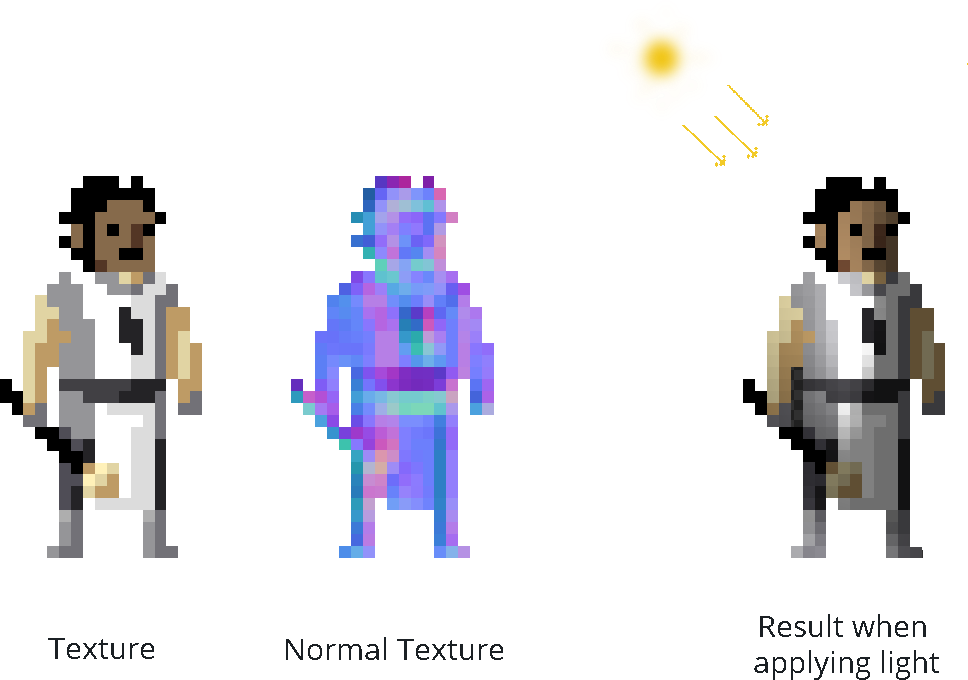
\includegraphics[width=20em]{imagens/normalTextureExample.png}
	\caption{Resultado da luz difusa usando a textura normal do objeto}
\end{figure}

\subsection{Vetor Normal}

Um vetor normal unitário é aquele perpendicular à superfície. A técnica habitualmente utilizada para trabalhar com vetores normais de um objeto consiste em mapeá-los para uma textura de forma que, para cada pixel da textura original, haja um vetor normal. Como o vetor normal precisa de apenas 3 coordenadas (x,y,z) isso é facilmente feito calculando-se a normal de cada pixel da textura e convertendo esse vetor para as coordenadas de cores RGB, que são por fim armazenadas em uma outra imagem chamada de textura normal.

\subsection{Luz Especular}
A luz especular é o ponto brilhante que aparece em objetos lisos e reluzentes, ajudando numa melhor percepção do espaço 3D e da textura do objeto que a reflete. A luz especular é mais intensa e presente numa superfície perfeitamente lisa de, por exemplo, um espelho. O brilho gerado por essa fonte luminosa é da cor da luz e não da cor do objeto.

Assim como a luz difusa, a luz especular possui o vetor de direção da luz e o vetor normal do objeto. Entretanto, ela também é calculada baseando-se na direção em que a câmera está olhando.


\begin{figure}[H]
	\centering
	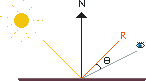
\includegraphics[width=20em]{imagens/specular.png}
	\caption{Luz especular do ponto de vista do observador}
\end{figure}

\subsection{Atenuação}
A intensidade da luz diminui quanto maior a distância de um objeto, começando intensa e rapidamente desvanecendo. Aplicar uma fórmula linear para calcular esse efeito daria uma impressão errônea do comportamento da luz, tratando-a como se fosse uniforme. Portanto, faz-se necessário utilizar uma fórmula que melhor simule este comportamento. Sendo ela:

\begin{center}
$F = \frac{1} {(K_c + K_l*d + K_q*d^2)}$
\end{center}

Aonde:
\begin{itemize}
    \item $K_c$ é uma constante arbitrária para garantir que o denominador nunca seja 0
     \item $K_l$ é uma constante linear
     \item $K_q$ é uma constante quadrática
     \item $d$ é a distância do fragmento até a fonte luminosa
\end{itemize}

Existe uma tabela para auxiliar na escolha do valor dessas constantes para distâncias entre 0 e 3200. A tabela \ref{tab:attenuationValues} pode ser facilmente estendida para distâncias maiores.


\begin{table}[H]
\centering

\begin{tabular}{l l l l}
Range & Constant & Linear & Quadratic \\
\hline		
3250 & 1.0 & 0.0014 & 0.000007 \\
600 & 1.0 & 0.007 & 0.0002 \\
325 & 1.0 & 0.014 & 0.0007 \\
200 & 1.0 & 0.022 & 0.0019 \\
160 & 1.0 & 0.027 & 0.0028 \\
100 & 1.0 & 0.045 & 0.0075 \\
65 & 1.0 & 0.07 & 0.017 \\
50 & 1.0 & 0.09 & 0.032 \\
32 & 1.0 & 0.14 & 0.07 \\
20 & 1.0 & 0.22 & 0.20 \\
13 & 1.0 & 0.35 & 0.44 \\
7 & 1.0 & 0.7 & 1.8  \\

\end{tabular}
\caption{Tabela de valores exemplo para a função de atenuação}
\label{tab:attenuationValues}
\end{table}

A implementação do fator de atenuação é feita diretamente no shader multiplicando os valores da luz ambiente, difusa e especular.

\begin{lstlisting}[caption={Fragment Shader com luz ambiente, difusa e atenuação}]
#version 330 core

in vec2 TexCoords;
in vec3 FragPos;  

out vec4 color;

uniform sampler2D image;
uniform sampler2D normalTex;

uniform vec3 lightPos; 
uniform vec3 lightColor;

void main(){

	vec3 normal = normalize(texture(normalTex, TexCoords).xyz);

	vec3 lightDir = normalize(lightPos - FragPos);
	float diff = max(dot(normal, lightDir), 0.0);
	vec3 diffuse = diff * lightColor;
	
	float distance = length(lightPos - vec3(FragPos.xyz));
	float constant = 1;
	float linear = 0.007;
	float quadratic = 0.0002;
	
	float attenuation = 1 / (constant + linear * distance + quadratic * (distance* distance));
	
	vec4 lightAmbientColor = vec4(1.1,0.7,0.25,1);
	vec4 imgTex =  texture(image, TexCoords).xyzw;
	
	color = vec4((imgTex.xyz + lightAmbientColor + (lightColor * attenuation*0.8) ) * attenuation, imgTex.w);
}
\end{lstlisting}

\section{Classe Renderer}
A classe renderer é responsável por conter e controlar todos métodos de desenho do sistema. Nela define-se uma função única tal que não seja necessário, a todo momento, configurar o shader e atualizar diretamente as variáveis uniform, VBO e VAO. Ela abstrai todos esses processos em uma simples chamada que recebe como argumento as coordenadas, textura e afins do objeto. Dessa forma, o código \ref{alg:initVBOVAO} será incorporado em uma classe renderer juntamente com o método render descrito a seguir. Note que é importante abstrair como parâmetros apenas aquilo necessário para a renderização, evitando passar objetos específicos do jogo em criação. Dessa maneira o sistema se mantém flexível o suficiente para desenvolvimento de jogos de qualquer tipo.


\begin{lstlisting}[caption=Classe renderer simples]
public class TextureRenderer(){

	public TextureRenderer(){
		init();
	}

	private void init(){
		//code from algorithm 4.7
	}

	public void render(Texture texture, Vec2 position, Vec2 size, float rotate, Vec4 color, Vec4 spriteFrame) {
		this.shader.use();
		Mat4 model = new Mat4();
		
		model = model.translate(position.x, position.y, 0);
		model = model.translate(0.5f * size.x, 0.5f *size.y, 0); //Move the origin of rotation to object's center
		model = model.rotate(rotate, 0, 0, 1); // Must be in radians
		model = model.translate(-0.5f * size.x, -0.5f *size.y, 0); //Move the origin of rotation back to it's top left
		model = model.scale(size.x, size.y, 1);
		
		shader.setMat4("model", model);
		shader.setVec4("spriteColor", color);
		shader.setVec2("flip", orientation);
		shader.setVec4("spriteFrame", spriteFrame);
		
		shader.setInteger("image", 0);
		
		glActiveTexture(GL_TEXTURE0);
		texture.bind();

		glBindVertexArray(quadVAO);
		glDrawArrays(GL_TRIANGLES, 0, 6*3);
		glBindVertexArray(0);
	}
}
\end{lstlisting}


Dessa forma, para renderizar os objetos itera-se numa lista e para cada objeto chama-se TextureRenderer.render().

\begin{lstlisting}[caption=Demonstração do render]
	for(GameObject obj: listOfObjects){
		textureRenderer.render(obj.getTexture(), obj.getPosition(), obj.getSize(), obj.size(), ...);
	}
\end{lstlisting}

Entretanto, esta implementação não é ideal pois faz-se necessário realizar n chamadas à função render, sendo n a quantidade de objetos na lista. Ou seja, se há um milhão de objetos na tela serão realizadas um milhão de chamadas ao método render e consequentemente um milhão de trocas de contexto de shader em this.shader.user() mais 4 transferências de informação para as variáveis uniform por chamada do método. Toda essa troca de contexto e transferência de dados entre CPU e GPU possuem um impacto enorme no desempenho. E quanto maior a lista de objetos a serem desenhados pior será a performance.

Para fins de introdução ao conceito e simplificação do processo de renderização abordou-se o modelo acima. Entretanto, o problema será tratado em uma sessão mais adiante que implementará o método de \textit{batch rendering}, resolvendo esta situação realizando uma única chamada do método render por tipo de shader e texture. Dessa forma, a transferência dos dados será feita em um único e enorme pacote, evitando gargalo no BUS da placa mãe e \textit{overhead} de funções.

\section{Arquitetura do Game Object}

Os \textit{game objects}, também conhecidos como entidades, estão no centro de tudo aquilo que dá vida ao cenário do jogo. São esses arquétipos que definem NPC's, inimigos, vida selvagem e até mesmo o próprio jogador. Existem três arquiteturas muito presentes e comuns no desenvolvimento de games: \textit{Component Based}, \textit{Object Oriented} e \textit{Entity System} \cite{GameObjectArchitecture}. 

\subsection{Object Based}
Uma arquitetura baseada em objetos trabalha sobre o conceito de hierarquia de classes. Haverá uma classe \texttt{GameObject} que é então especializada para cada tipo de objeto. Por exemplo, uma classe \texttt{Minotauro} estende uma classe \texttt{Monstro} que, por sua vez, estende a classe \texttt{GameObject}. Da mesma forma uma classe \texttt{Besouro} estende a classe \texttt{Monstro} que estende a classe \texttt{GameObject}.

O problema dessa implementação é que quanto mais especializações são criadas mais difícil e complexo se torna a manutenção dessa estrutura. Para cada nova regra implementada em uma especialização surgem exceções que começam a tornar necessário uma generalização ainda maior, resultando em uma classe \texttt{GameObject} extensa e com recursos muitas vezes usados apenas por uma única especialização.

Isso ainda pode causar relações de hierarquia que não fazem sentido lógico como, por exemplo, uma armadilha que estende a classe \texttt{Monstro} só para ser capaz de usar o sistema de dano.


\begin{figure}[H]
	\centering
	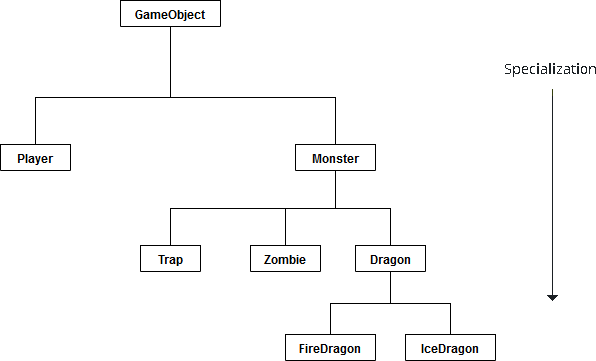
\includegraphics[width=26em]{imagens/gameobject_specialization.png}
	\caption{Especialização das classes numa arquitetura baseada em objetos}
\end{figure}

\subsection{Component Based}
A arquitetura baseada em componentes, também conhecida pelo nome de \textit{behavior}, consiste no uso de composição invés de herança. Ao contrário da especialização e generalização utilizados na herança o sistema de composição consiste em criar vários pequenos componentes e então ``especializar'' um \texttt{GameObject} atribuindo a ele os componentes que se deseja. Dessa forma, para que um \texttt{GameObject} seja um \texttt{Monstro} basta adicionar um componente de dano, vida e IA, por exemplo.

Dessa forma, quando o sistema for salvar o \textit{game object} não será desperdiçada memória salvando dados de outros sistemas que não estão sendo utilizados por esse objeto pois, da maneira agora proposta, cada \textit{game object} terá apenas os componentes de que necessita e fará uso.

Existem várias maneiras de se implementar essa arquitetura. Através do uso de \textit{switches} para assinalar qual componente está ativo ou não, através do padrão de projeto com componentes passando mensagem entre outros. A maior desvantagem dessa arquitetura está na relação acoplada entre  dados e o sistema que os manipula.

\begin{figure}[H]
	\centering
	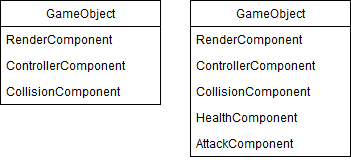
\includegraphics[width=20em]{imagens/componentBased.png}
	\caption{GameObject composto de vários componentes}
\end{figure}


\subsection{Entity Based}
Um game object baseado em entidades trabalha de maneira similar à forma como um banco de dados trata suas informações. O sistema que manipula as informações é desacoplado dos dados em si. Dessa maneira, uma entidade é composta apenas de dados e um sistema à parte é responsável por processar essas informações e realizar suas tarefas.
Assim, uma entidade do tipo \texttt{Monstro} precisa ter associado a ela apenas os atributos pertinentes como dano, vida e IA. O sistema então responsável verifica se a entidade possui esses atributos e, caso tenha, realiza seus cálculos senão, o sistema ignora essa entidade e avança para a próxima da lista.

//TODO: citar a figura indicando que os componentes foram desenvolvidos.


\begin{figure}[H]
	\centering
	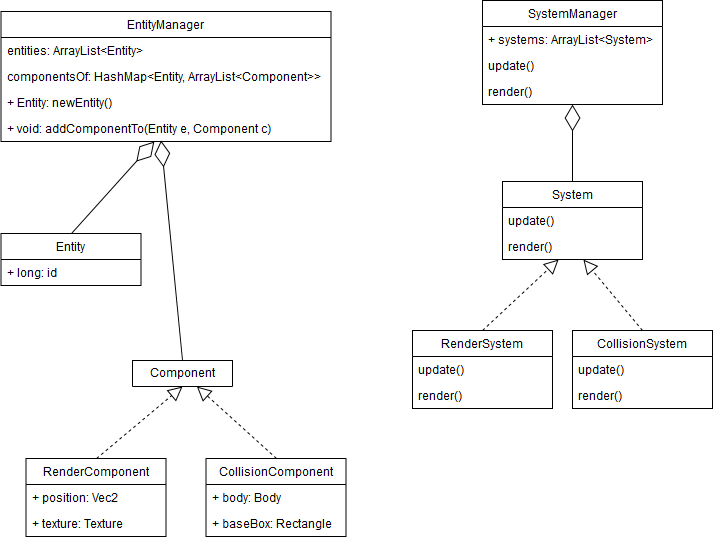
\includegraphics[width=30em]{imagens/entityDiagram.png}
	\caption{Diagrama de classes do sistema entity based}
\end{figure}

//TODO: cód.

\section{Sistema de colisões}

O sistema de colisões é responsável por delimitar o espaço físico que cada objeto deve ocupar no ambiente. Para formas geométricas mais básicas como retângulos, círculos e triângulos existem fórmulas simples e otimizadas para detectar essas colisões. Para polígonos mais complexos existem diversos algoritmos que usufruem de métodos avançados para detectar e resolver essas colisões.

Um problema de colisão é dividido em duas etapas: detecção e resolução. A etapa de detecção consiste em detectar quais objetos colidiram com quais outros objetos em um tempo $t$. Esse processo pode ocorrer de duas formas, por antecipação ou no tempo de colisão. A segunda etapa consiste em resolver essas colisões usando uma série de critérios como, por exemplo: gravidade, massa, velocidade, impulso, torque entre outros.

\subsection{Colisões do tipo AABB vs AABB}

Colisões do tipo Axis Aligned Bounding Box (AABB) são as mais simples de resolver. Um retângulo do tipo AABB possui o seu eixo $x$ paralelo ao eixo x do plano cartesiano, e o seu eixo y paralelo ao eixo y do plano cartesiano, ou seja, sem qualquer rotação. Para detectar se dois retângulos de eixo alinhado colidiram basta checar se houve sobreposição em qualquer um dos eixos x e y.

\begin{lstlisting}[caption=Colisão AABB vs AABB]
	public boolean intersects(Rectangle r) {
    	float tw = this.width;
        float th = this.height;
        float rw = r.width;
        float rh = r.height;
        
        if (rw <= 0 || rh <= 0 || tw <= 0 || th <= 0) 
            return false;
        
        float tx = this.x;
        float ty = this.y;
        float rx = r.x;
        float ry = r.y;
        rw += rx;
        rh += ry;
        tw += tx;
        th += ty;
      
        return ((rw < rx || rw > tx) && 
                (rh < ry || rh > ty) &&
                (tw < tx || tw > rx) && 
                (th < ty || th > ry)); 
    }
\end{lstlisting}


\begin{figure}[H]
	\centering
	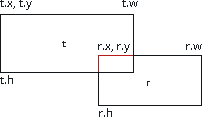
\includegraphics[width=16em]{imagens/aabbaabb.png}
	\caption{Colisão AABB vs AABB}
\end{figure}

Para o exemplo da figura acima a intersecção ocorreu onde $rw > tx$, $rh > ty$, $tw > rx$ e $th > ry$. Ou seja, o retângulo r está abaixo e a direita do retângulo t.

\subsection{jBox2D}

A biblioteca jBox2D é um porte da biblioteca Box2D, originalmente implementada em C++. Trata-se de uma ferramente rica em recursos para manipulação de corpos rígidos 2D. Embora o sistema de medidas implementado pelo jBox2D esteja no padrão internacional (metros) isso não o torna inutilizável para um ambiente 2D com sistema de medida em pixels. Entretanto, faz-se necessário criar um fator de escala para converter entre um sistema e outro. Para o sistema de colisões funcionar ele precisa, assim como a própria engine, de um mundo e um timestep, neste caso, fixo. Esse sistema será então atualizado juntamente com o método \texttt{update()} da engine.

//TODO: cód.

\section{Sistema de coordenadas}

O sistema de coordenadas compreende todo o processo de manipulação das coordenadas de um game object para a tela final do usuário. Esse processamento tem início em espaço local e termina na sua conversão final para \textit{Normalized Devide Coordinates} (NDC) que por fim é rasterizado pelo OpenGL na tela. Note que o OpenGL espera todas as coordenadas finais no formato NDC, que varia entre $[-1,1]$. São cinco sistemas de coordenadas:

\begin{enumerate}
    \item Espaço local
    \item Espaço de mundo
    \item Espaço de visão (ou espaço de câmera)
    \item Espaço de recorte
    \item Espaço da tela
\end{enumerate}

Uma vez processadas elas são passadas para o \textit{shader rasterization} e enfim convertidas para pixels 2D na tela.

\begin{figure}[H]
	\centering
	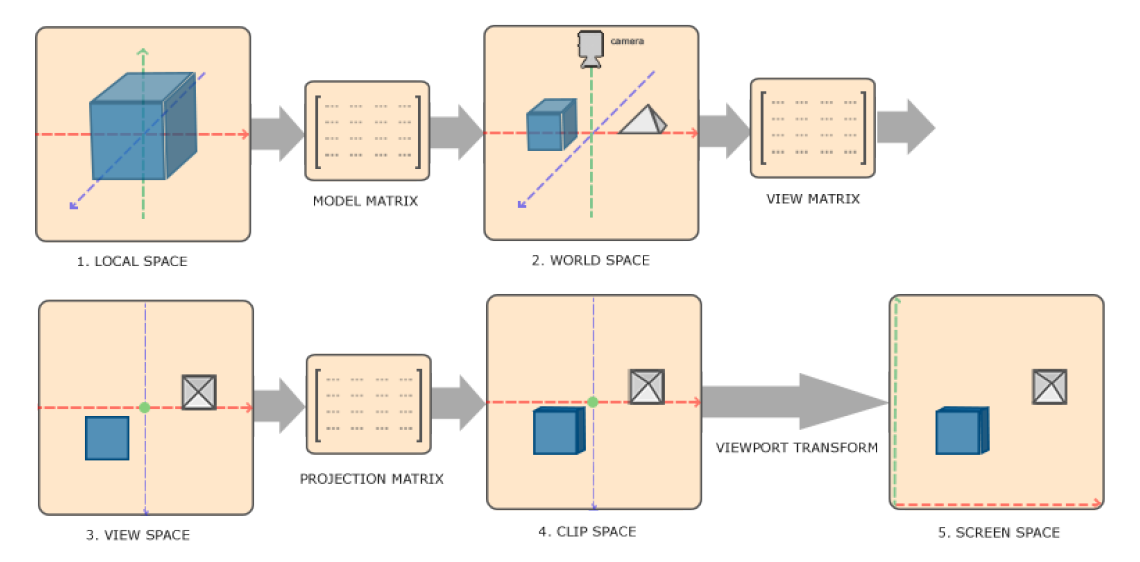
\includegraphics[width=30em]{imagens/coordSpace.png}
	\caption{Processo de transformações de coordenadas até o espaço final da tela. Fonte:~\cite{LearnOpenGL}}
\end{figure}

\subsection{Espaço local}
As coordenadas em espaço local referem-se ao próprio espaço do objeto. Representam as coordenadas do objeto relativo à sua própria origem. Geralmente são normalizadas no formato NDC com origem no ponto $(0,0)$.


\subsection{Espaço de mundo}
As coordenadas em espaço de mundo são obtidas através da multiplicação do espaço local pela matriz \textit{model}. O resultado representa a posição do objeto no mundo relativo à origem do mundo. O processo de multiplicação do espaço local pela matriz \textit{model} escala, rotaciona e translada o objeto para o espaço de mundo através do processo chamado transformação afim \cite{AffineTransformation}.

\begin{figure}[H]
	\centering
	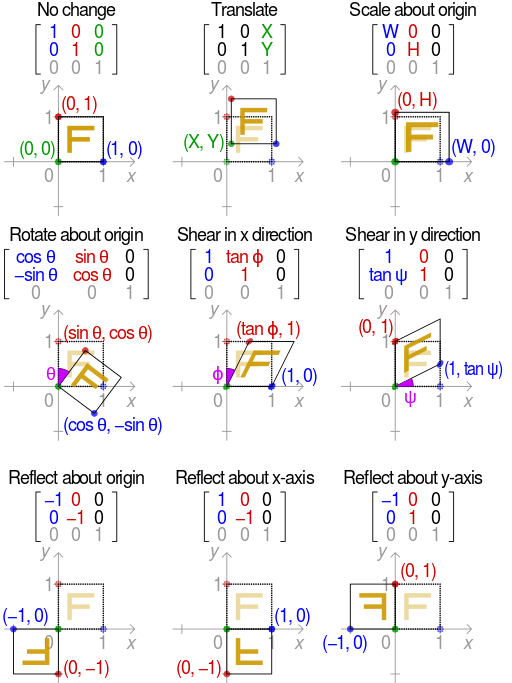
\includegraphics[width=20em]{imagens/affineTransformation.png}
	\caption{Exemplos de transformação afim. Fonte:~\cite{AffineTransformationImg}}
\end{figure}

Se todos os objetos fossem inseridos no mundo somente usando as coordenadas locais muito provavelmente estariam sobrepostos na origem. O processo de conversão para o espaço de mundo pode ser exemplificado por uma pilha de caixas onde se deseja inserir outra. Para empilhá-la é necessário escalá-la para o mesmo tamanho das outras, rotacioná-la para alinhar e, por fim, transladá-la para a posição na pilha.

\subsection{Espaço de visão}
O espaço de visão, também referenciado como espaço da câmera, é obtido a partir da multiplicação do espaço de mundo pela \textit{view matrix} e representa o ponto de vista da câmera sobre o mundo.

\subsection{Espaço de recorte}
Espaço de recorte é a zona visível na tela de forma que todos os pontos fora desse espaço são descartados. Para que o usuário não tenha de especificar todas coordenadas em um intervalo NDC desde o início do processo trabalha-se com dois sistemas de projeção responsáveis por converter do espaço de visão de volta para um intervalo NDC. São os dois sistemas: projeção ortográfica e projeção de perspectiva.
Note que, se um triângulo possui apenas um parte visível e terá uma parte recortada o OpenGL divide esse triângulo em primitivas menores e então descarta aquelas que estão fora da tela.

\subsection{Projeção}

Existem duas formas de projeção, ambas baseadas no conceito de frustum, porção de um sólido contido entre duas bases paralelas que o cortam \cite{Frustum}. Os dois tipos de projeção são: ortográfica e perspectiva. A primeira é composta de um frustum retangular e a segunda de um frustum com formato similar a uma pirâmide.

\subsubsection{Projeção ortográfica}

Para especificar uma matriz de projeção ortográfica é necessário fornecer a largura, altura e comprimento do frustum. Dessa forma, todas as coordenadas que estiverem entre o plano mais próximo e o plano mais distante serão preservadas e desenhadas na tela. Todo o resto será recortado fora.

\begin{figure}[H]
	\centering
	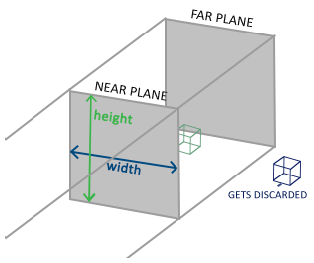
\includegraphics[width=20em]{imagens/orthographicProjection.png}
	\caption{Frustum da projeção ortográfica. Fonte:~\cite{LearnOpenGL}}
\end{figure}

A projeção ortográfica mapeia linearmente coordenadas 3D diretamente para o plano 2D da tela, sem levar em consideração a perspectiva. Isso produz um efeito não realístico para ambientes 3D pois passa a impressão de objetos prensados na tela, sem profundidade.

Para especificar a matriz ortográfica será utilizada a função do GLM definida a seguir. Os dois primeiros parâmetros são as coordenadas esquerda e direita do frustum, o terceiro e quarto parâmetro a parte de baixo e topo do frustum. Com esses quatro parâmetros definiu-se o tamanho do plano mais próximo e do plano mais distante. O quinto e sexto parâmetro indicam a distância entre os dois planos.

\begin{lstlisting}[caption=Função Ortho do GLM]
Mat4 projection = new Mat4();
projection = projection.ortho(float left, float right, float bottom, float top, float zNear, float zFar);
\end{lstlisting}

\subsubsection{Projeção de perspectiva}
A projeção de perspectiva simula a percepção humana de profundidade. Objetos mais distantes se tornam menores e a esse efeito é dado o nome de perspectiva. Esse fenômeno acontece por que o ser humano enxerga o mundo a partir de dois olhos, com ângulos de visão distintos.

O frustum utilizado na projeção de perspectiva possui um formato similar a de uma pirâmide justamente para auxiliar na reprodução esse fenômeno. Ao invés de realizar uma transformação linear das coordenadas 3D para a tela, é feito um mapeamento que leva em consideração a distância dos objetos.

\begin{figure}[H]
	\centering
	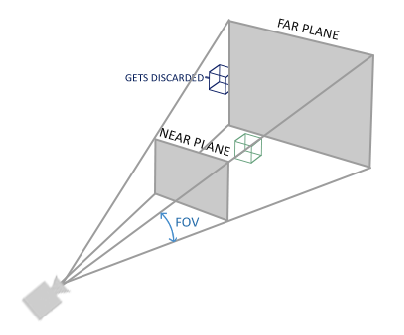
\includegraphics[width=20em]{imagens/perspectiveProjection.png}
	\caption{Frustum da projeção de perspectiva. Fonte:~\cite{LearnOpenGL}}
\end{figure}

A matriz de projeção pode ser criada utilizando a seguinte função do GLM onde o primeiro parâmetro recebe o field of view (FOV) em radianos, o segundo recebe a proporção de tela e no terceiro e quarto parâmetro recebe o plano mais próximo e distante, respectivamente.

\begin{lstlisting}[caption=Função Perspective do GLM]
Mat4 perspective = new Mat4();
perspective = perspective.perspective(toRadians(45), width/height, near, far);
\end{lstlisting}

\subsection{jBox2D para espaço de mundo}

Para trabalhar com os dois sistemas de medida (pixels e metros) basta selecionar um fator de escalonamento. Supondo um fator de 100, basta multiplicar por 100 para converter de metros para pixels e dividir por 100 para converter de pixels para metros.

\section{Câmera}
A classe câmera é responsável por manter, calcular e enviar o valor da matriz de visão para o uniform no shader. Ela é necessária pois, a partir de uma única classe fica fácil manipular em quem está o foco da câmera, aplicar efeitos como tremulação entre outras funções. É importante frisar que ela deve atualizar a variável uniform dentro do método \texttt{variableUpdate} para que seja utilizado o valor baseado na interpolação, caso contrário ela dará impressão de objetos travando como discutido na subseção de interpolação linear \ref{subsec:interpoLinear}.

\begin{lstlisting}[caption=Mouse input]
public class Camera {
    private float x=0,y=0,z=0;
    private Entity focus;
    private Mat4 camera;
    private Mat4 transform;
    private EntityManager em;
     
    public Camera(EntityManager em) {
        this.em = em;
        camera = new Mat4();
        transform  = new Mat4();
        camera = camera.identity();
    }
     
    public void setFocusOn(Entity entity) {
        focus = entity;
    }
     
    public void moveDirectTo(float x, float y) {
        this.x = x;
        this.y = y;
        camera = camera.identity();
        camera.translate(x, y,0);
    }
     
    public void move(float x, float y) {
        this.x += x;
        this.y += y;
        camera = camera.identity();
        camera.translate(this.x, this.y,0);
    }
     
    public void update(float deltaTime) {}
     
    public void variableUpdate(float alpha) {
        RenderComponent rc = ((RenderComponent)(em.getFirstComponent(focus, RenderComponent.class)));
        Vec2 position = rc.getRenderPosition();
        Vec2 size = rc.getSize();
         
        if(focus != null)
            moveDirectTo(-position.x + 1280/2 - size.x/2, -position.y +720/2 - size.y/2);
 
        transform = transform.identity();
        transform.translate(this.x,this.y,0);
         
        ResourceManager.getSelf().getShader("texture").use();
        ResourceManager.getSelf().getShader("texture").setMat4("camera", transform);
         
        ResourceManager.getSelf().getShader("batchRenderer").use();
        ResourceManager.getSelf().getShader("batchRenderer").setMat4("camera", transform);
    }
 
    public float getX() {
        return x*-1;
    }
 
    public float getY() {
        return y*-1;
    }
     
    public Vec2 getPos() {
        return new Vec2(x*-1,y*-1);
    }
}
\end{lstlisting}

\section{Sistema de input}
O sistema de input é responsável por mapear botões de uma interface física como teclado, mouse e controle de videogame em ações dentro do jogo. Para não lidar diretamente com a interface de hardware a biblioteca GLFW apresenta uma abstração que realiza essa comunicação.

O conceito para implementar o mapeamento de input consiste em definir um mapa de ações que podem então ser associadas ao input do usuário. Dessa forma, se o usuário trocar o equipamento, suponha-se, de um teclado para um controle de videogame tudo que o sistema precisa fazer é associar os novos botões às ações. Por exemplo, a ação de pular no teclado é mapeada para a tecla espaço. Quando o usuário trocar para o controle de videogame o sistema mapeia a ação pular para o botão "X" do controle, por exemplo. Dessa forma abstrai-se a ação que o game object vai realizar do hardware que está sendo utilizado.

Entretanto, haverá casos que essa abstração não será suficiente e as ações serão mapeadas diretamente ao hardware em uso. Essa situação irá ocorrer, por exemplo, na interação com a interface onde o cursor do mouse não é diretamente mapeável para o joystick. Seria necessário implementar um pseudo cursor usando os botões analógicos do controle ou mapear o movimento de tecla em tecla ao invés de usar o conceito de ponteiro.

\subsection{GLFW Keyboard}
Para o controle do teclado é necessário primeiro definir uma classe que irá implementar o callback do GLFW. Nela será criado um vetor de booleanos que indica quais teclas estão pressionadas em determinado momento.

\begin{lstlisting}[caption=Keyboard input]
public class KeyboardControl extends GLFWKeyCallback implements  Control {
    private boolean keys[] = new boolean[512];
 
    @Override
    public void invoke(long window, int key, int scancode, int action, int mods) {
        keys[key] = action != GLFW.GLFW_RELEASE;
    }
 
    @Override
    public boolean isKeyPressed(int key) {
        return keys[key];
    }
 
    @Override
    public boolean isKeyReleased(int key) {
        return keys[key];
    }
}
\end{lstlisting}

A partir da classe KeyBoardControl é possível implementar então um HashMap que mapeia as teclas para ações que serão então utilizadas pelos game objects.


\subsection{GLFW Mouse}
De maneira similar o controle do mouse contém um vetor de booleanos indicando quais teclas estão sendo pressionadas e também um Vetor de duas coordenadas indicando sua posição na janela. Note-se que as coordenadas são calculadas considerando o canto superior esquerdo da janela como origem.

\begin{lstlisting}[caption=Mouse input]
public class MouseControl extends GLFWCursorPosCallback implements Control{
    private int previousState = -1;
    private Vec2 cursorPos = new Vec2(0,0);
     
    @Override
    public boolean isKeyReleased(int key) {
        int state = glfwGetMouseButton(Engine.getSelf().getWindow().getId(), key);
         
        if (state == GLFW_RELEASE) 
            return true;
        else
            return false;
    }
 
    @Override
    public boolean isKeyPressed(int key) {
        int state = glfwGetMouseButton(Engine.getSelf().getWindow().getId(), key);
         
        if (state == GLFW_RELEASE &&  previousState== GLFW_PRESS) {
            previousState=state;
            return true;
        }else {
            previousState=state;
            return false;
        }
    }
 
    @Override
    public void invoke(long window, double xpos, double ypos) {
        cursorPos.x = (float) xpos;
        cursorPos.y = (float) ypos;
    }
 
    public Vec2 getCursorPos() {
        return cursorPos;
    }
}
\end{lstlisting}


\section{Gerência de recursos}
O sistema de gerência de recursos é responsável por ler e salvar todos os arquivos da engine. Em suma, esse sistema centraliza todas as operações de I/O num único lugar de forma que seja evitado a ocorrência de dois arquivos idênticos em memória. Isso é possível através do mapeamento dos recursos em um único lugar.


\subsection{Chunk}
Um chunk (em português, pedaço) contem todas as entidades que intersectam sua \textit{bounding box} e informações pertinentes do terreno como: textura, regiões de interação entre outros. Ele é serializado para leitura e escrita em disco. Sendo assim, um conjunto de $n$ chunks sendo carregados no início do jogo representam o último estado do jogo. Esse estado contém todas as entidades, mapa e outros artefatos  .

A geração da textura do mapa pode ser dinâmica, isto é, ser gerada a cada frame, ou estática, gerando-se uma única vez. A estática é utilizada para terrenos sem animação, enquanto a dinâmica para terrenos que envolvem animação como, por exemplo, as ondas que atingem a praia.

\subsection{Chunk system}
O sistema de chunks reparte toda a extensão do mapa em pequenos pedaços para uma maior facilidade de manuseio na hora de ler e salvar no disco. Um fator determinante para a escolha deste formato é a necessidade de poder gerar um mapa procedural e com carregamento dinâmico, ou seja, sem telas de carregamento. Isso é possível repartindo o mapa em pequenos pedaços que serão gerados, lidos e escritos sobre demanda.

É importante notar que este sistema é crítico e deve ser meticulosamente ajustado para as necessidades de cada projeto. Um arquivo muito grande pode gerar um atraso de leitura e escrita muito alto, enquanto um arquivo muito pequeno pode sobrecarregar o sistema com o \textit{overhead} de muitas chamadas de função I/O num período curto de tempo. É necessário implementar este sistema utilizando técnicas de leitura e escrita assíncronas de forma que a engine não congele enquanto aguarda operações de I/O.

Para tanto, o gerenciador de chunks armazena uma matriz 3 por 3 de chunks. Sempre que a câmera intersectar um chunk da borda será carregado uma nova coluna ou linha dessa matriz contendo os novos chunks que, caso ausentes no disco são gerados e, caso presentes, lidos. Esse processo deve ocorrer de forma rápida tal que o usuário não note qualquer chunk sendo carregado. Se o usuário movimentar-se mais rápido do que o sistema é capaz de carregar os chunks ele irá perceber várias partes cinzas que subitamente serão preenchidas com textura quando sua leitura finalizar.

\begin{figure}[H]
	\centering
	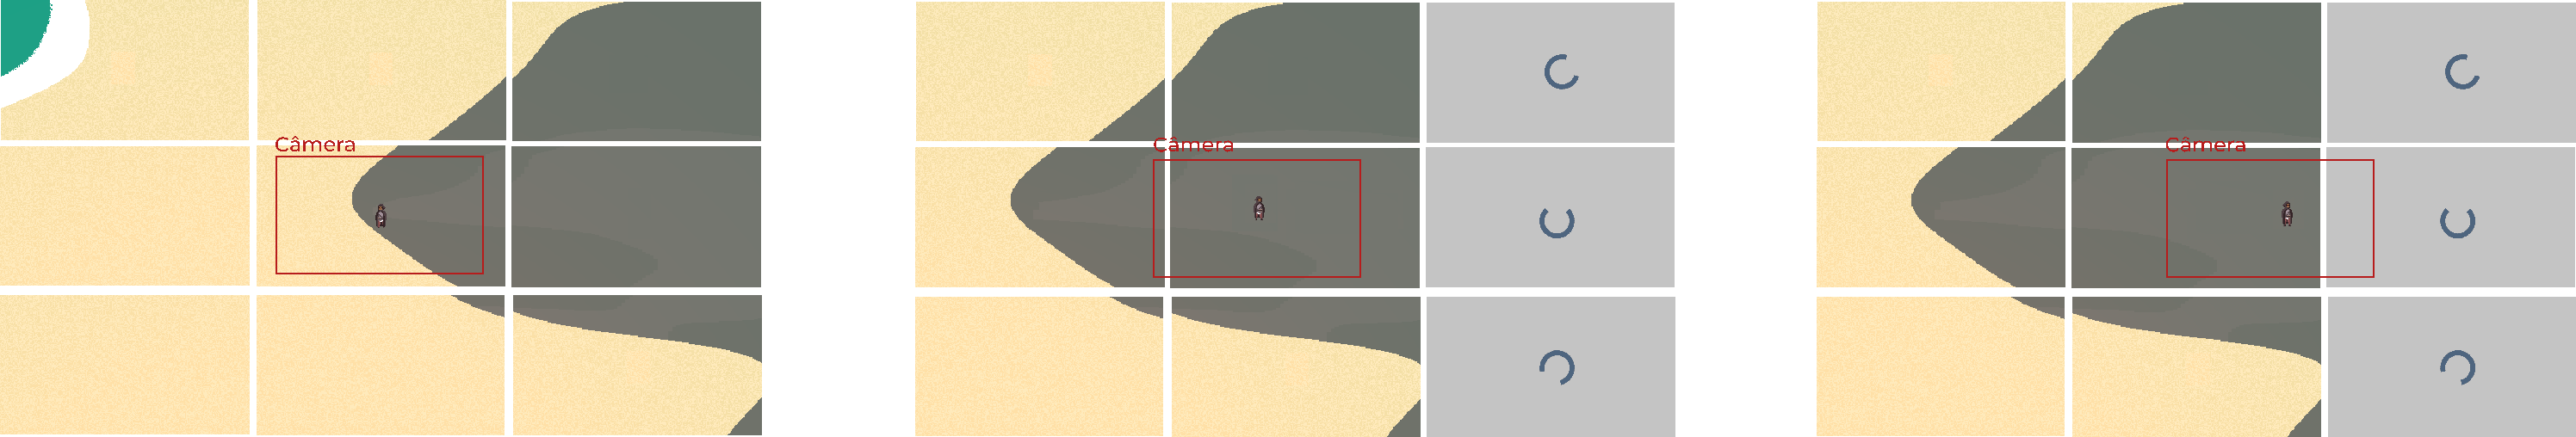
\includegraphics[width=38em]{imagens/chunkSystem.png}
	\caption{Demonstração do sistema de chunks carregando a última coluna da matriz}
	\label{fig:chunkSystem}
\end{figure}

O retângulo vermelho da figura \ref{fig:chunkSystem} representa a câmera. No momento em que esse retângulo intersecta qualquer um dos chunks na borda é iniciado o carregamento da linha e/ou coluna adjacentes a esse chunk. No caso da figura exemplo, quando a câmera intersecta o chunk da borda direita a primeira coluna da matriz é removida e armazenada em uma tabela Hash, enquanto a nova coluna direita da matriz é carregada. Se a câmera mover-se mais rápido do que o sistema é capaz de carregar os chunks o usuário irá presenciar partes cinzas na tela, que são as texturas ainda em carregamento.

\subsection{Chunk Manager}
O Chunk manager fica responsável por gerenciar quais chunks devem ser gerados, lidos ou salvos. Ele contém uma tabela hash com todos os chunks lidos até o momento, para evitar que tenham de ser lidos do disco caso já tenham sido em algum momento anterior.
Esse gerenciador também é responsável por controlar o processo de leitura assíncrona, retornando o elemento somente quando sua leitura ou escrita foi completada.

\subsection{A classe Resource Manager}
A classe responsável pela leitura e escrita desses arquivos segue o padrão de projeto Singleton, sendo assim facilmente invocada de qualquer lugar do código.

\begin{lstlisting}[caption=Classe Resource Manager]
 
public final class ResourceManager {
    private static ResourceManager self;
    private static HashMap<String,  Shader> shaders = new HashMap<String, Shader>();
    private static HashMap<String,  Texture> textures = new HashMap<String, Texture>();
    private static HashMap<String,  Audio> audio = new HashMap<String, Audio>();
    private static HashMap<String,  Font> fonts = new HashMap<String, Font>();
    private static HashMap<String,  Renderer> renderers = new HashMap<String, Renderer>();

    private ResourceManager() {}
     
    public static ResourceManager getSelf() {
        if(self == null) 
            self = new ResourceManager();
        return self;
    }
     
    public Audio loadAudio(String name, String audioPath) {
        if(audio.containsKey(name))
            return audio.get(name);
        return audio.put(name, new Audio(audioPath));
    }
     
    public Audio getAudio(String name) {
        return audio.get(name);
    }
     
    public Font loadFont(String name, String fontPath) {
        if(fonts.containsKey(name))
            return fonts.get(name);
        return fonts.put(name, new Font());
    }
     
    public Font getFont(String name) {
        return fonts.get(name);
    }
     
    public int playAudio(String name, Vec2 pos, float maxDistance) {
        AudioSource a = new AudioSource(audio.get(name).getBufferPointer(), pos, maxDistance);
        a.play();
         
        return a.getSourcePointer();
    }

    public Shader loadShader(String name, String vertexShaderPath, String fragmentShaderFilPath, String geometryShaderPath) {
        if(shaders.containsKey(name))
            return shaders.get(name);
        return shaders.put(name, loadShaderFromFile(vertexShaderPath, fragmentShaderFilPath, geometryShaderPath));
    }

    public Texture loadTexture(String name, String imgPath) {
        if(textures.containsKey(name))
            return textures.get(name);
        return textures.put(name, loadTextureFromFile(imgPath));
    }
     
    public Shader getShader(String name) {
        return shaders.get(name);
    }
     
    public Texture getTexture(String name) {
        return textures.get(name);
    }

    private Shader loadShaderFromFile(String vertexShaderPath, String fragmentShaderPath, String geometryShaderPath) {
        String vertexCode = null, fragmentCode = null, geometryCode = null;
         
        try {
            //Vertex Code
            StringBuilder stringBuilder = new StringBuilder();
            BufferedReader bufferedReader;
             
             
             
            bufferedReader = new BufferedReader(new InputStreamReader(
                    this.getClass().getResourceAsStream("/" + vertexShaderPath)
                    )); 
            String line;
             
            while((line = bufferedReader.readLine())!=null)
                stringBuilder.append(line).append("\n");
             
            bufferedReader.close();
            vertexCode = stringBuilder.toString();
             
            //Fragment Code
            stringBuilder = new StringBuilder();
             
            bufferedReader = new BufferedReader(new InputStreamReader(
                    this.getClass().getResourceAsStream("/" + fragmentShaderPath)
                    )); 
             
            while((line = bufferedReader.readLine())!=null)
                stringBuilder.append(line).append("\n");
             
            bufferedReader.close();
            fragmentCode = stringBuilder.toString();
             
            //Geometry Code
            if(geometryShaderPath!=null){
                stringBuilder = new StringBuilder();
                bufferedReader = new BufferedReader(new InputStreamReader(
                        this.getClass().getResourceAsStream("/" + geometryShaderPath)
                        )); 
                 
                while((line = bufferedReader.readLine())!=null)
                    stringBuilder.append(line).append("\n");
                 
                bufferedReader.close();
                geometryCode = stringBuilder.toString();
            }
        } catch (IOException e) {
            e.printStackTrace();
        }
         
        Shader shader = new Shader();
        shader.compile(vertexCode, fragmentCode, (geometryCode==null)? null : geometryCode);
        return shader;
    }
     
    private Texture loadTextureFromFile(String imgPath) {
        Texture t = new Texture("/"+imgPath); 
        return t;
    }
     
    public void setRenderer(String name, Renderer r) {
        renderers.put(name, r);
    }
     
    public <T extends Renderer> T getRenderer(String name) {
        return (T) renderers.get(name);
    }
}
\end{lstlisting}

\section{Aúdio}
A implementação de aúdio foi feita utilizando outra biblioteca multiplataforma da Khronos, o OpenAL, voltada especificamente para áudio. Através dela é possível utilizar diversas funções para manipulação de aúdio 3D numa maneira eficiente e ágil. 

\subsection{Integrando o OpenAL}
O openAL usa conceitos similares aos que são empregados no OpenGL. Cria-se e vincula-se buffers para transferir e receber dados através da API.
Sempre existe um único ouvinte por \textit{audio context}, que representa a posição de onde todas as fontes serão escutadas. Para definir uma fonte de aúdio é necessário primeiro carregar o aúdio do arquivo. O OpenAL por padrão usa buffers com formato Modulação por Código de Pulso(PCM) em 8 ou 16 bits, mono ou stereo.

Para ler o arquivo e prepará-lo para inserção no buffer é necessário carregá-lo usando a biblioteca auxiliar STBVorbis, que acompanha o LWJGL.
Lê-se o arquivo usando \texttt{this.getClass().getResourceAsStream}, em sequência aloca-se dois buffers de inteiro numa pilha, aonde salva-se a quantidade de canais, no caso, se é mono ou stereo, e a taxa de amostragem.
Por fim usando um shortBuffer usa-se a função \texttt{stb_vorbis_decode_memory} para decodificar o áudio do arquivo.

\begin{lstlisting}[caption=Leitura do arquivo de aúdio]
        String fileName = audioPath;
        byte[] memory = null;
         
        try {
            int numberOfBytes = this.getClass().getResourceAsStream("/" + audioPath).available();
            memory = new byte[numberOfBytes];
            this.getClass().getResourceAsStream("/" + audioPath).read(memory, 0, numberOfBytes);
             
        } catch (IOException e) {
            e.printStackTrace();
        }
 
        stackPush();
        IntBuffer channelsBuffer = stackMallocInt(1);
        stackPush();
        IntBuffer sampleRateBuffer = stackMallocInt(1);

        ShortBuffer rawAudioBuffer = stb_vorbis_decode_memory(BufferUtilities.createByteBuffer(memory), channelsBuffer, sampleRateBuffer);
 
        int channels = channelsBuffer.get();
        int sampleRate = sampleRateBuffer.get();

        stackPop();
        stackPop();
 
        int format = -1;
        if(channels == 1) {
            format = AL_FORMAT_MONO16;
            System.out.println("mono");
        } else if(channels == 2) {
            format = AL_FORMAT_STEREO16;
        }
\end{lstlisting}

A última etapa é gerar um openAL buffer e transferir os dados alocados em \texttt{rawAudioBuffer} no formato e taxa de amostragem escolhidos.
\begin{lstlisting}[caption=OpenAL Buffers]
    bufferPointer = alGenBuffers();
    alBufferData(bufferPointer, AL_FORMAT_MONO16, rawAudioBuffer, sampleRate);
\end{lstlisting}

No gameloop ou na classe player define-se a posição do ouvinte com a função \texttt{alListener3f}.

\begin{lstlisting}[caption=OpenAL Listener]
PositionComponent playerPosComp = em.getFirstComponent(player, PositionComponent.class);
alListener3f(AL_POSITION, playerPosComp.getPosition().x, playerPosComp.getPosition().y,0);
\end{lstlisting}

\chapter{Inteligência artifical}
O sub sistema responsável pela IA da engine é uma das partes mais importantes, pois sem ela o jogo seria um conjunto de imagens estáticas distribuídas à esmo pela tela.
Em essência, IA é aquilo que da vida a todos os personagens do jogo, tornando-o interativo e dinâmico.
A IA foca nas ações que um agente deve tomar, baseado nas condições atuais. A IA deve observar o ambiente, tomar decisões e então agir. Esse ciclo é descrito na literatura como observar, pensar e agir \cite{GameDevAI}.

A implementação da IA de um game object pode ser feita usando diversas técnicas, desde clausulas if ou else até redes neurais. Entretanto, as mais comuns na indústria de jogos não envolvem técnicas com uso de treinamento pois o objetivo aqui não é uma IA ótima, mas sim uma capaz de desafiar e entreter o jogador. Outra restrição é que, para treinar a rede neural seria necessário alimentá-la com dados de muitos jogadores, algo impraticável no estágio de produção pois o jogo nem sequer está em numa etapa jogável.

Assim como o processo de renderização não pode demorar mais do que alguns milissegundos, o mesmo se aplica para a tomada de decisões da IA. Portanto, é fundamental que esta seja a mais rápida possível para que o jogador não experiencie travamentos na jogabilidade.

\section{Utility em IA}

Em economia, \textit{utility} é uma medida da satisfação relativa de, ou desejo de, consumo de vários bens e serviços. Dada essa medida, alguém poderá expressar o acréscimo ou decréscimo desta \textit{utility}, e assim explicar o comportamento econômico em termos de tentativas para incrementar tal \textit{utility}.

Incorporando esse conceito em IA pode-se delimitá-lo como o desejo de uma entidade em realizar determinada ação dado certo valor do utility, calculado com base no contexto em questão. Esse cálculo é realizado através de funções que recebem como parâmetro o contexto e dele extraem os valores que quantificam o ambiente. Por fim, o cálculo é realizado e indica o utility, ou o quão desejável,  aquela ação é \cite{UtilityAI}.



\subsection{Processo de funcionamento}
Para cada ação que o agente pode realizar é atribuída uma curva de pontuação. A função que gera essa curva recebe como parâmetros variáveis do ambiente que afetam essa ação. Por exemplo, um agente capaz de realizar três ações, atirar, abrigar-se e perseguir terá atribuída a cada uma dessas ações uma função de pontuação. Ao final, compara-se o valor calculado (utility) das funções e o maior deles representa a ação dentre as três que será executada.

Para a função de pontuação que calcula o score da ação atirar tem-se como parâmetro a distância do inimigo. Para a função de abrigar-se tem-se a distância do inimigo e a vida do agente como parâmetros. Supondo-se que cada ação seja calculada pelas funções:

\begin{itemize}
    \item Atirar: $return~0.5$
    \item Abrigar-se: $return~(vida - 1)^2$
    \item Perseguir: $return~distancia^3$
\end{itemize}

 A partir dessas funções é possível calcular qual utility será o maior para cada conjunto de parâmetros. Note ainda que todos os parâmetros estão normalizados no intervalo $[0,1]$. Para normalizar a distância é necessário escolher um valor máximo e assim todo valor que excedê-lo será fixado em 1. O gráfico para cada função é dado a seguir.
 
\begin{figure}[H]
	\centering
	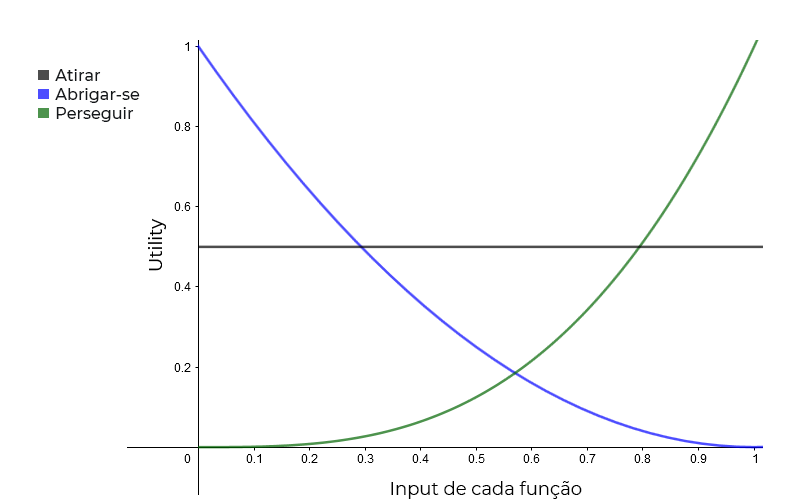
\includegraphics[width=34em]{imagens/utilityFunctions.png}
	\caption{Gráfico das funções utility}
\end{figure}

 
 Sobrepondo as três funções pode-se ter uma melhor noção de qual comportamento irá se sobressair em cada situação para cada valor do parâmetro. Entretanto, vale lembrar que os valores de vida e distância são independentes e portanto as funções não necessariamente estarão no mesmo ponto do eixo X ao mesmo tempo.
 A tabela abaixo demonstra três situações em que, para cada conjunto de parâmetros tem-se uma ação que é decidida usando a maior utility. O asterisco indica a função cuja pontuação foi maior e será, portanto, a ação executada.
 
 
\begin{table}[H]
\centering
\begin{tabular}{l l l l l}
vida & distância & Atirar & Abrigar-se & Perseguir \\
\hline		
0 & 0 & 0.5* & 0 & 0 \\
0.2 & 0 & 0.5 & 0.64* & 0 \\
0.2 & 0.5 & 0.5 & 0.64* & 0.125 \\
0.2 & 0.9 & 0.5 & 0.64 & 0.729* \\
0.3 & 0 & 0.5* & 0.49 & 0 \\

\end{tabular}
\caption{Tabela de valores exemplo para as funções de pontuação}
\end{table}

Por fim, o código de implementação é composto de três classes: Action, Consideration e ConsiderationTree. Um game object com IA recebe um componente com a árvore de considerações (\texttt{ComponentTree}). A árvore de considerações contem as possíveis ações que esse agente pode tomar. Cada consideração implementa um método \texttt{evaluate()} que recebe como parâmetro o contexto e dele extrai os valores de que precisa para realizar seus cálculos e retornar a \textit{utility}. A classe Action contém o nome daquela \textit{utility} para que o objeto possa se guiar e executar a ação associada. Ela contém também o alvo daquela ação, caso haja algum. Esse fluxo é demonstrado no diagrama de classes dado a seguir.

\begin{figure}[H]
	\centering
	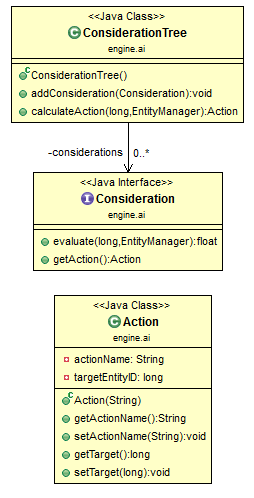
\includegraphics[width=13em]{imagens/considerationTree.png}
	\caption{Diagrama da Árvore de considerações para as funções de pontuação}
\end{figure}

%//TODO: good example https://alastaira.wordpress.com/2013/01/25/at-a-glance-functions-for-modelling-utility-based-game-ai/
%//https://www.gamasutra.com/blogs/JakobRasmussen/20160427/271188/Are_Behavior_Trees_a_Thing_of_the_Past.php

%\section{Finite State Machine}
%\section{Árvore de decisões}

\section{Pathfinding}
Existem muitos algoritmos de \textit{pathfinding} como, por exemplo, A*, Dijkstra's, LPA* entre outros . Alguns se adéquam muito bem para sistemas estáticos onde tem-se total conhecimento e controle do ambiente, enquanto outros são melhor adaptados para ambientes imprevisíveis e sob constante mudança.

Além dos vários algoritmos disponíveis e suas respectivas variações existem também diversas formas de representar o espaço de busca. Os algoritmos de \textit{pathfinding} trabalham em cima do conceito de grafos. Portanto, independentemente do jogo ser em 3D ou 2D, no final deverá haver uma representação desse mundo na forma de um grafo. Para um jogo 2D baseado em grids isso é facilmente alcançável aproveitando cada célula desse grid e transformando-a em um nodo do grafo. Para cada dois nodos adjacentes onde ambos são transponíveis há uma aresta que os liga. Se o mundo é construído sem utilizar diretamente o conceito de grid ainda é possível representá-lo em um grid com células de tamanho x e, caso uma célula intersecte a \textit{bounding box} de um objeto
ela torna-se intransponível.

Existe ainda a possibilidade de utilizar uma \textit{octree} onde cada célula desse grid possui tamanho potência de um valor estático, ao invés de um tamanho único e estático. Há ainda conceitos que usam polígonos convexos para gerar uma malha que particiona o mapa em pedaços transponíveis. De maneira geral, existem diversas técnicas e cada projeto deve optar por aquela que melhor lhe servir.

No sistema implementado na engine narval o processo de \textit{pathfinding} em ambiente 2D consiste em primeiro mapear a seção visível do mapa e mais um offset para uma matriz. Essa seção é geralmente o retângulo que constitui a visão do personagem. Para cada entidade que intersecta essa seção será feito um mapeamento da sua caixa de colisão para a matriz. Cada posição da matriz representa um retângulo de tamanho arbitrário e fixo. Note que, a não ser que todas as entidades do jogo possuam módulo zero com o tamanho do retângulo da matriz haverá um erro a se considerar. Por exemplo, se uma entidade com retângulo de 32x32 vai ser inserida em uma matriz cuja célula é um retângulo de 10x10, na hora do mapeamento essa entidade vai ocupar 4x4 células na matriz, tendo assim, para o algoritmo de pathfinding, um tamanho de 40x40. Isso resulta em um erro de 8 pixels para o tamanho real da entidade. Esse exemplo é demonstrado na figura a seguir, onde a parte vermelha representa a base box e a parte azul o desperdício. Ambas as duas partes representam o retângulo de fato contido na matriz.

\begin{figure}[H]
	\centering
	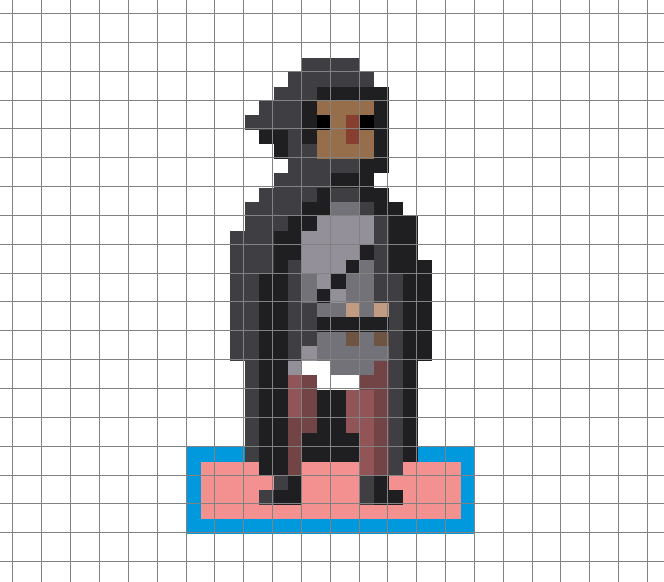
\includegraphics[width=22em]{imagens/pixelWaste.png}
	\caption{Desperdício gerado ao mapear uma base box de 32x32 pixels numa matriz de retângulos 10x10 pixels.}
\end{figure}


Uma vez realizado o mapeamento tem-se uma matriz boolena representando quais pontos são transponíveis. A partir disto basta implementar um algoritmo de busca como, por exemplo, o A* para percorrer o grafo representado pela matriz e encontrar um caminho do ponto A para um ponto B. É importante levar em consideração que os objeto podem ocupar mais de um nodo devido ao seu tamanho e isso possui implicação direta na implementação do algoritmo de busca.

\begin{figure}[H]
	\centering
	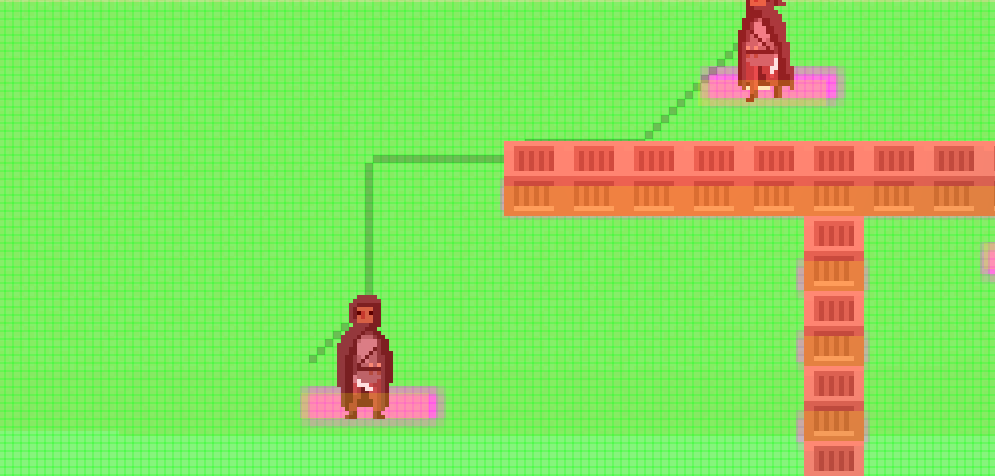
\includegraphics[width=30em]{imagens/pathPlanningWithGrid.png}
	\caption{Matriz booleana representada visualmente com os retângulos verdes sendo os transponíveis e os rosas intransponíveis. }
\end{figure}

\subsection{A*}
Para uma implementação utilizando A* é necessário considerar o ponto de início não como um único ponto, mas como um conjunto de pontos que representam a base box da entidade. Essa aproximação permite que uma entidade cuja base box ocupa mais de um nodo possa se locomover pelo grid.

O algoritmo de busca A* funciona determinando, a cada iteração, qual caminho estender. Isso é feito através da equação $f(n) = g(n) + h(n)$, onde $n$ é o próximo nodo no caminho, $g(n)$ o custo do nodo inicial até $n$ e $h(s)$ uma função heurística que estima o custo mais baixo do caminho de $n$ até o nodo objetivo.

A heurística utilizada considera a possibilidade de 8 direções no grid, atribuindo um maior custo para as diagonais. Como a heurística é apenas uma aproximação, define-se uma constante $\sqrt{2}$ para multiplicar a distância diagonal. Dessa forma, tem-se uma estimativa razoável sem o custo alto de realizar o cálculo completo da distância euclidiana $\sqrt{x^2 + y^2}$. Dessa forma, a função heurística $h(n)$ fica como se segue.

\begin{lstlisting}[caption= Heurística utilizada no A*]
    float a = Math.abs(start.pos.x - end.pos.x);
    float b = Math.abs(start.pos.y - end.pos.y);
    
    float min = Math.min(a,b);
    float max = Math.max(a,b);
    
    return ((M_SQRT2-1.0f)*min + max);
\end{lstlisting}


O código completo do algoritmo A* implementado pela engine é dado no apêndice~\ref{apend:alg:a*}. O resultado obtido é também demonstrado na imagem a seguir.

\begin{figure}[H]
	\centering
	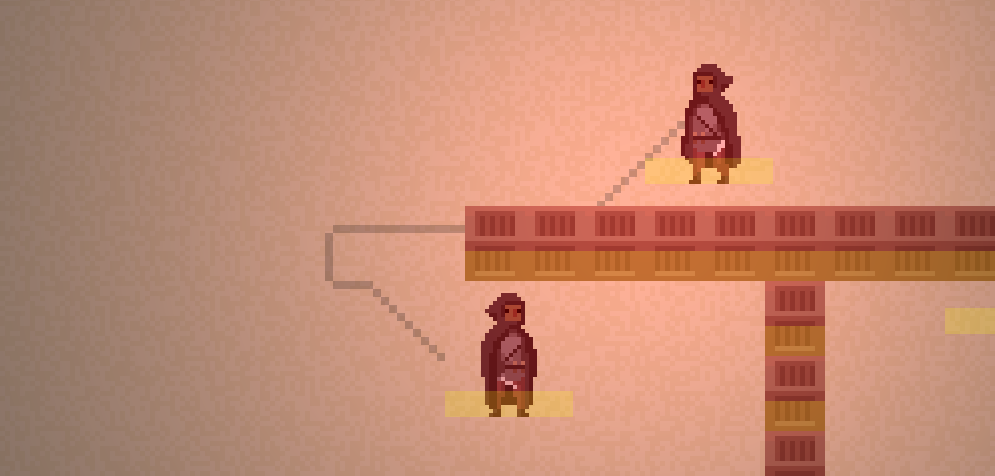
\includegraphics[width=30em]{imagens/pathPlanning.png}
	\caption{Resultado final obtido com o A* }
\end{figure}

\iffalse
//TODO: https://gamedev.stackexchange.com/questions/28041/path-finding-algorithms

//TODO: links dos comentarios são interessantes

//TODO: http://theory.stanford.edu/~amitp/GameProgramming/Heuristics.html

//TODO: https://www.growingwiththeweb.com/2012/06/a-pathfinding-algorithm.html
\fi

\chapter{Procedural Content Generation}
Procedural Content Generation (PCG) é o termo cunhado para descrever processos de geração de dados aleatórios ou pseudo-aleatórios em jogos. Esses dados são utilizados para criar regras que definem desde terrenos até modelos 3D de maneira algorítmica ao invés de manual.

\section{Random noise}
O conceito mais básico na construção de elementos baseados em PCG envolve a utilização de ruídos como fonte de dados pseudo-aleatória. Existem diversos algoritmos para obtenção de ruído pseudo-aleatório como, por exemplo, perlin noise, simplex noise e gradient noise. Há ainda técnicas que se utilizam de maneiras não determinísticas e implementam outras fontes de dados.

\subsection{Perlin noise}
Perlin noise é um tipo de ruído gradiente concebido por \citeonline{perlin1985image} e depois melhorado por ele mesmo em 2002 \cite{Perlin:2002:IN:566654.566636}. Esse algoritmo é comumente usado na indústria para geração de ruídos que são utilizados para criar texturas de água, fogo, terrenos, nuvens e muitos outros. O ruído pode ser representado em uma, duas, três ou até quatro dimensões.

O algoritmo recebe como entrada um ponto de $n$ coordenadas. Esse ponto deve ser unitário, ou seja, para cada coordenada faz-se $ mod~1$. Uma vez com as coordenadas unitárias em mãos elas são representadas em uma linha, quadrado ou cubo dependendo das dimensões do vetor. Por exemplo, para um vetor de duas dimensões com os valores $(0.75, 0.25)$ tem-se o seguinte ponto no plano:

\begin{figure}[H]
	\centering
	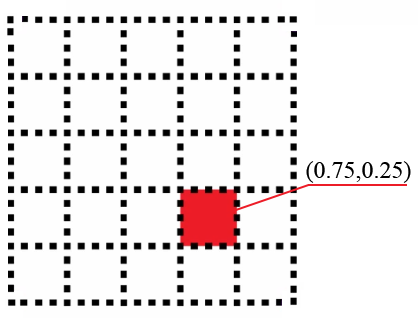
\includegraphics[width=15em]{imagens/perlinPoint.png}
	\caption{Ponto $(0.75, 0.25)$ no plano. Adaptado de: \cite{Fataho}}
\end{figure}

Para cada um dos 4 pontos unitários que definem a borda do plano (8 para o cubo em 3D), são gerados vetores gradiente de maneira pseudo aleatória. Com esse vetor gradiente definido ele é fixo para a função que se está trabalhando.

\begin{figure}[H]
	\centering
	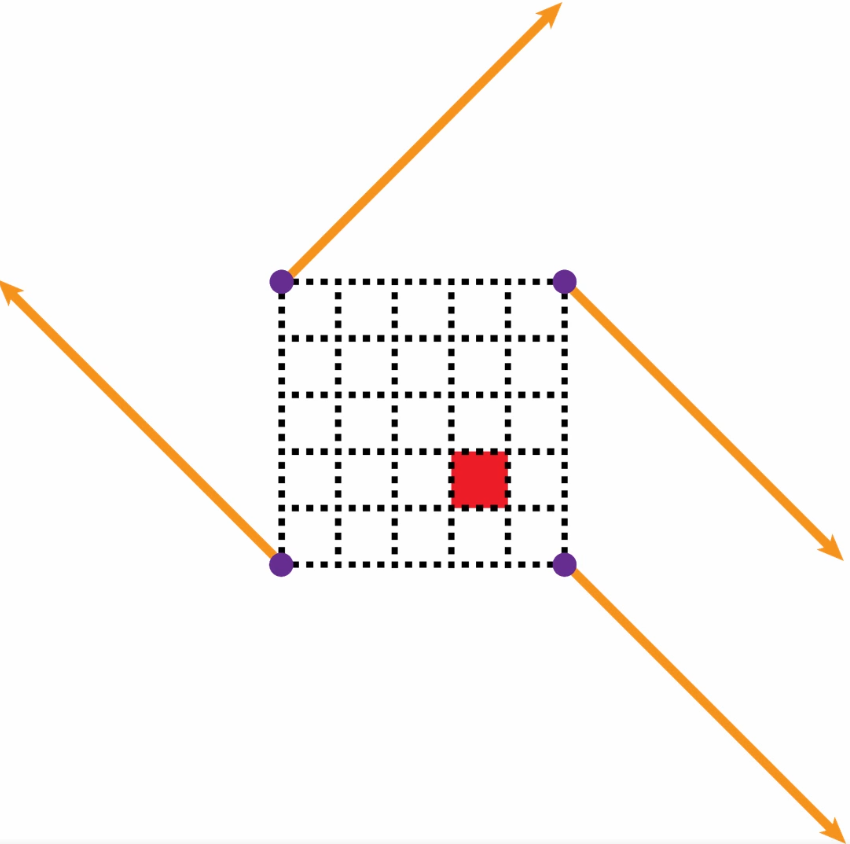
\includegraphics[width=15em]{imagens/perlinGradients.png}
	\caption{Vetores gradiente definidos em amarelo no plano. Adaptado de: \cite{Fataho}}
\end{figure}

Em posse do ponto e dos vetores gradientes é necessário agora calcular o vetor distância desse ponto até os quatro pontos na borda do plano.

\begin{figure}[H]
	\centering
	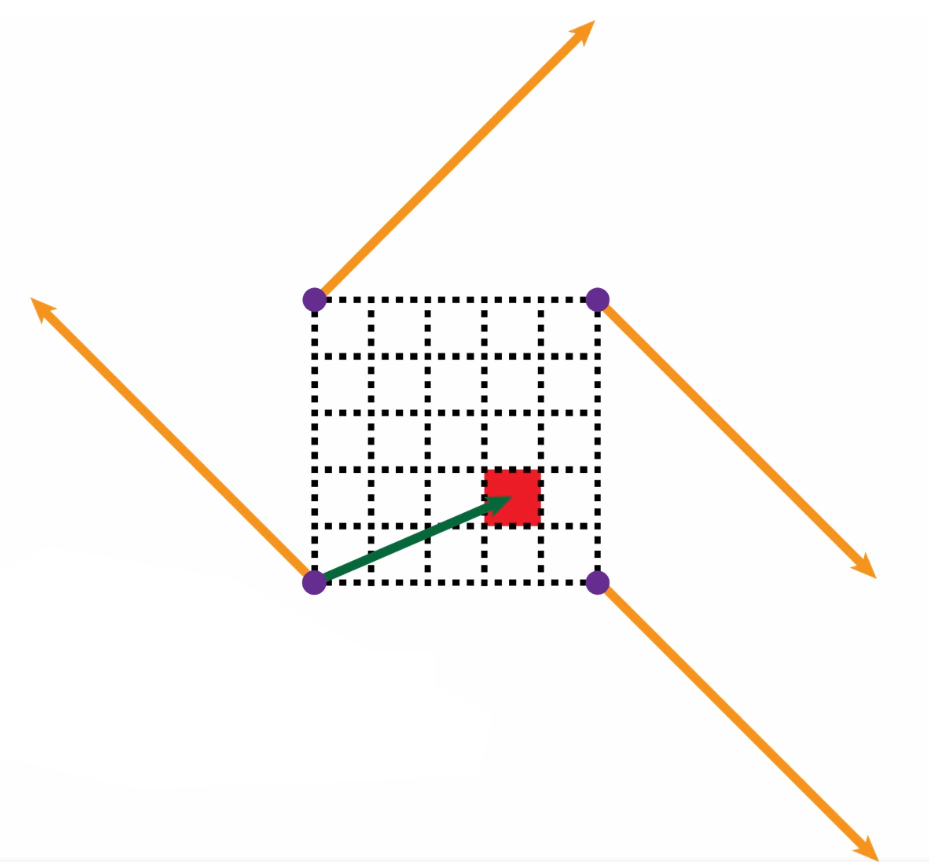
\includegraphics[width=15em]{imagens/perlinGradientsAndOneDistance.png}
	\caption{Vetor distância do ponto $(0,0)$na borda até o ponto $(0.75,0.25)$ em vermelho. Adaptado de: \cite{Fataho}}
\end{figure}

Uma vez com o vetor distância, vetor gradiente e o ponto dado como parâmetro da função realiza-se o produto escalar entre ambos os vetores para obter o valor $influência$.

$\vec{D} = \vec{G}(-1,1) ~\cdotp ~ \vec{D}(0.75, 0.25)$

$~~~~ = -1 * 0.75 + 1 *0.25$

$~~~~ = -0.75 + 0.25$

$~~~~ = -0.5$

Esse processo é realizado para os quatro pares de vetor gradiente e vetor distância. Em sentido anti-horário, começando do ponto inferior esquerdo, os valores $influência$ são $-0.5$, $-0.5$, $0.5$ e $0$.
\begin{figure}[H]
	\centering
	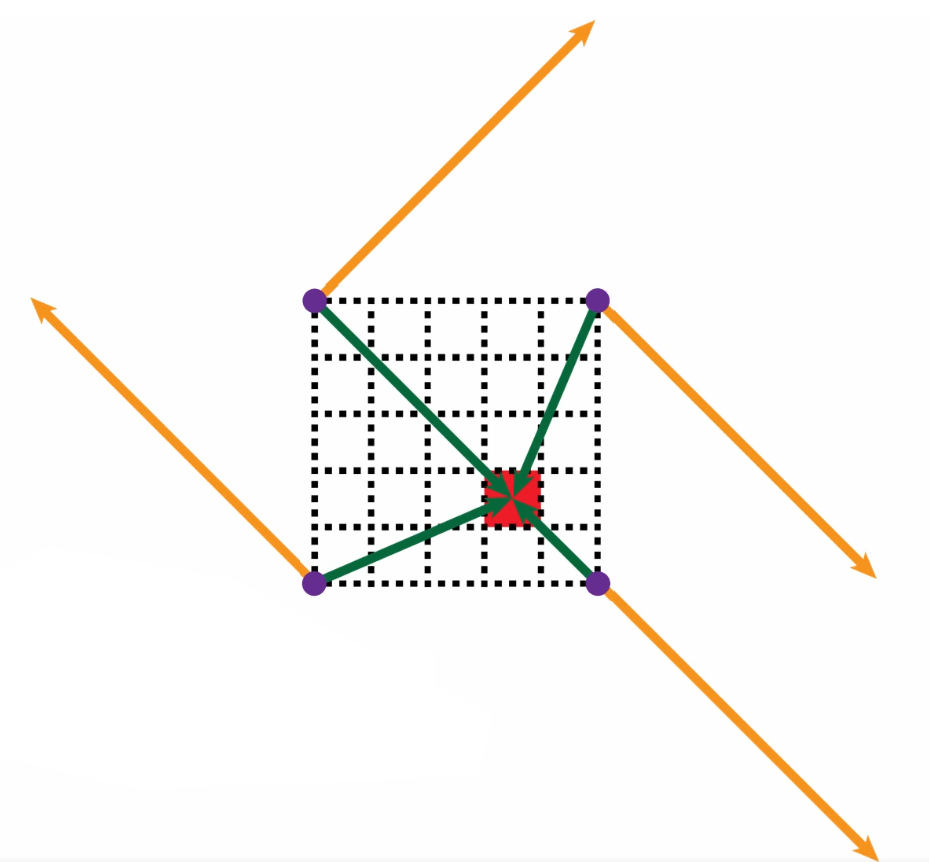
\includegraphics[width=15em]{imagens/perlinGradientsAndDistances.png}
	\caption{Vetores distância do ponto $(0,0)$ em verde e vetores gradiente em amarelo. Adaptado de: \cite{Fataho}}
\end{figure}

O último passo consiste em interpolar linearmente os 4 valores $influência$ \texttt{b1}, \texttt{b2}, \texttt{b3} e \texttt{b4} como demonstrado no algoritmo a seguir. O resultado final retornado pelo algoritmo do perlin noise será dado pela variável \texttt{result}.

\begin{lstlisting}[caption=Interpolação dos valores $influência$]
int b1, b2, b3, b4;
int x, y; 

int x1 = linearInterpolation(b1,b2,x);
int x2 = linearInterpolation(b3,b4,y);

int result = linearInterpolation(x1,x2,y);

float linearInterpolation(float a, float b, float t){
	return (1f - t) * a + t * b;
}
\end{lstlisting}
 

\section{Geração de terrenos}
A geração de terreno utilizada na engine consiste, num primeiro passo, em preencher um conjunto de matrizes com valores gerados por vários algoritmos de ruído na função \texttt{generateAndShapeNoise}, sendo o principal deles Perlin Noise. Cada um desses valores é então extraído da matriz e atribuído um significado baseado numa regra determinada pela função \texttt{generateTerrain}. Os ruídos são gerados utilizando a implementação \texttt{FastNoise} \cite{FastNoise} incorporado na engine, onde o valor retornado pelas funções de ruído geralmente está no intervalo [-1,1]. 

A textura gerada para lapidar o terreno é chamada de \textit{height map} e serve para indicar alturas no mapa. Com essa textura em mãos cada valor recebe um significado em termos de altura do terreno.

Ruídos podem ser gerados em qualquer frequência, que basicamente resultam no efeito de zoom da textura final. Esse efeito é consequência da fórmula do comprimento de onda $\lambda = \frac{velocidade}{frequência}$ onde, dobrando a frequência, implica em diminuir o comprimento de onda pela metade do seu tamanho.

\begin{figure}[H]
	\centering
	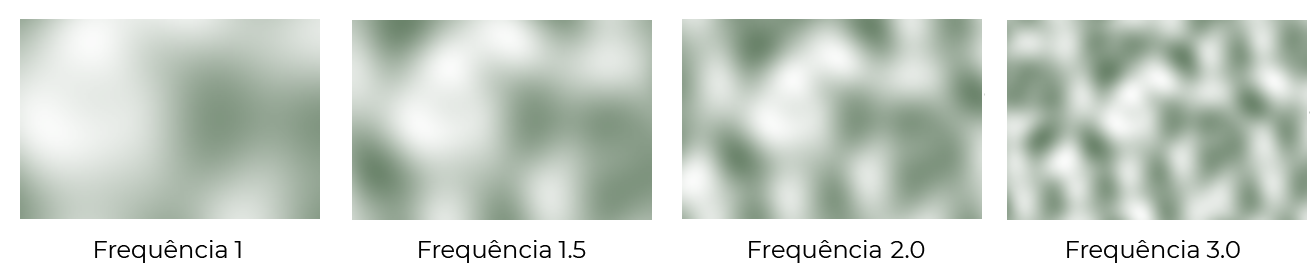
\includegraphics[width=34em]{imagens/perlinFrequencies.png}
	\caption{Resultado da alteração na frequência. Adaptado de: \cite{NoiseRedBlob}}
\end{figure}


Outro atributo importante no processo de modelagem do ruído são os \textit{octaves}. Eles servem para lapidar o ruído e adicionar mais detalhes na textura. Eles funcionam somando-se os ruídos gerados, mas cada um tendo uma frequência e peso diferente diferentes. Isso é demonstrado no código a seguir onde soma-se um perlin noise de frequência $0.0005$ com peso $1$ e outro de frequência $0.005$ com peso $0.1$, resultando em dois octaves.

\begin{lstlisting}[caption=Implementação do ruído que usa o perlin noise com dois octaves]
public float noise(FastNoise fastNoise, float x, float y) {
		float noise = 0;
		
		fastNoise.SetFrequency(0.0005f);	
		noise +=  fastNoise.GetPerlin(x, y);

		fastNoise.SetFrequency(0.005f);
		noise += .1 * fastNoise.GetPerlin(x, y);
		
		return noise;
	}
\end{lstlisting}   

Até então o ruído possui um aspecto fractal, com várias colinas e montanhas, mas nenhuma área de terreno plano. Para isso é necessário aplicar uma exponenciação ao ruído, achatando-o através da redução de valor. Não só é necessário um fator de exponenciação, mas também uma fórmula para gerar ruídos no formato de continentes e ilhas, onde quanto mais próximo da borda maior a probabilidade desse valor ser formatado como água. Essa fórmula consiste em primeiro calcular a distância de Manhattan $d$ do valor (x,y) atual até o centro do mapa e multiplicar por 2.

$d = 2*max(abs(x - center_x), abs(y - center_y))$

A segunda etapa consiste em calcular a fórmula dada em seguida \cite{NoiseRedBlob} onde $a$ é uma constante que puxa os todos os valores para cima, $b$ puxa as bordas do mapa para baixo e $c$ controla o quão rápido essa queda é.

$ noise = noise + a - b*d^c$

Dessa forma, o código completo da implementação que calcula e modela o ruído para uso é dado a seguir.

\begin{lstlisting}[caption=Implementação que gera e molda o ruído]
public void generateAndShapeNoise() {
		float d;
		float a = 0.15f;
		float b = 0.9f;
		float c = 2f;
		
		int coordX = ((this.x*chunkWidth)/NOISE_DIVISOR)  ;
		int coordY = ((this.y*chunkHeight)/NOISE_DIVISOR)  ;

		int constX = coordX;
		int constY = coordY;
		
		for(int y=0; y<textureHeight; y++) {
			for(int x=0; x<textureWidth;x++) {
				coordX = constX + x;
				coordY = constY + y;
				
				d = 2*Math.max(Math.abs((float)coordX/mapWidth - (float)(mapWidth/2)/mapWidth), Math.abs((float)coordY/mapHeight - (float)(mapHeight/2)/mapHeight));
				
				perlinNoise[x][y] = noise(fastNoise,coordX/3f,coordY);
				whiteNoise[x][y] = fastNoise.GetWhiteNoise(coordX, coordY); 
				fractalNoise[x][y] = fastNoise.GetPerlinFractal(coordX/4, coordY); 
				
				perlinNoise[x][y] = perlinNoise[x][y] + a - b*(float)Math.pow(d, c);
			}
		}
	}
\end{lstlisting}  

A última etapa é atribuir um significado para cada um desses valores gerados. O código completo da implementação que atribui um significado a esses valores é dada a seguir. Em suma, valores abaixo de $-0.255$  viram água, valores abaixo de $-0.1$ viram areia e valores acima disso viram terra.

\begin{lstlisting}[caption=Implementação que gera a textura final do terreno]
public void generateTerrain() {

	for(int y=0; y<textureHeight; y++) {
		for(int x=0; x<textureWidth;x++) {
			
			if(perlinNoise[x][y]>-.1 ) { 		//terra
				mapRGB[x][y] = Color.GRASS_GROUND;
				if(fractalNoise[x][y]>0.2)
					mapRGB[x][y] = Color.GRASS_GROUND_LIGHTER;
			}
			
			if(perlinNoise[x][y]<=-.1) {	//areia
				mapRGB[x][y] =  (255<<24) | (244<<16) | (234<<8) | (187);
				if(whiteNoise[x][y]>0)
					mapRGB[x][y] =  (255<<24) | (234<<16) | (224<<8) | (167);
			}
			
			if(perlinNoise[x][y]<=-.255)  //preenche tudo com agua
				mapRGB[x][y] = 	Color.TURKISH; //turquesa
		}
	}
}
\end{lstlisting}    

Os resultados obtidos possuem terrenos de formato de similar aos exemplificados na figura a seguir.

\begin{figure}[H]
	\centering
	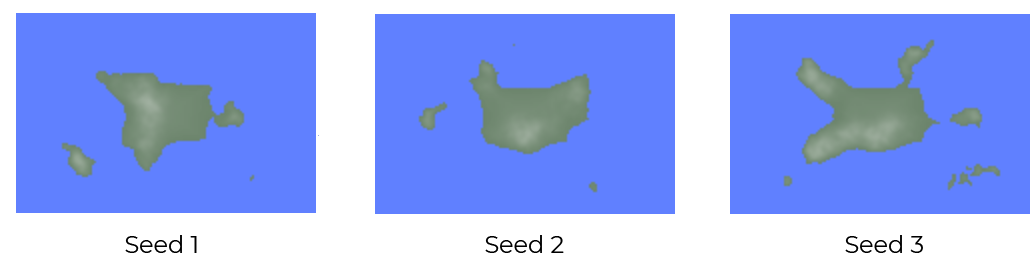
\includegraphics[width=34em]{imagens/generatedTerrains.png}
	\caption{Resultado final dos terrenos após modelagem do ruído e atribuição de significado. Adaptado de: \cite{NoiseRedBlob}}
\end{figure}

%//TODO: good source: https://thebookofshaders.com/12/ http://pcgbook.com/

\chapter{Diagramas e panorama geral}
\label{cap:panoramaGeral}

Os diagramas dados a seguir descrevem toda a estrutura que compõe a fundação da engine Narval. Juntamente com o código ao longo deste trabalho os diagramas são a realização dos módulos abordados e descritos na introdução do capítulo \ref{cap:gameEngine}.

Todas as classes até então desenvolvidas e abordadas se organizam nos pacotes descritos pela figura \ref{fig:arquitetura} e são dadas formalmente a seguir. Cada pacote agrupa classes relacionadas à um tema, área ou módulo da engine.

\section{Pacote de IA}

O pacote \texttt{engine.ai} contém todas as classes relacionadas à implementação de inteligência artificial. Essas classes implementam o A* e o conceito de utility utilizado para tomada de decisões do agente.

\begin{figure}[H]
	\centering
	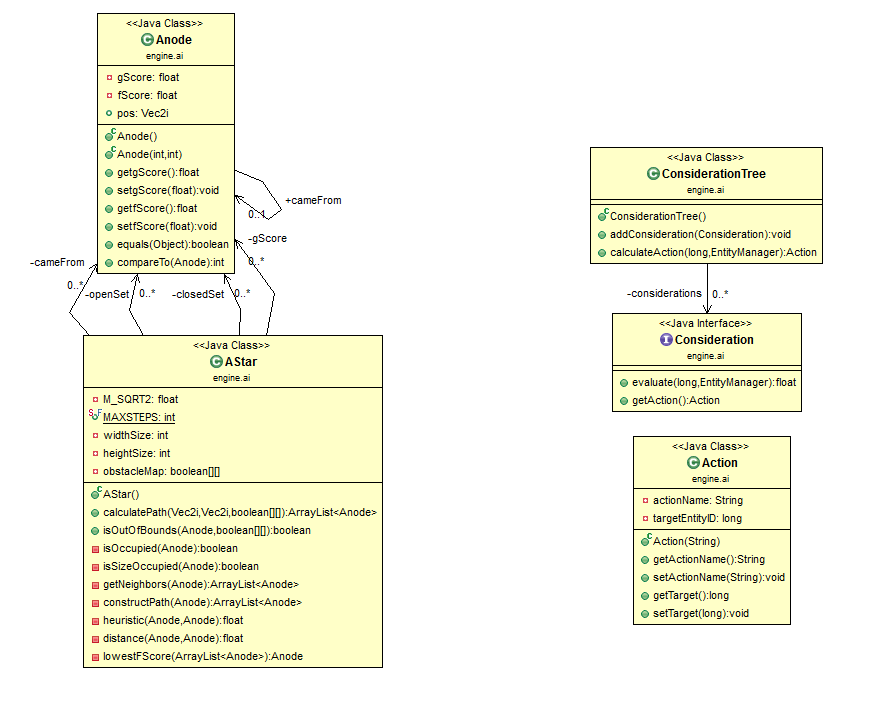
\includegraphics[width=30em]{imagens/engine.ai.png}
	\caption{Classes do pacote engine.ai}
\end{figure}

\section{Pacote de Aúdio}

O pacote \texttt{engine.audio} contém todas as classes relacionadas à implementação de áudio. Essas classes implementam a leitura e configuração do arquivo de áudio via OpenAL.

\begin{figure}[H]
	\centering
	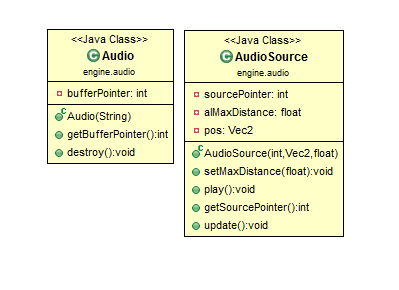
\includegraphics[width=22em]{imagens/engine.audio.png}
	\caption{Classes do pacote engine.audio}
\end{figure}

\section{Pacote da Engine}

O pacote \texttt{engine.engine} contém todas as classes relacionadas à implementação do núcleo da game engine. Essas classes implementam a thread onde será rodada a primeira chamada ao método update e render, bem como a engine de física e também a janela OpenGL onde deverá ser feita a renderização. É nesse pacote também que serão carregadas e definidas todas as configurações da engine.

\begin{figure}[H]
	\centering
	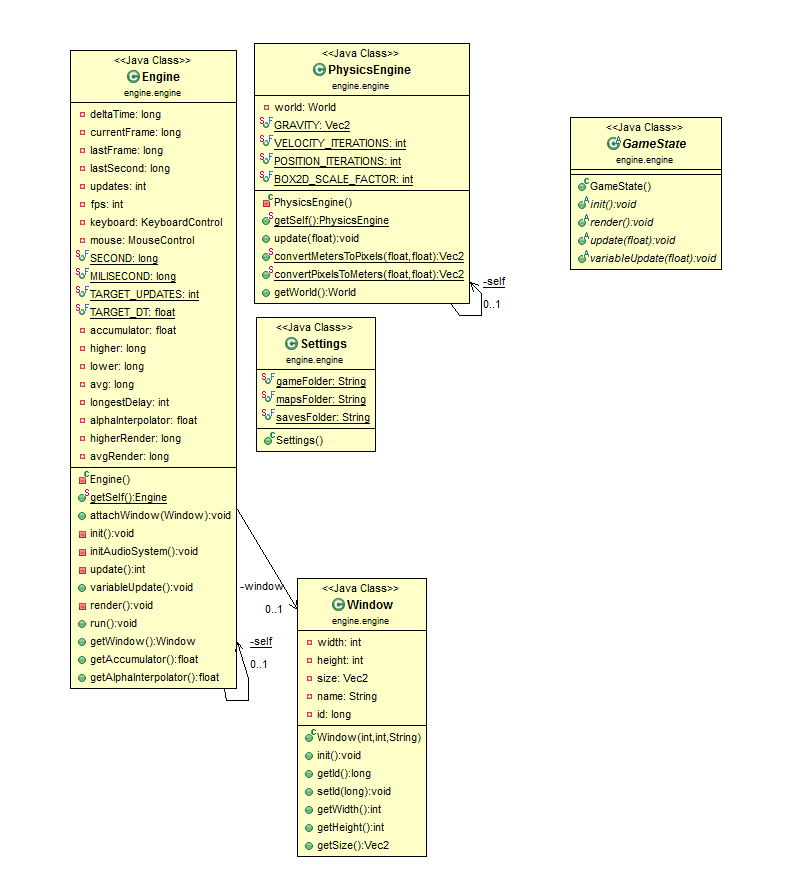
\includegraphics[width=30em]{imagens/engine.engine.png}
	\caption{Classes do pacote engine.engine}
\end{figure}

\section{Pacote de componentes de entidades}

O pacote \texttt{engine.entity.component} contém todas as classes relacionadas à implementação dos componentes das entidades. Muito embora cada jogo deverá ter seus próprios componentes, esse pacote implementa os mais comuns que estarão presentes em, senão todos os jogos, a maioria significativa deles.

\begin{figure}[H]
	\centering
	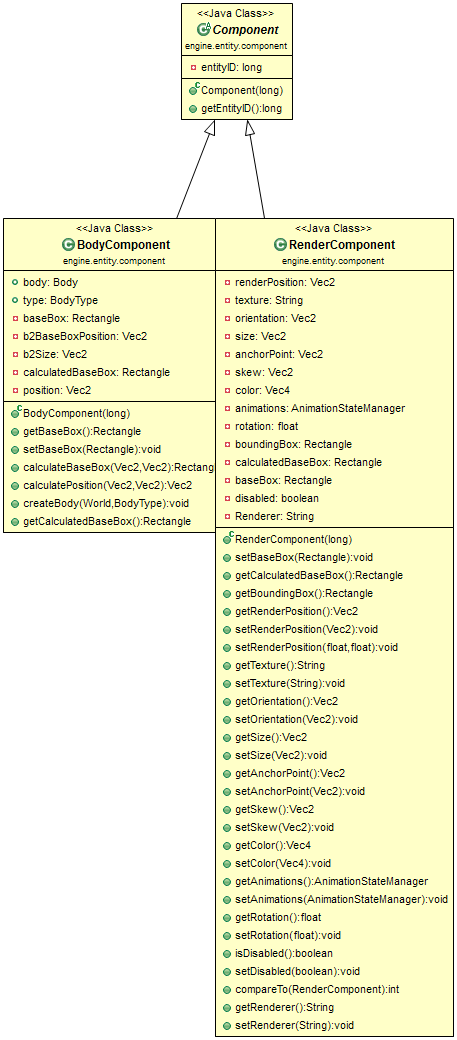
\includegraphics[width=22em]{imagens/engine.entity.component.png}
	\caption{Classes do pacote engine.entity.component}
\end{figure}

\section{Pacote de entidades}

O pacote \texttt{engine.entitiy} contém todas as classes relacionadas à implementação das entidades e os sistemas que as gerenciam. Também conta com a implementação de algumas especializações comuns em jogos.

\begin{figure}[H]
	\centering
	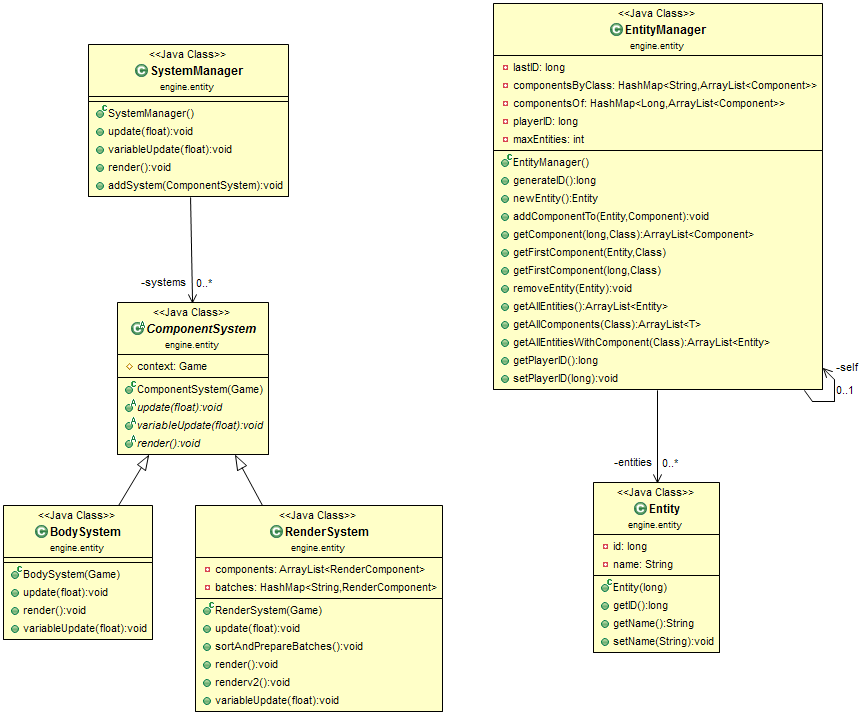
\includegraphics[width=22em]{imagens/engine.entity.png}
	\caption{Classes do pacote engine.entity}
\end{figure}

\section{Pacote gráfico}

O pacote \texttt{engine.graphic} contém todas as classes relacionadas à implementação dos componentes gráficos como animações, textura e os shaders utilizados pelo OpenGL.

\begin{figure}[H]
	\centering
	\includegraphics[width=22em]{imagens/engine.graphic.png}
	\caption{Classes do pacote engine.graphic}
\end{figure}


\section{Pacote de input}

O pacote \texttt{engine.input} contém todas as classes relacionadas ao tratamento de input.

\begin{figure}[H]
	\centering
	\includegraphics[width=22em]{imagens/engine.input.png}
	\caption{Classes do pacote engine.input}
\end{figure}


\section{Pacote lógico}

O pacote \texttt{engine.logic} contém classes relacionadas ao aspecto lógico geral do sistema. Ele contém o sistema de chunks, timer, camera e o sistema de gerenciamento de animações.

\begin{figure}[H]
	\centering
	\includegraphics[width=24em]{imagens/engine.logic.png}
	\caption{Classes do pacote engine.logic}
\end{figure}

\section{Pacote de ruído}

O pacote \texttt{engine.noise} contém a classe responsável por gerar o ruído utilizado na construção dos mapas. Sendo ela uma implementação de licença MIT feita por Auburns.

\begin{figure}[H]
	\centering
	\includegraphics[width=24em]{imagens/engine.noise.png}
	\caption{Classes do pacote engine.noise}
\end{figure}
//TODO : referencias às figuras e recortar a imagem


\section{Pacote de renderizadores}

O pacote \texttt{engine.renderer} contém as classes responsáveis pelos tipos de renderização.

\begin{figure}[H]
	\centering
	\includegraphics[width=24em]{imagens/engine.renderer.png}
	\caption{Classes do pacote engine.renderer}
\end{figure}

\section{Pacote de utilidades}

O pacote \texttt{engine.utilities} contém uma série de classes consideradas utilitárias como por exemplo, criação e conversão de buffers, leitura de arquivos, conversão de cores, funções matemáticas e muitas outras.

\begin{figure}[H]
	\centering
	\includegraphics[width=24em]{imagens/engine.utilities.png}
	\caption{Classes do pacote engine.utilities}
\end{figure}

\section{Estrutura dos arquivos}
A estrutura geral de arquivos e pacotes do projeto da Engine Narval é dada a seguir. Cada arquivo representa uma classe Java e cada pasta é denotada por uma barra e considerada como um pacote do projeto.

\begin{lstlisting}[caption=Árvore de arquivos do projeto]
Engine
    /ai
        Action
        AStar
        Anode
        Consideration
    /audio
        Audio
        AudioSource
    /controllers
        Controller
        PlayerController
    /engine
        Engine
        GameState
        PhysicsEngine
        Settings
        Window
    /entity
        /component
            Component
            PositionComponent
            RenderCOmponent
        SystemManager
        PositionSystem
        RenderSystem
    /geometry
        Rectangle
        Segment
    /graphic
        Shader
        Animation
        Texture
    /input
        Control
        JoystickControl
        KeyboardControl
        MouseControl
    /logic
        Camera
        Chunk
        ChunkMap
        ReadingChunk
        SavingChunk
        Timer
    /noise
        FastNoise
    /renderer
        AnimationsManager
        Renderer
        TextureRenderer
        BatchTextureRenderer
    /ui
        Font
        Glyph
    /utilities
        ResourceManager
        ArraysExt
        BufferUtilities
        Color
        GLFWUtil
        MathExt
        QuadTree
\end{lstlisting}        



\iffalse
\chapter{Criação de um protótipo}

\label{sec:desenv}
\section{Mecânicas}
\subsection{Sistema de caça ativa}
\begin{figure}[H]
	\centering
	\includegraphics[width=4in]{imagens/mecanica_caca.png}
	\caption{Jogador caçando um coelho com arco e flecha}
\end{figure}
O sistema de caça é dado pelo seguinte fluxo de ações:
\begin{enumerate}  
\item Jogador avista animal em ambiente selvagem 
\item Ao se aproximar o animal pode perceber sua presença. Caso seja notado, a presa irá executar uma animação indicando que está desconfiado.
\item Se o jogador continuar avançando o animal irá tentar fugir 
\item Senão o jogador executa um ataque quando estiver ao alcance 
\end{enumerate}


\subsection{Sistema de armadilhas}
\begin{figure}[H]
	\centering
	\includegraphics[width=4in]{imagens/mecanica_armadilha.png}
	\caption{Jogador pronto para atacar alvo que ficou preso na armadilha de chão}
\end{figure}
O sistema de armadilhas é dado pelo seguinte fluxo de ações:
\begin{enumerate}  
\item Jogador aciona armadilha no local desejado
\item Qualquer animal ou inimigo pode acionar a armadilha e acionar o seu efeito
\end{enumerate}

\subsection{Sistema de Combate}
O sistema de combate é delimitado pela arma escolhida. Cada arma implica em um estilo
de combate totalmente diferente e só pode ser utilizada ao aprender esse estilo com um
mestre. Os mestres podem ser encontrados aleatoriamente pelo mapa em grandes cidades de 
cada reino.

\subsection{Sistema de apadrinhamento}
Ao atingir um nível significante de reputação o jogador pode tentar ganhar um apadrinhamento de um rei ou lorde. Ganhando assim uma quantia semanal e benefícios como alimento e teto para poder compor suas músicas.

\subsection{Cantar músicas}
\begin{figure}[H]
	\centering
	\includegraphics[width=4in]{imagens/mecanica_cantar.png}
	\caption{Jogador cantando em um vilarejo}
\end{figure}
\begin{figure}[H]
	\centering
	\includegraphics[width=4in]{imagens/mecanica_cantar2.png}
	\caption{Jogador sendo prestigiado após término da música}
\end{figure}
Cada vilarejo ou cidade tem um nível de interesse próprio em determinados instrumentos.
Quanto maior o interesse, maior serão as chances de receber uma boa quantia em ouro
pela apresentação.
As músicas podem ser tocadas em fogueiras que o próprio jogador pode criar em volta da cidade, ou em tavernas, festivais e praças.
\subsection{Compor músicas}
\begin{figure}[H]
	\centering
	\includegraphics[width=4in]{imagens/mecanica_compormusica.png}
	\caption{Esboço do menu para compor músicas}
\end{figure}
ASD.
\subsection{Contar histórias}
ASD.
\subsection{Compor histórias}
ASD.
\subsection{Atributos dos vilarejos e cidades}
Cada cidade e vilarejo possui os seguintes atributos:
\begin{description}  
\item [Lista de interesses instrumentais] Cada vilarejo tem uma preferência por um instrumento. Quanto maior o interesse, maior a recompensa dada ao tocar músicas com aquele instrumento.
\end{description}

\subsection{Atributos do jogador}
\begin{description}  
\item [Fome] Ao longo do tempo o jogador precisa se alimentar para manter-se vivo. A fome é dividida em três estágios: Sem fome, fome controlável e faminto. Cada um dos estágios é
apresentado ao jogador em forma de uma animação de andar diferente. Quanto mais faminto o personagem está mais lento e curvado ele irá andar, até que ela chegue em zero e culmine na morte do personagem.
\end{description}

\subsection{Domar animais}
Alguns animais podem ser domados através dos instrumentos. Basta cantar próximo a eles então eles serão domados.
\fi


% ------------------------------------------
% EXPERIMENTOS E RESULTADOS
\chapter{Experimentos e resultados}
\label{sec:experim}

\section{Demonstração}

A demonstração final construída utilizando a game engine evidência suas principais funcionalidades em um mini jogo de exploração com ambiente procedural 2D.

Nele pode-se caminhar através do cenário explorando o território gerado em tempo real e vislumbrar praias e florestas. Durante essa jornada pode-se notar o efeito de iluminação local, global e sua atenuação juntamente com o passar do dia.  Nota-se ainda o efeito de vento aplicado aos objetos que compõem a vegetação e entidades de AI simples que vagam pelo ambiente. A seguir são dadas algumas capturas de tela da demonstração. Cada captura de tela exemplifica uma das funcionalidades da engine discutidas no capítulo \ref{cap:gameEngine}.


\begin{figure}[H]
	\centering
	\includegraphics[width=24em]{imagens/ss1.png}
	\caption{Captura de tela 1}
\end{figure}

\begin{figure}[H]
	\centering
	\includegraphics[width=24em]{imagens/ss2.png}
	\caption{Captura de tela 2}
\end{figure}
\begin{figure}[H]
	\centering
	\includegraphics[width=24em]{imagens/ss3.png}
	\caption{Captura de tela 3}
\end{figure}
\begin{figure}[H]
	\centering
	\includegraphics[width=24em]{imagens/ss4.png}
	\caption{Captura de tela 4}
\end{figure}
\begin{figure}[H]
	\centering
	\includegraphics[width=24em]{imagens/ss5.png}
	\caption{Captura de tela 5}
\end{figure}


\iffalse
\section{Otimizações e testes de desempenho}

Perlin noise  vs GPU? ou noiseSize text mult

IMPLEMENTAR O BATCH RENDERING ANTES DE REALIZAR E DEMONSTRAR OS TESTES

Batch Rendering vs One draw call per object

Real time PCG x Loading chunk

Leitura assincrona vs sincroca

\fi

% ------------------------------------------
% CONCLUSÃO

\chapter{Conclusão}
\label{sec:conclus}
Com a primeira versão da game engine finalizada é necessário realizar algumas considerações finais. Um sistema dessa magnitude deve ser constantemente atualizado com novas tecnologias para manter-se relevante em um cenário competitivo como a indústria de jogos. A pesquisa permitiu produzir um extenso material em língua portuguesa acerca do tema, documentando e exemplificando cada etapa, desde a demonstração das amplas possibilidades para cada situação até sua implementação.

Embora distante de uma versão final, o projeto estando nessa etapa possui uma fundação sólida que lhe permite ser ampliado e melhorado para versões futuras. A engine não somente está com uma base bem construída, mas também está apta a ser utilizada na construção de jogos menos complexos.

Por ser um sistema de grande porte ele não somente embarca muitas funcionalidades, mas também muitas áreas do conhecimento. Por consequência direta disso muitas delas ainda devem sofrer ajustes ao longo do tempo para atingirem um patamar de alta qualidade. Isso só será obtido através de tempo e, muito possivelmente, pela atuação direta de profissionais qualificados da área.

Em suma, a construção de uma game engine é a junção do esforço de diversas áreas para criar um software capaz de trazer novos mundos e entretenimento ao grande público através da arte digital.

\section{Perspectivas de Trabalhos Futuros}

Para versões futuras da engine Narval espera-se uma portabilidade para novas APIs gráficas como DirectX e Vulkan. Também espera-se o desenvolvimento de um editor de níveis que permita uma interface mais abrangente e acessível ao usuário comum. Pretende-se elaborar e criar um suporte para renderização 3D, bem como a expansão e utilização de técnicas mais avançadas de renderização para efeitos sofisticados.

Muito embora essa versão esteja finalizada, espera-se um dia lançá-la no mercado sob a forma de um produto muito bem polido. Para isso tem-se ainda muitas etapas que devem ser superadas para atingir este objetivo final. Algumas delas envolvem não somente aspectos da renderização, mas também aspectos mais gerais como uma manipulação mais eficiente de arquivos, criação de ferramentas para scripting, resolução de pathfinding usando multithreading e muitos outros.



% ----------------------------------------------------------
% ELEMENTOS PÓS-TEXTUAIS


% ----------------------------------------------------------
\postextual

% ----------------------------------------------------------
% Referências bibliográficas
% ------------------------------------------
% REFERÊNCIAS MODELO DA FACOM
\bibliography{referencias}


% OS COMENTÁRIOS ABAIXO É CASO O TRABALHO TENHA ALGUM APÊNDICE
%% Apêndices TCC: só mantenha se for pertinente.
%% ----------------------------------------------------------

% ---
% Inicia os apêndices
% ---
\begin{apendicesenv}

% Imprime uma página indicando o início dos apêndices
%\partapendices

% ----------------------------------------------------------
\chapter{Implementação do Algoritmo A* Adaptado}
\label{apend:alg:a*}
% ----------------------------------------------------------
\begin{lstlisting}[caption=A* adaptado]
public class AStar {
	private ArrayList<Anode> openSet = new ArrayList<>();
	private ArrayList<Anode> closedSet = new ArrayList<>();
	private float M_SQRT2 = (float) Math.sqrt(2.0);
	public static final int MAXSTEPS = 900;
	private int widthSize = (128/8) +1, heightSize = (20/8)+1;
	private boolean obstacleMap[][];
	
	public ArrayList<Anode> calculatePath(Vec2i start, Vec2i end, boolean obstacleMap[][]){
		Anode startNode = new Anode();
		Anode endNode	= new Anode();
		Anode current;
		this.obstacleMap = obstacleMap;
		
		startNode.pos 	= start;
		endNode.pos 	= end;
		
		startNode.setgScore(0);
		startNode.setfScore( heuristic(startNode, endNode)  );
		
		openSet.add(startNode);
		
		int k=0;
		int index = 0;
		while(!openSet.isEmpty()) {
			if (k++ > MAXSTEPS) 
				return null;
			
			Collections.sort(openSet);
			
			current = openSet.get(0);
			
			if(current.pos.compareTo(endNode.pos) == 0) 
				return constructPath(current);
			
			openSet.remove(current);
			closedSet.add(current);
			
			for(Anode neighbor: getNeighbors(current)) {
				if(isSizeOccupied(neighbor))
					closedSet.add(neighbor);
				
				if(closedSet.contains(neighbor))
					continue; //ignore the neighbor which is already evaluated
				
				if(!openSet.contains(neighbor)) //discover new node
					openSet.add(neighbor);
						
				float gScore = current.getgScore() + distance(current,neighbor);
				if(gScore >= neighbor.getgScore())
					continue; // not a better path
				
				neighbor.cameFrom = current;
				neighbor.setgScore( gScore );
				neighbor.setfScore( neighbor.getgScore() + heuristic(neighbor, endNode) );
			}
		}
		
		return null;
	}
	
	public boolean isOutOfBounds(Anode node, boolean obstacleMap[][]) {
		if(node.pos.x>obstacleMap.length-1 || node.pos.y>obstacleMap[0].length-1 || node.pos.x<0 || node.pos.y<0)
			return true;
		return false;
	}
	
	private boolean isOccupied(Anode a) {
		return (!isOutOfBounds(a, obstacleMap) && obstacleMap[a.pos.x][a.pos.y]);
	}
	
	private boolean isSizeOccupied(Anode u) {
		Anode tempState = new Anode(u.pos.x , u.pos.y);
		
		for(int y=0; y<heightSize; y++) {
			for(int x=0; x<widthSize; x++) {
				tempState.pos.x = u.pos.x + x;
				tempState.pos.y = u.pos.y + y;
				
				if(isOccupied(tempState))
					return true;
			}
		}
		
		return false;
	}
	
	private ArrayList<Anode> getNeighbors(Anode current){
		ArrayList<Anode> neighbors = new ArrayList<>();
		Anode temp;
		
		temp = new Anode(current.pos.x + 1, current.pos.y);
		neighbors.add(temp);
		
		temp = new Anode(current.pos.x + 1, current.pos.y + 1);
		neighbors.add(temp);
		
		temp = new Anode(current.pos.x , current.pos.y + 1);
		neighbors.add(temp);
		
		temp = new Anode(current.pos.x - 1, current.pos.y + 1);
		neighbors.add(temp);
		
		temp = new Anode(current.pos.x - 1, current.pos.y);
		neighbors.add(temp);
		
		temp = new Anode(current.pos.x - 1, current.pos.y - 1);
		neighbors.add(temp);
		
		temp = new Anode(current.pos.x , current.pos.y - 1);
		neighbors.add(temp);
		
		temp = new Anode(current.pos.x + 1, current.pos.y - 1);
		neighbors.add(temp);
				
		return neighbors;
	}
	
	private ArrayList<Anode> constructPath(Anode current){
		Anode temp = current;
		ArrayList<Anode> path = new ArrayList<>();
		
		while(temp.cameFrom!=null) {
			path.add(temp.cameFrom);
			temp = temp.cameFrom;
		}
		
		return path;
	}
	
	private float heuristic(Anode start, Anode end) {
		float temp;
		float min = Math.abs(start.pos.x - end.pos.x);
		float max = Math.abs(start.pos.y - end.pos.y);
		
		if (min > max){
			temp = min;
			min = max;
			max = temp;
		}
		
		return ((M_SQRT2-1.0f)*min + max);
	}
	
	private float distance(Anode a, Anode b){
		float x = a.pos.x-b.pos.x;
		float y = a.pos.y-b.pos.y;
		return (float) Math.sqrt(x*x + y*y);
	}
	
	private Anode lowestFScore(ArrayList<Anode> list) {
		Anode current = list.get(0);
		
		for(Anode a: list) {
			if(current.getfScore()>a.getfScore())
				current = a;
		}
		
		return current;
	}
}

\end{lstlisting}

%\lipsum[50]

% ----------------------------------------------------------
%\chapter{Coisas que fiz e que achei interessante mas não tanto para entrar no corpo do texto}
% ----------------------------------------------------------
%\lipsum[55-57]

\end{apendicesenv}
% ---


% ----------------------------------------------------------
% Anexos %TCC: so mantenha se pertinente.
% ----------------------------------------------------------

% ---
% Inicia os anexos
% ---
%\begin{anexosenv}

% Imprime uma página indicando o início dos anexos
%\partanexos

% ---
%\chapter{Eu sempre quis aprender latim}
% ---
%\lipsum[30]

% ---
%\chapter{Coisas que eu não fiz mas que achei interessante o suficiente para colocar aqui}
% ---

%\lipsum[31]

% ---
%\chapter{Fusce facilisis lacinia dui}
% ---

%\lipsum[32]

%\end{anexosenv}

%---------------------------------------------------------------------
% INDICE REMISSIVO
%---------------------------------------------------------------------

\printindex



\end{document}